\part{De la numérisation à la numérisation de masse}

%====================CHAPITRE 1 keyword:histoire
\chapter{Historique de la numérisation}
Les projets de numérisation de masse ne sont pas soudainement apparus avec le tournant des années 2000, ils sont le fruit d'une multitude de développements technologiques et des transformations sociétales qui en découlent, initiés dès le 19\up{e} siècle. Ce premier chapitre vise à replacer ces projets au sein d'un contexte historique, entre l'émergence du web et la formation des premières bibliothèques numériques, sans oublier les débats politiques associés à ces projets culturels. 

Au même titre que les projets actuels combinent différents enjeux et acteurs, le développement de ces entreprises de numérisation sont au croisement des sciences de l'information et de l'informatique, et puisent leurs origines dans les deux domaines. Ce sont les progrès menés dans l'un et l'autre qui permettront la naissance des bibliothèques numériques dans les années 90, puis le passage à l'échelle des projets de numérisation. Nous verrons que l'idée des premières collections numériques existait bien avant, mais ces collections n'étaient pas identifiées en tant que tel\footnote{\cite[p. 8]{xie_discover_2016}}. 

Time Machine n'est pas le premier projet qui vise à mettre les données du passé à disposition du plus grand nombre, d'autres projets se sont construits autour d'objectifs similaires, avant même l'avènement du numérique.

 Afin de ne pas alourdir plus que nécessaire notre mémoire, nous avons choisi de présenter une sélection des personnalités et des projets qui nous ont semblé les plus emblématiques et les plus à même d'illustrer les différentes évolutions de ces précurseurs des initiatives de numérisation. 

%========PREMISSES DES PROJETS DE NUMERISATION
\section{1800-1990 : Prémisses des projets de numérisation}
Préalablement à l'émergence des bibliothèques numériques et aux projets de numérisation de masse, et bien que leurs origines soient quelque peu incertaines à retracer, des scientifiques et penseurs ont contribué par leurs idées et outils, à poser les jalons de ce que deviendront les grandes entreprises de numérisation. Au-delà de la naissance des éléments théoriques propres aux bibliothèques numériques, les développements du matériel informatique, de l'hypertexte, de l'internet et du web ont permis la naissance des infrastructures techniques nécessaires à la concrétisation de ces idées. Sans vouloir en dresser une liste exhaustive, il est intéressant de montrer que l'histoire de la numérisation à grande échelle est basée sur les mêmes fondements historiques qui ont vu la naissance du web que nous connaissons aujourd'hui. 
Une frise temporelle, reprenant les éléments propres à l'histoire de la numérisation et élargissant sur l'histoire du web est détaillée en annexe \ref{premisse}.

L'invention du microfilm, breveté par le français René Dagron en 1859, ouvre pour la première fois la perspective d'un nouveau support - substitut au livre papier pour l'accumulation et la diffusion du savoir. Dans son livre \emph{Sur une forme nouvelle du livre : le livre microphotographique} paru en 1906, le belge Paul Otlet\footnote{Paul Otlet (1868-1944), est un bibliographe, créateur du système de classification décimale universelle (CDU) et considéré comme un pionnier du web et des moteurs de recherche.} suggère que les plus importantes transformations ne prendront pas place dans le livre lui-même mais dans son substitut\footnote{\cite[p. 7]{thylstrup_politics_2018}}.

Conjointement avec Henri La Fontaine\footnote{Henri La Fontaine (1854-1943), homme politique et pacifiste belge.}, Paul Otlet initie dès 1895 le projet du \textit{Mundaneum}. Décrit par ce dernier comme \inquote{\textit{[...] an Idea, an Institution, a Method, a Body of work materials and collections, a Building, a Network}}\footnote{\cite[p. 8]{thylstrup_politics_2018}}, ce projet de centre de documentation universel ne verra jamais la réalisation de son objectif, mais permettra la constitution d'une archive de quelques 12 millions de documents divers, et la naissance d'un musée. Reconnu par Google comme son ancêtre papier, l'entreprise américaine a même signé en 2013 un partenariat avec le musée subsistant\footnote{\cite[p. 8]{thylstrup_politics_2018}}.
\newpage
\begin{figure}[H]% force à placer l'image au sein de notre balise figure
\centering
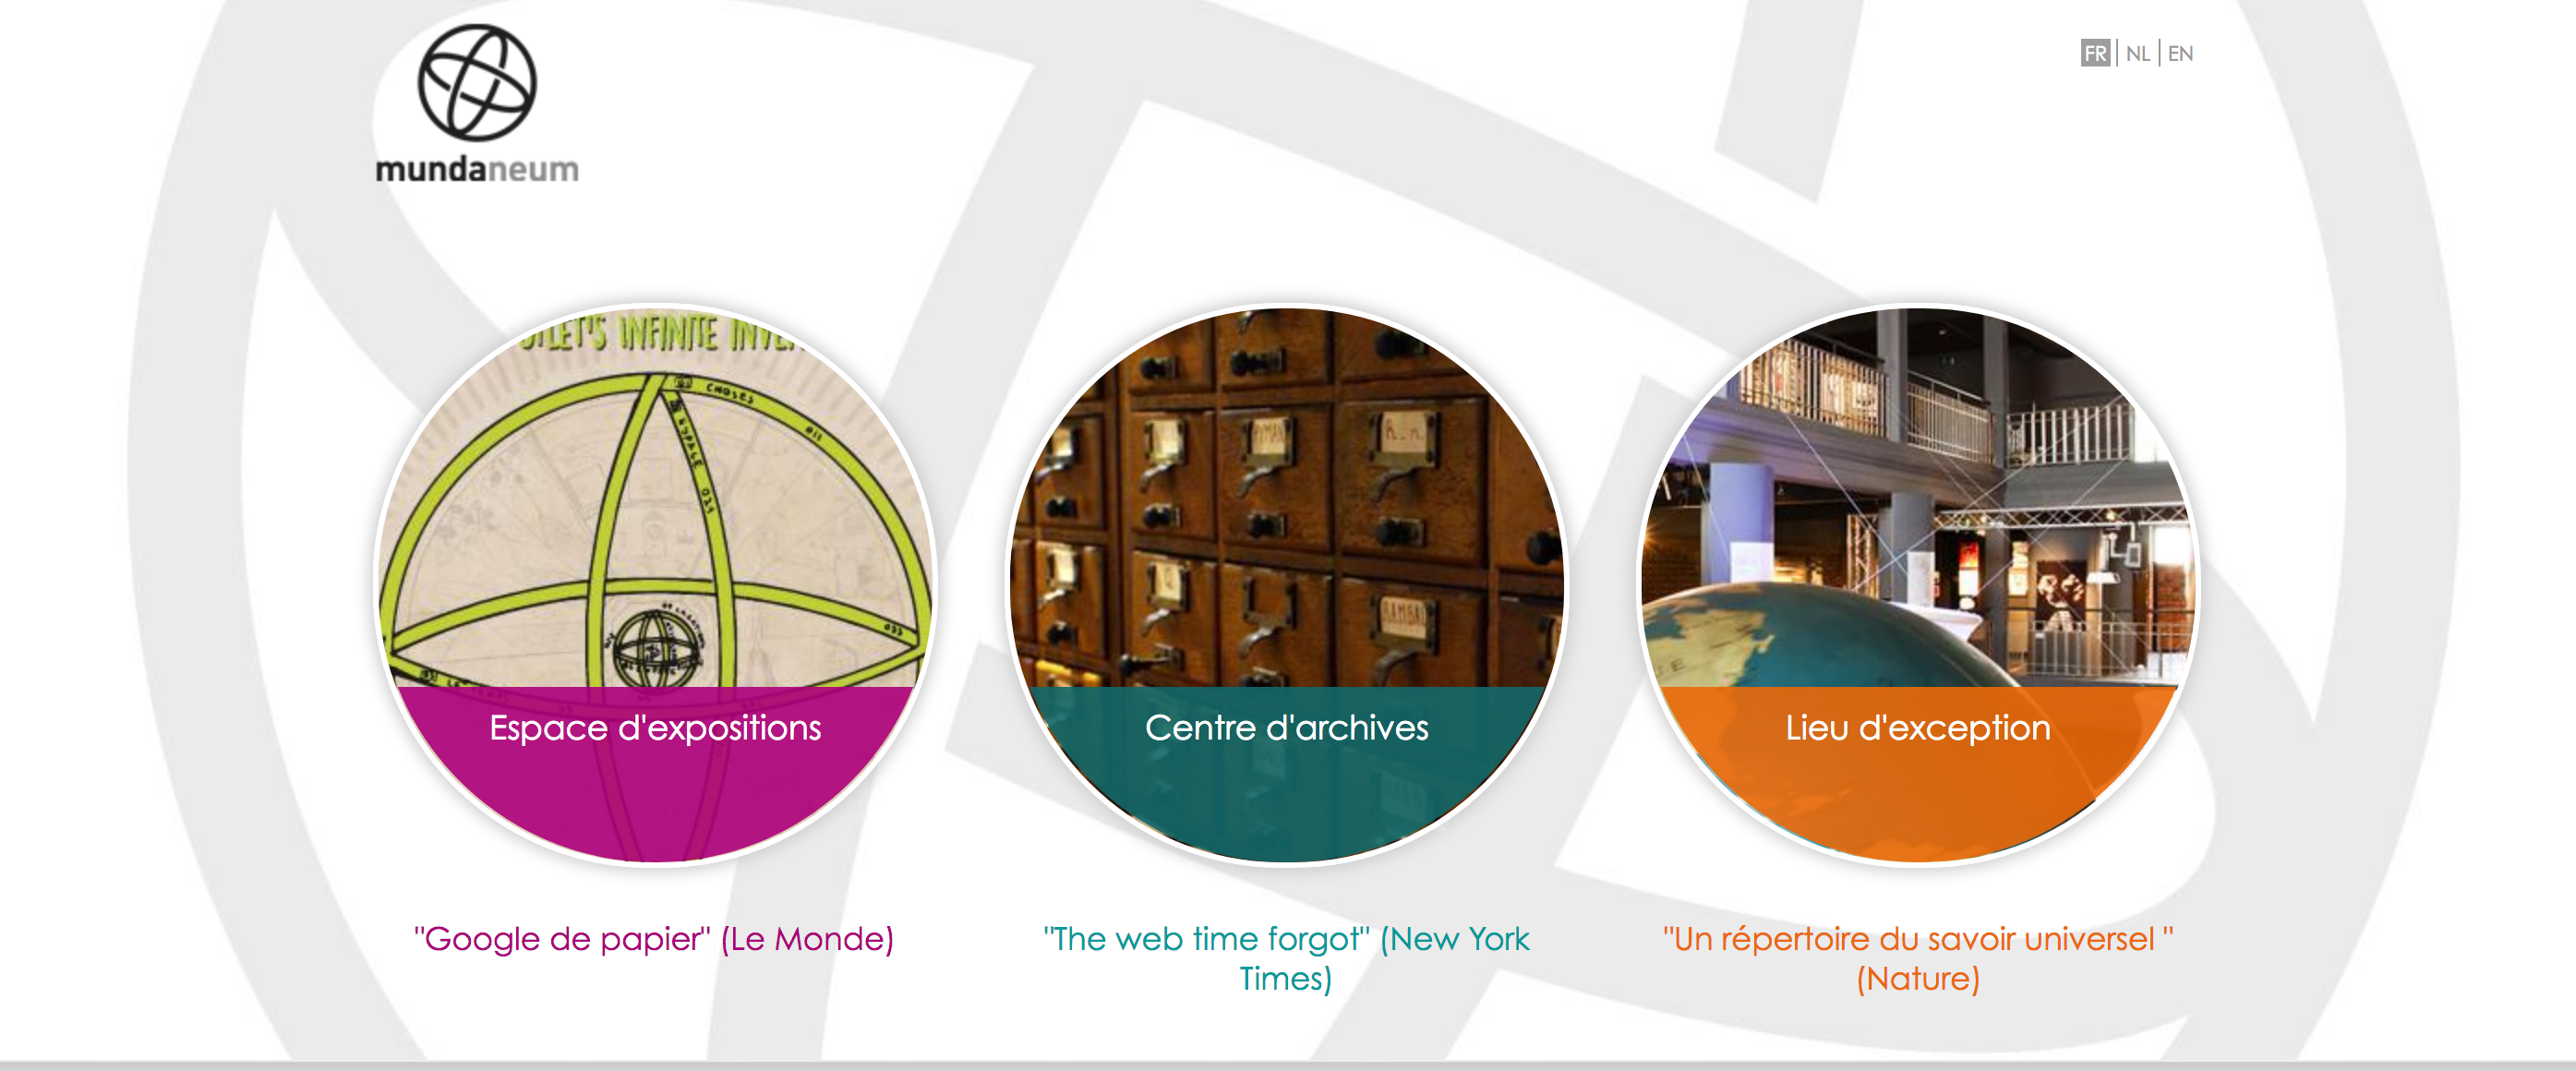
\includegraphics[scale=0.3]{mundaneum}
\caption{Capture-d'écran du site internet du \textit{Mundaneum}.}
\end{figure}

Diverses bibliothèques procèdent parallèlement au \textit{microfilmage} ou numérisation de leurs collections. En 1927, la Librairie du Congrès (États-Unis) procède au microfilmage de quelques trois millions de pages de livres et manuscrits de la \textit{British Library} (Angleterre). Les microfilms générés durant cette grande période de réhabilitation des documents sont encore utilisés aujourd'hui\footnote{\cite[p. 9]{thylstrup_politics_2018}}.

Vannevar Bush\footnote{Vannevar Bush (1890-1974), ingénieur et inventeur américain} décrit son invention le \textit{Memex}, convaincu que les méthodes traditionnelles d'indexation ne suffisent pas à répondre aux besoins des scientifiques modernes\footnote{\cite[p. 11]{xie_discover_2016}}, dans un fameux article publié en 1945, \og \textit{As We May Think} \fg{}. Il définit sans le savoir ce qui constituera nos futurs ordinateurs personnels.

\begin{quotation}
[\textit{Traduction}]
Il s'agit d'un appareil dans lequel un individu peut stocker tous ses livres, fichiers et communications. Cet appareil est mécanisé de façon à pouvoir être consulté avec flexibilité et rapidité. Il est semblable à un élargissement, dans un format réduit, de la mémoire de l'individu.
 \footnote{\inquote{\textit{[It is] a device in which an individual stores all his books, records, and communications, and which is mechanized so that it may be consulted with exceeding speed and flexibility. It is an enlarged intimate supplement to his memory}}\cite[p. 6]{weiss_using_2014}.}
 \end{quotation}

L'américain Richard Feynman\footnote{Richard Feynman (1918-1988), physicien et théoricien américain, précurseur en nanotechnologies.} conçoit dès 1959 les perspectives offertes par les nouvelles technologies et leurs potentiels impacts sur les pratiques des bibliothécaires et autres spécialistes de l'information. Sa conférence \emph{There's plenty of room at the bottom} donnée le 29 décembre 1959, lors de la réunion annuelle de l'\textit{American Physical Society (California Institute of Technology)} propose de comprimer l'intégralité de l'encyclopédie britannique afin de la réduire à la taille d'une tête d'épingle. Il ira même plus loin en concluant ses propos par la proposition de réduire l'intégralité de la connaissance humaine suivant la même méthode. Il imagine pour cela un système de conversion des caractères textuels en traits et points. Nous sommes un an avant le début des travaux sur l'\gls{ascii}\footnote{Norme étasunienne qui sert comme premier système d'encodage informatique des caractères en anglais et apportera un premier niveau de standardisation. Les caractères utilisés en anglais sont encodés suivant une combinaison de 0 et de 1.}\footnote{\cite[p. 25]{association_pour_le_patrimoine_naturel_et_culturel_du_canton_de_vaud_patrimoine_2012}}.

Dans son ouvrage \emph{Libraries of the Future}, paru en 1965,  J.C.R. Licklider\footnote{Joseph Carl Robnett Licklider (1915-1990), psychologue et informaticien américain.} propose d'étendre le monde des bibliothèques à celui des ordinateurs. Au-delà de l'objet livre, présenter faits et idées en fonctions, classes d'informations et domaines de connaissances, \inquote{\textit{[engineers] need to substitute for the book a device that will make it easy to transmit information without transporting material, and that will not only present information to people but also process it for them\footnote{\cite[p. 6]{weiss_using_2014}}.}} Il faudra encore plus d'une génération pour que le numérique soit pleinement appliqué à la gestion des livres et du contenu informationnel qu'ils contiennent.

Nous concluons cette section par le projet Gutenberg, lancé par Michel Hart\footnote{Michael Stern Hart (1947-2011), auteur américain et inventeur du livre électronique ou \textit{e-book.}} en 1971. Convaincu que la valeur ajoutée des ordinateurs ne se trouve pas uniquement dans leur puissance de calcul, mais également dans leur capacité à stocker et à retrouver des informations, il parvient à rassembler une équipe de volontaires pour saisir au clavier des textes libres de droit dans un format accessible et compréhensible par les ordinateurs : une version basique de l'\gls{ascii}. Ces textes analogues ainsi convertis dans une forme numérique sont conservés sur un serveur en mode texte, et diffusés auprès des membres du réseau \textit{ARPAnet\footnote{\textit{Advanced Research Projects Agency Network}, réseau qui a servi de modèle à notre actuel internet.}}\footnote{\cite[p. 10]{association_pour_le_patrimoine_naturel_et_culturel_du_canton_de_vaud_patrimoine_2012}}. L'objectif n'est alors pas la précision, mais une plus ou moins haute correspondance entre texte écrit et rendu numérique\footnote{\cite[p. 10]{thylstrup_politics_2018}}. Ce projet peut être perçu comme le premier projet de bibliothèque numérique, alors que l'internet et le web que nous connaissons aujourd'hui ne seront mis en place que dans les années 90.

\newpage
\begin{figure}[H]% force à placer l'image au sein de notre balise figure
\centering
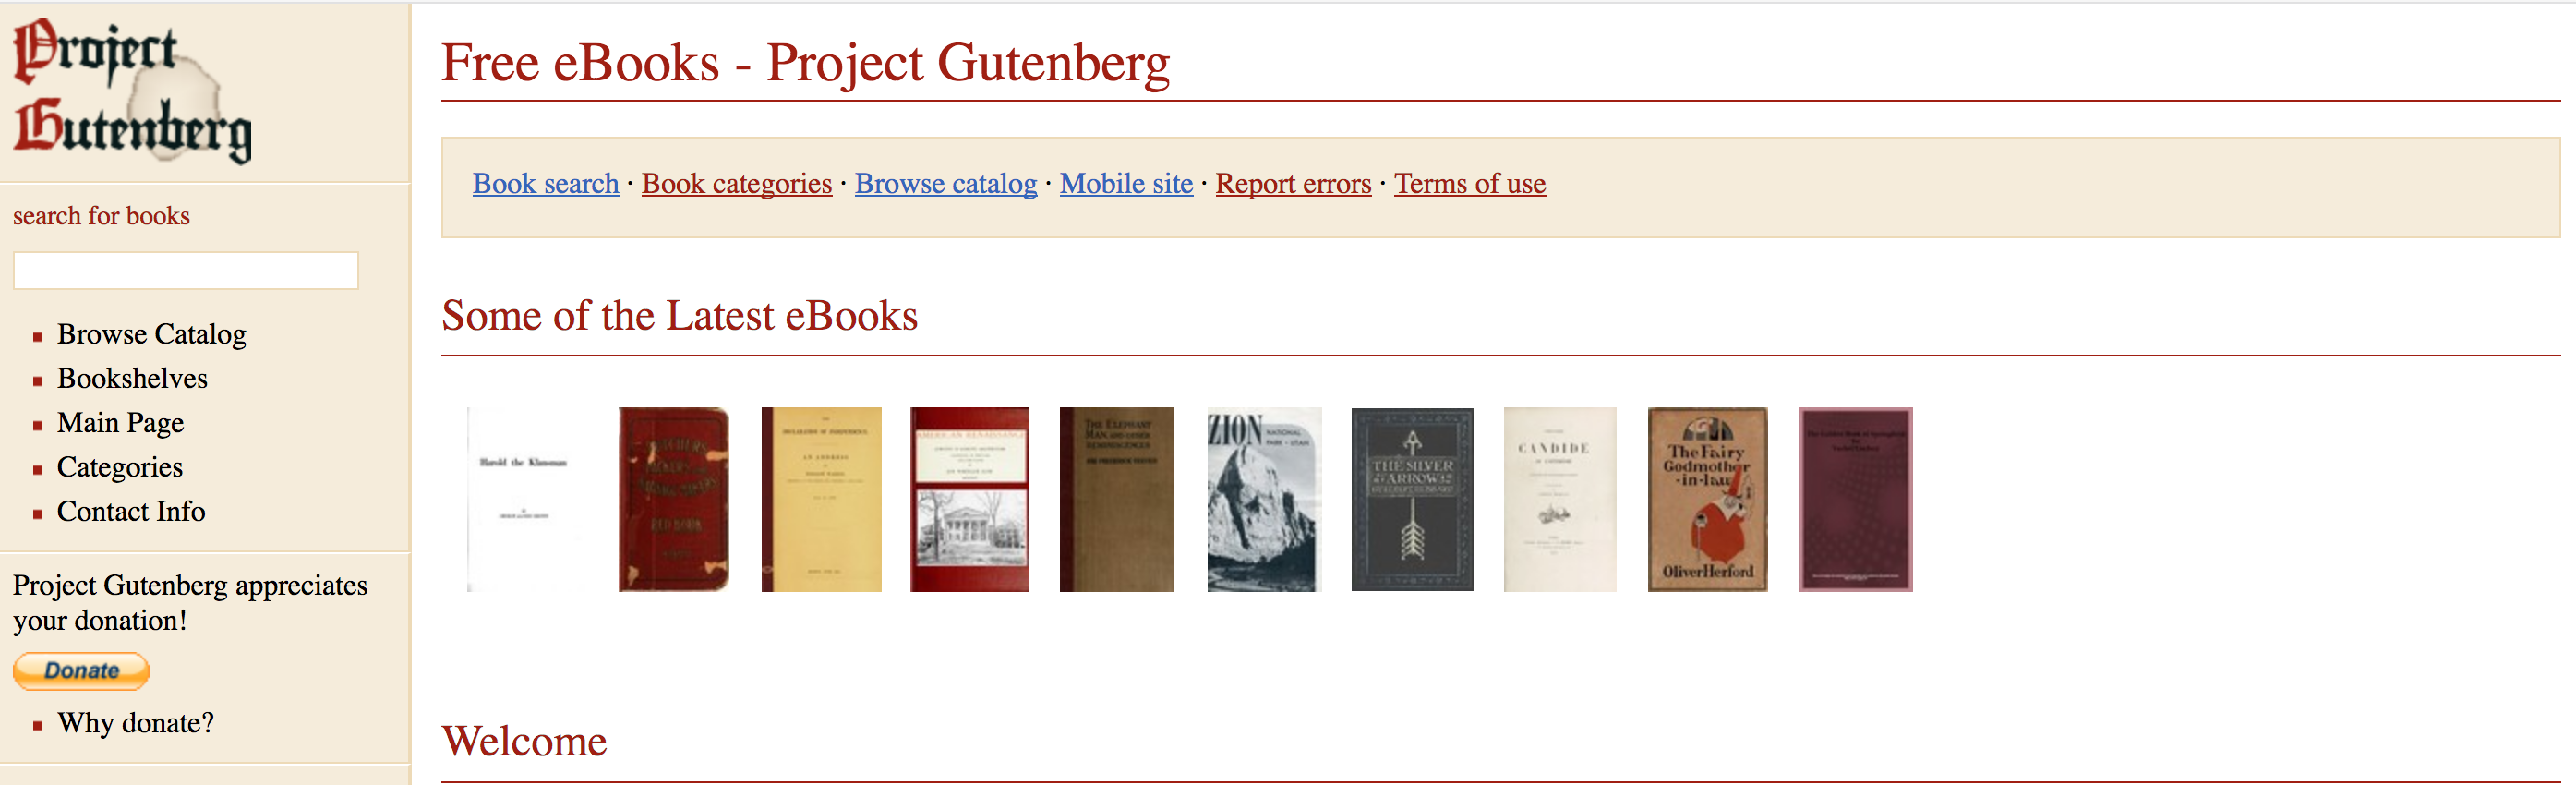
\includegraphics[scale=0.33]{projet_gutenberg}
\caption{Capture-d'écran du site internet du \textit{Projet Gutenberg}.}
\end{figure}

Les principaux défis techniques permettant le passage d'un texte physique à une version numérique sont levés entre 1970 et 1990 (le coût des scanners devient abordable pour les bibliothèques, les formats des images digitales se normalisent, l'industrie des logiciels s'intéresse aux programmes de \gls{reo})\footnote{\cite{association_pour_le_patrimoine_naturel_et_culturel_du_canton_de_vaud_patrimoine_2012}}. 

Désormais les écrans et les claviers servent d'interface entre hommes et ordinateurs, la puissance informatique a été augmentée et les premiers systèmes de recherche documentaires voient le jour\footnote{\cite[p. 10]{weiss_using_2014}}. Pour plus de détails sur ces développements du matériel informatique, liés à l'avènement d'internet\footnote{L'ensemble des supports de cours élaborés par Mr. Philippe Bootz, dans le cadre du cours "Sémiotique du numérique", suivis durant ma première année de Master en \textit{Humanités numériques : enjeux et technologies}, Université Paris 8, ont servis à l'élaboration de la synthèse des éléments techniques.}, référez-vous à l'annexe \ref{premisse}. 
\newpage

\begin{figure}[H]% force à placer l'image au sein de notre balise figure
%\centering
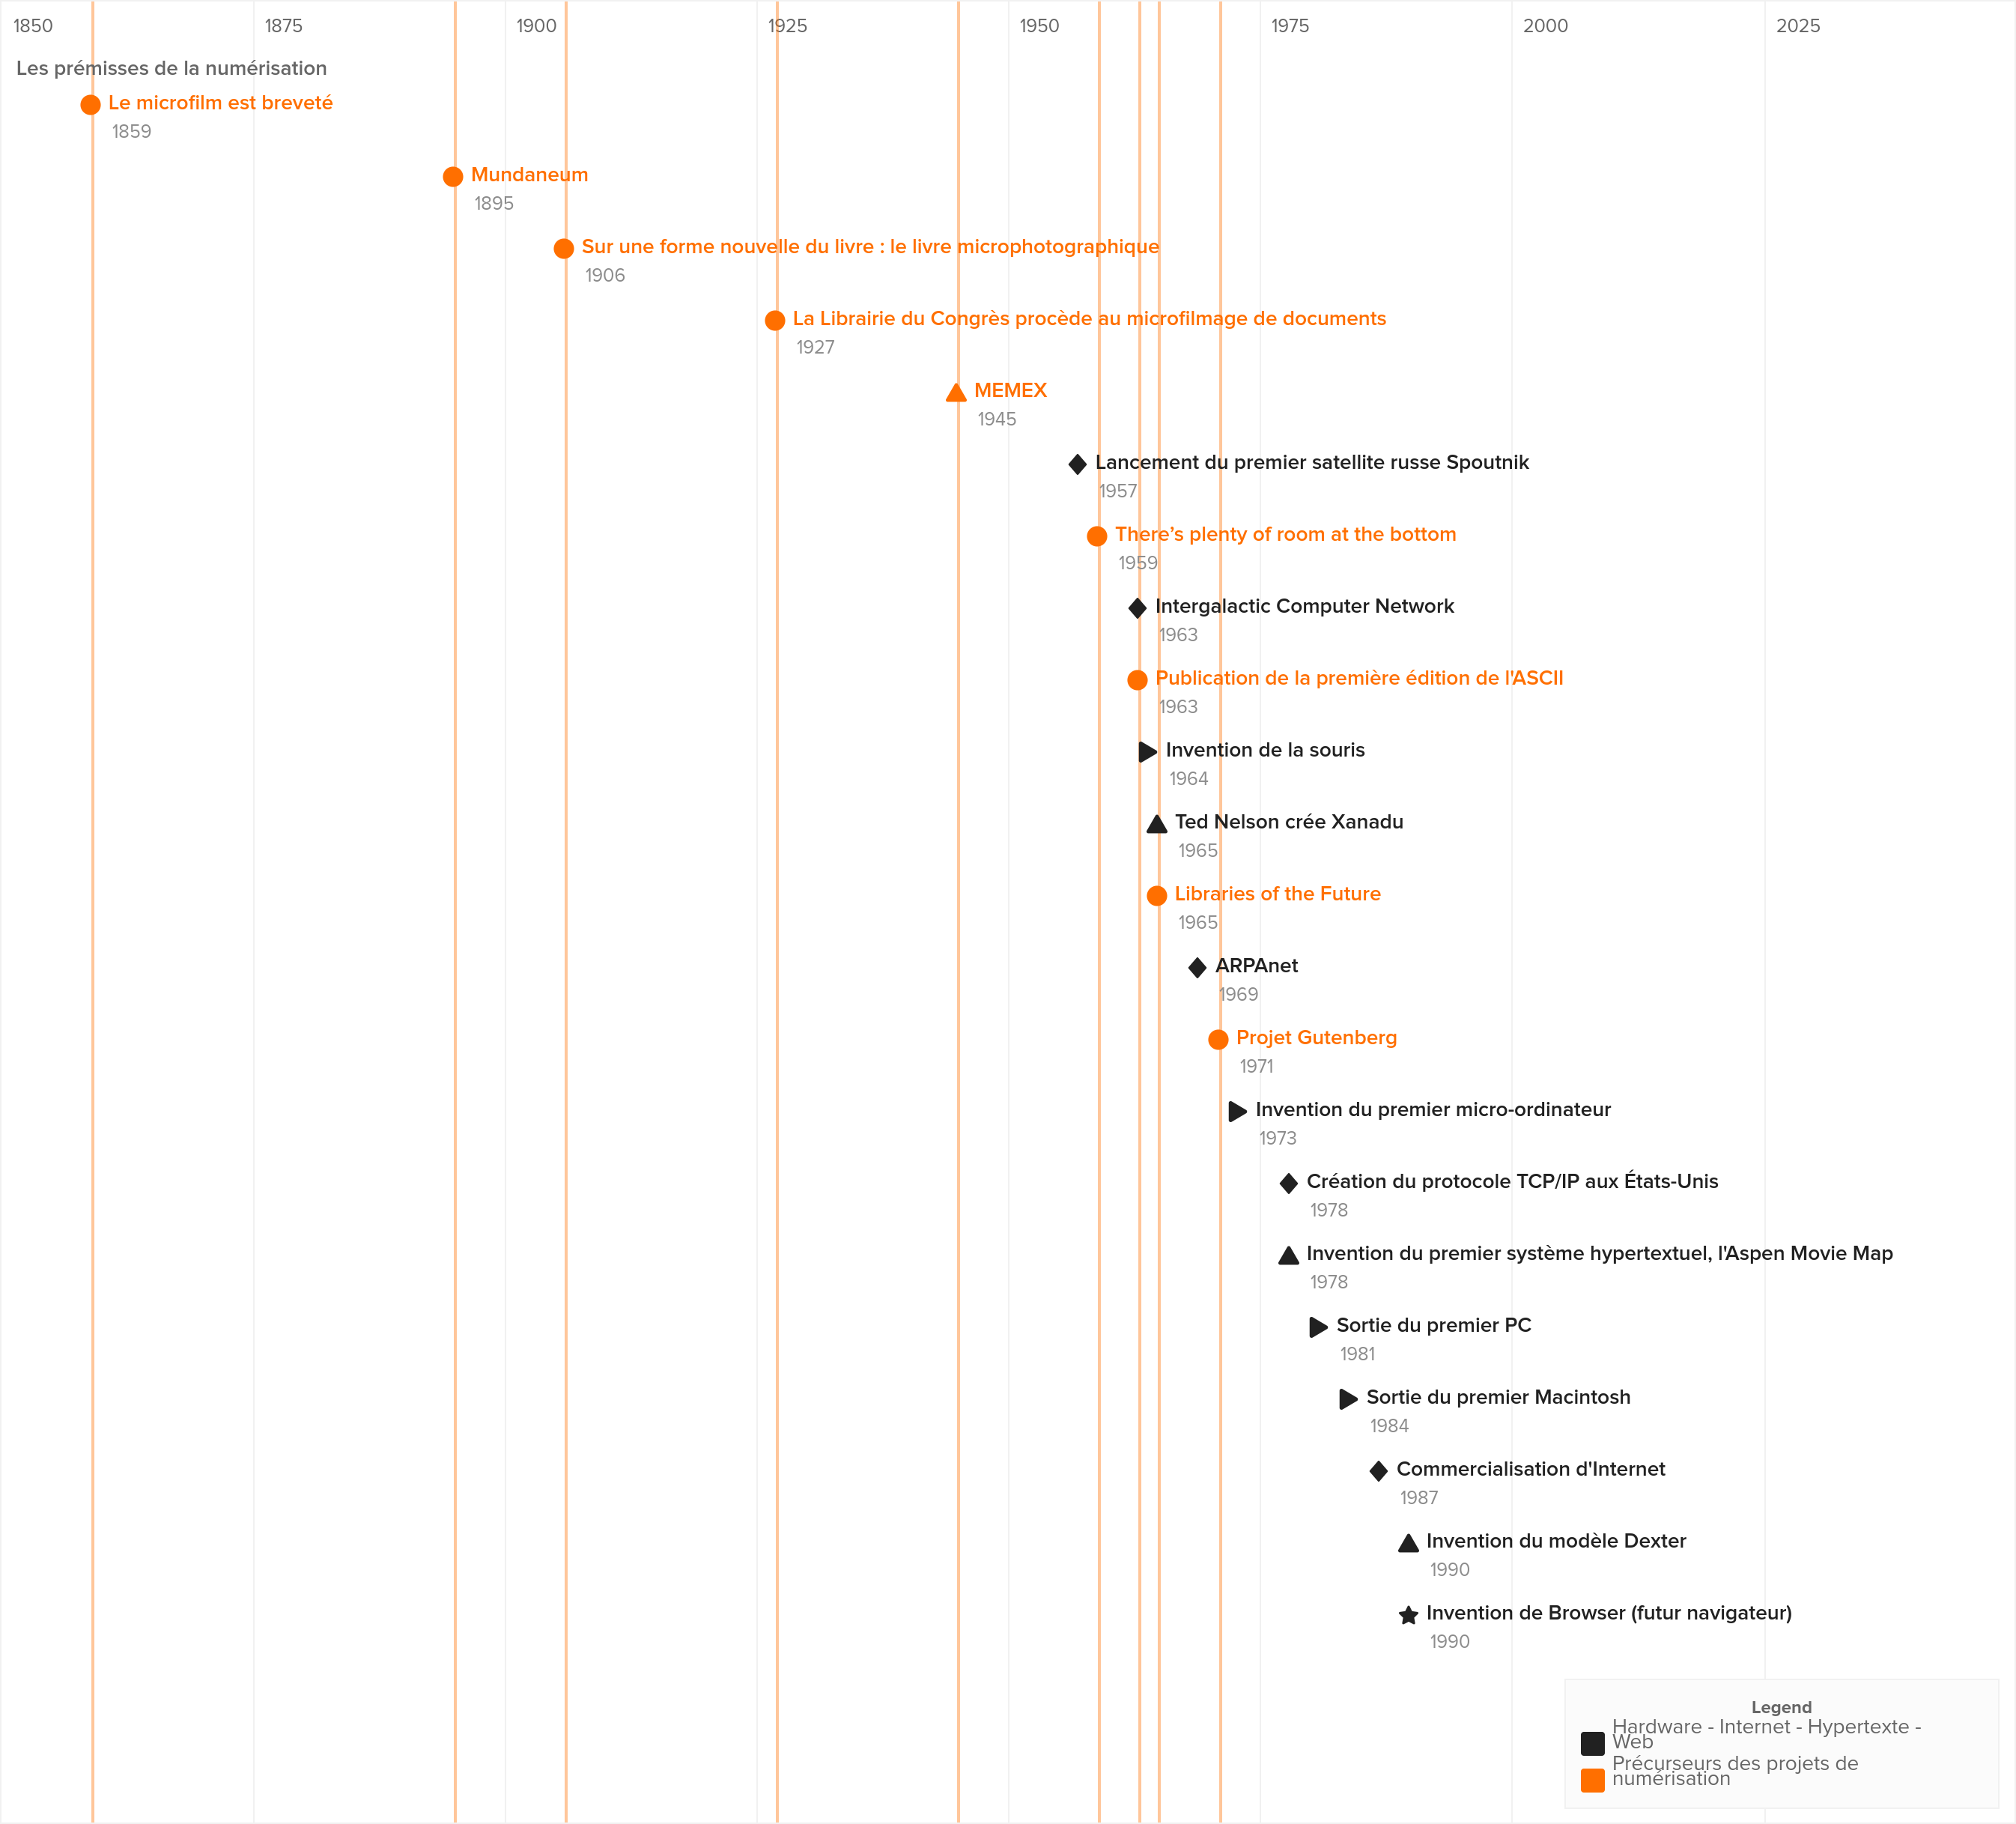
\includegraphics[angle=90, scale=0.21]{premisse_image.png}
\caption{Frise temporelle, \textit{Les prémisses de la numérisation}.}
\end{figure}
\newpage

%========PASSAGE A L'ECHELLE
\section{1990-2000 : Passage à l'échelle}\label{echelle}
%des bibliothèques numériques aux entreprises de numérisation de masse
Bien que les bibliothèques publiques apparaissent dès le milieu du 19\up{e} siècle\footnote{\cite[p.230]{jones_public_2017}}, avec pour vocation de rendre la connaissance accessible à tous, ce n'est qu'au début des années 1990 et l'avènement des ordinateurs personnels, que le mouvement des bibliothèques numériques voit le jour. Au-delà des développements purement techniques, les professionnels réalisent que proposer des collections numériques signifie bien plus que l'acte de \gls{num}, et que le processus est étroitement lié à des enjeux et des controverses culturelles, politiques et légales. Mais comment est-on passé de la bibliothèque numérique, aux projets de numérisation de masse ? 

Nous tenterons dans cette section de proposer une chronologie résumée des faits les plus marquants de cette révolution. Il est important de relever qu'il n'existe pas encore de définition exacte ni de catégorisation pour des projets d'une telle ampleur, et nous avons pu croiser, durant notre état de l'art, les expressions \textit{very large digital libraries} ou \textit{massive digital libraries\footnote{\cite{weiss_using_2014}}} au même titre que \textit{large-scale digitization projects\footnote{\cite[p.47]{lampert_ramping_2018}}\footnote{\cite{yeates_collaborative_2006}}} ou \textit{projets de numérisation de masse}\footnote{\cite{thylstrup_politics_2018}}\footnote{\cite{lampert_ramping_2018}}\footnote{\cite{xie_discover_2016}} pour désigner ces entreprises. Par souci de cohérence et puisque le cadre théorique fait encore débat, nous avons choisi de regrouper toutes les initiatives sous l'appellation de \textit{projets de numérisation de masse}.

Avec la démocratisation de l'ordinateur personnel et la naissance du web, les premières bibliothèques numériques voient le jour. Différents termes servent à les désigner, \textit{electronic library, virtual library, network-accessible libraries, libraries without walls}, reflétant l'évolution du sens de cette expression\footnote{\cite[p.3]{xie_discover_2016}}. D'abord perçues d'un point de vue technique et non comme institution ou objets porteurs d'influences sociales, \inquote{\textit{In this sense, they are an extension and enhancement of information storage and retrieval systems that manipulate digital data in any medium (text, image, sound ; static or dynamic images) and exist in distributed networks}\footnote{\cite[p.243]{jones_public_2017}}}, les bibliothèques numériques garderont trace de ce premier focus technologique\footnote{\cite[p.245]{jones_public_2017}}. 

Karen Calhoun les définit comme un système  de services et de gestion des collections numériques, basé sur une architecture centrée sur les données\footnote{\cite{calhoun_exploring_2014}}.

Prenant conscience des potentialités en termes de services aux utilisateurs, promis par les interfaces numériques, les bibliothèques se mettent à réfléchir au développement de leurs activités, laissant les informaticiens développer les systèmes requis\footnote{\cite{jones_public_2017}}. Les premières entreprises de numérisation sont pensées dans la complémentarité de la mission d'accessibilité de la connaissance humaine, et motivées par les perspectives de préservation de documents rares ou trop fragiles, le rayonnement supplémentaire apporté aux collections et aux institutions par cet accès en ligne, et la possibilité de numériser différents matériaux (photographies, textes, manuscrits etc.)\footnote{\cite[p.274]{lopatin_library_2006}}. Les projets de numérisation héritent toutefois des mêmes biais que les premières collections des bibliothèques publiques, dont les politiques documentaires visaient à élever l'esprit des masses\footnote{\cite{jones_public_2017}}. 

\begin{quotation}
[\textit{Traduction}]
Les programmes de numérisation des bibliothèques ont contribué à la création d'un répertoire de collections spécialisées et de services dédiés à une audience similaire à celle de la bibliothèque physique. Puisque la plupart des bibliothèques engagées dans ces programmes de numérisation sont académiques, les collections sont destinées à un usage d'abord scientifique.\footnote{\inquote{\textit{[...] library digitization programs have largely aimed to establish a repertoire of fairly specialized collections and services targeted at an audience that resembles the host libraries patron base - which, since most digitizing libraries are academics libraries, means designing for scholarly use}}\cite[p.247]{jones_public_2017}.}
\end{quotation}

\begin{quotation}
[\textit{Traduction}]
Les bibliothèques numériques et les bibliothèques publiques se sont aliénées de potentiels utilisateurs en se focalisant trop sur leurs idéaux. Les bibliothèques publiques en traitant de haut les travailleurs et ouvriers, les faisant se sentir indésirables et les bibliothèques numériques en développant des interfaces demandant une connaissance technique, culturelle ou thématique préalable à leur utilisation.
\footnote{\inquote{\textit{[...] both have alienated potential users by holding too strictly to this ideal, public libraries by making factory workers and other laborers feel patronized and unwelcome, and digital libraries by presenting interfaces that require a particular sort of technological, cultural, or domain-specific knowledge in order to use them effectively}}\cite[p.247]{jones_public_2017}.}
\end{quotation}

\textit{The Perseus Digital Library}, est l'un des premiers projets de bibliothèque numérique. Initié en 1985 au sein de l'université Tufts (États-Unis), la version initiale regroupe des textes grecs et leurs traductions anglaises sur un CD-ROM. Le projet évolue vers une première plateforme en ligne en 1995, ouvrant ses collections au monde greco-romain et passant d'un outil d'enseignement à un moteur de recherche. Il rassemble des ressources liées aux études classiques (civilisations grecques et romaines) jusqu'à la renaissance anglaise\footnote{\cite{dubis_web_2003}}.

\begin{figure}[H]% force à placer l'image au sein de notre balise figure
\centering
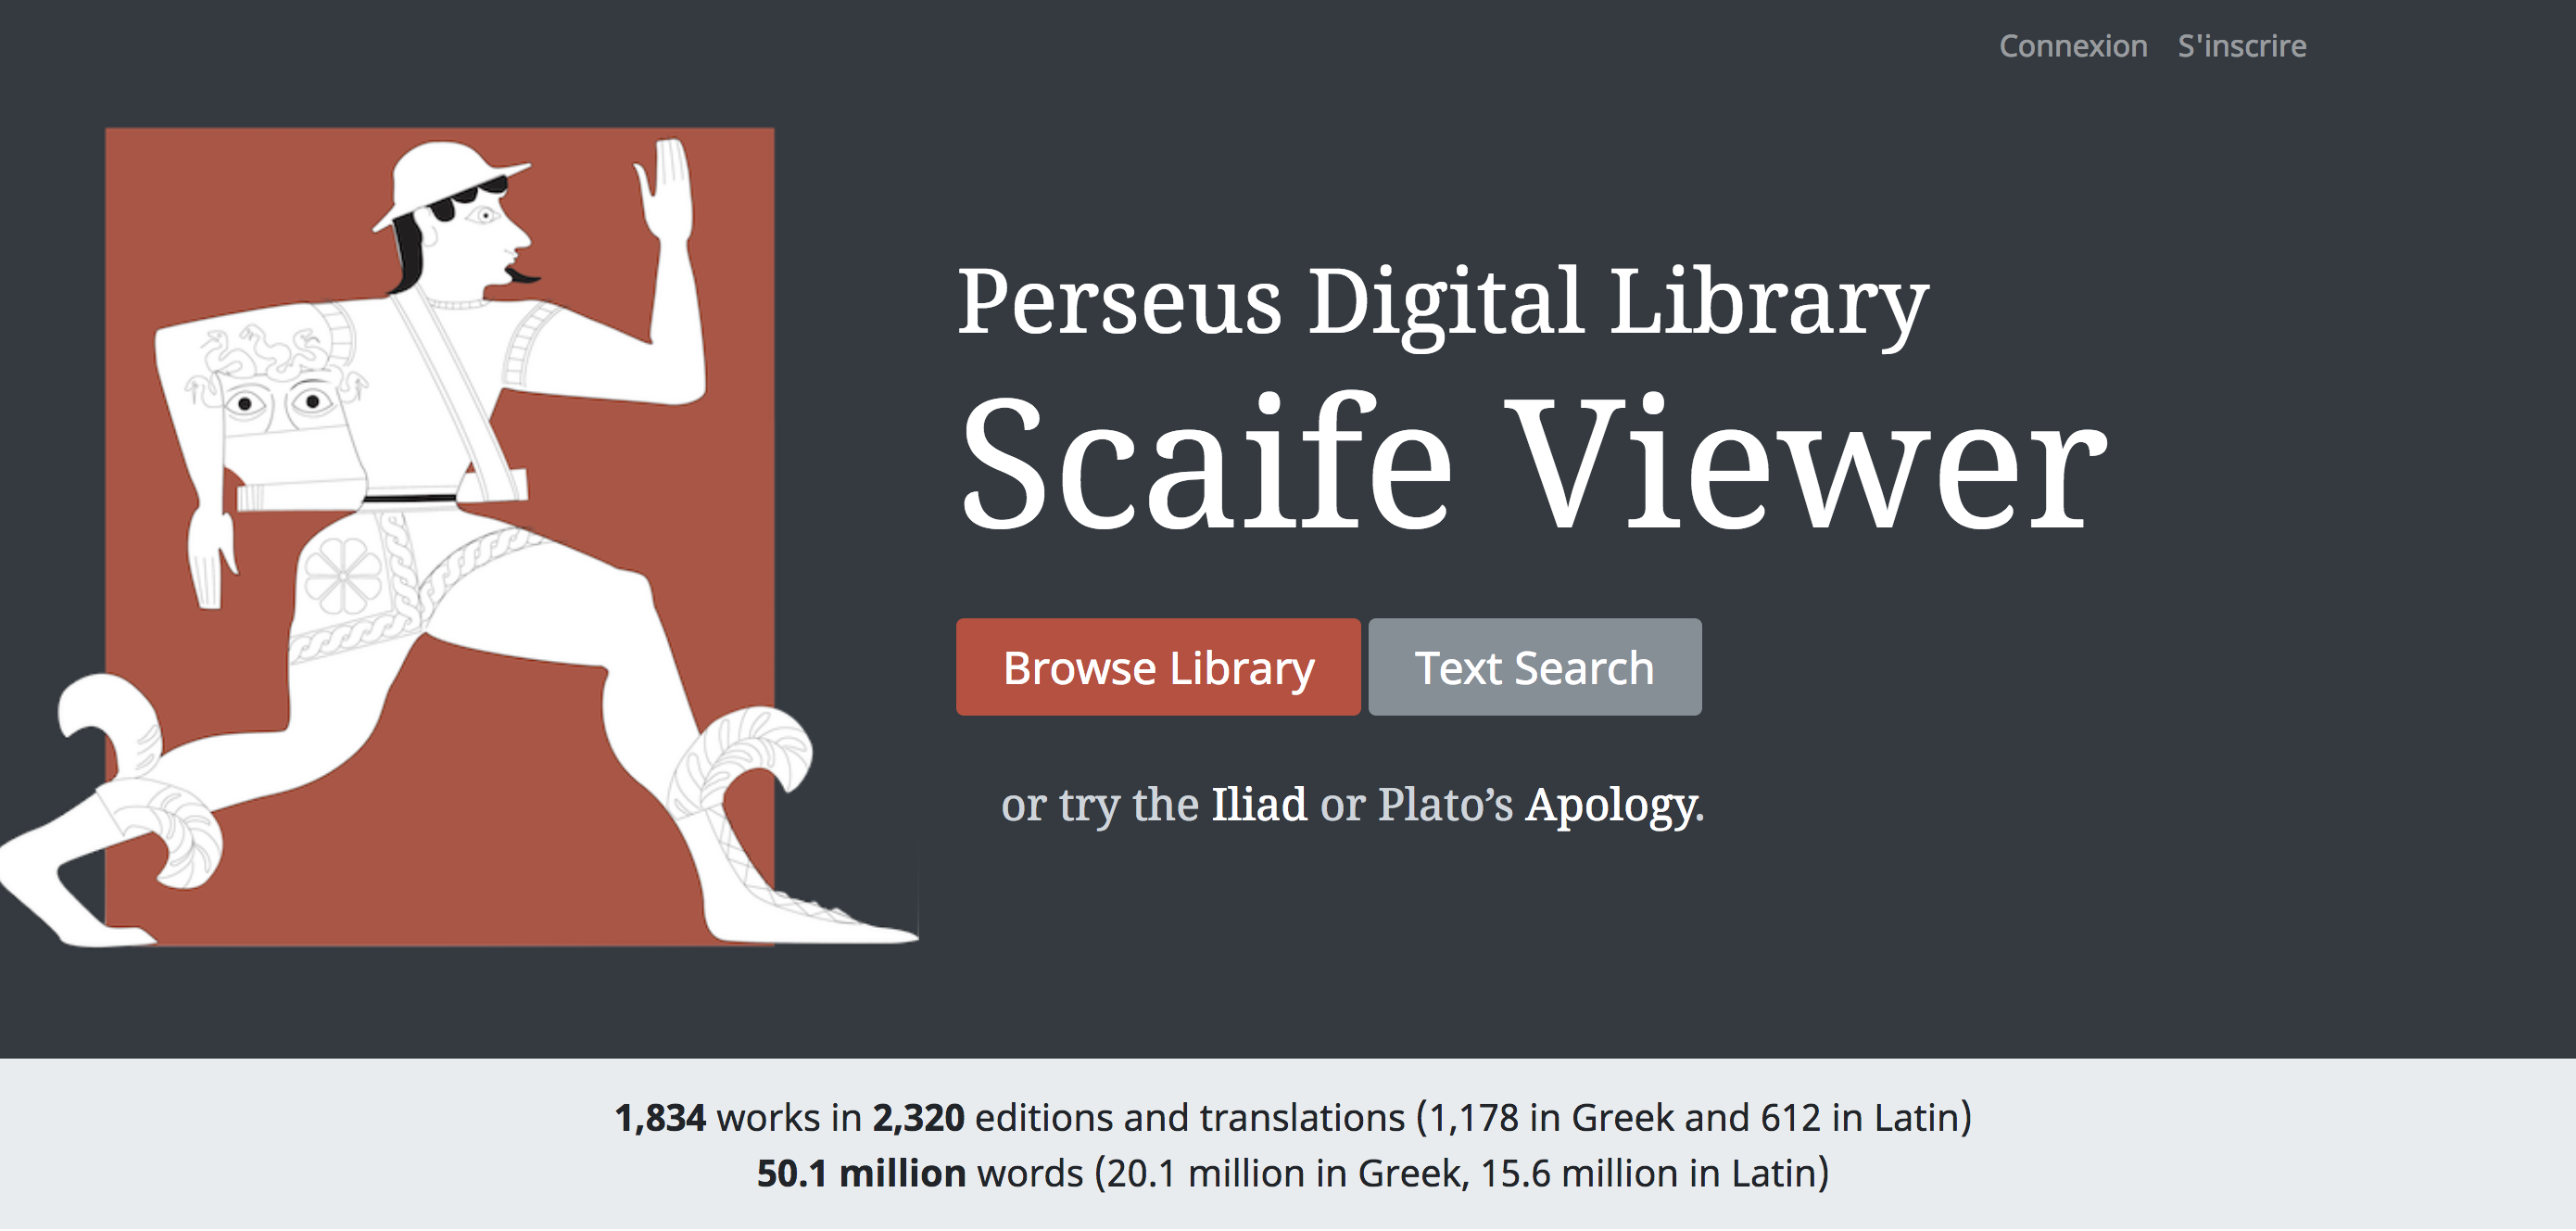
\includegraphics[width=15cm]{perseus}
\caption{Capture-d'écran du visualisateur \textit{Scaife} de la \textit{Perseus Digital Library}.}
\end{figure}

Si ces premières initiatives de numérisation sont ciblées sur une certaine catégorie de collection et vers une audience particulière, c'est pour des raisons de financement. Les institutions culturelles et patrimoniales y voient  une opportunité pour augmenter l'accessibilité de leurs collections et bénéficient dès les premiers temps de fonds publics\footnote{\cite[p.1]{coutts_stepping_2017}}. Les entreprises de numérisation articulent différents champs, nécessitant la création de nouveaux standards et bonnes pratiques, qui mèneront à l'élargissement de la portée de ces projets. 

\begin{quotation}
[\textit{Traduction}]
Il est apparu clairement que c'était un domaine multi-facettes, demandant une uniformisation des processus liés au contenu, aux technologies, à l'infrastructure, à la propriété intellectuelle et à la préservation. Les \gls{glam} ont très vite fait partie des participants les plus enthousiastes. En terme de contenu, les projets à petites échelles sont emblématiques des premières entreprises, se focalisant souvent sur ceux à haute valeur intellectuelle et culturelle. Cependant les activités de cette période visaient en parallèle à la mise en place de standards technologiques, au développement des infrastructures et au déploiement des processus de gestions, de préservation et de respect du droit d'auteur.
\footnote{\inquote{\textit{It also became clear that it was a multifaceted field, requiring that same process to be applied to issues of content, technology, infrastructure, intellectual property and sustainability. Universities, museums, galleries and national libraries were amongst the enthusiastic participants. In term of contents, small-scale projects typified the early work, often showcasing items of major intellectual and cultural value. The activity in this period, however, was as much concentrated on developing experience in and standards for the use of the technology and the provision of infrastructure, legal management and preservation}}\cite[p.12]{coutts_stepping_2017}.}
\end{quotation}

Les premières initiatives de numérisation de masse semblent également issues d'une forme de croyance répandue chez les informaticiens, déclarant que l'information contenue sur le papier deviendrait un jour obsolète, \inquote{\textit{[...] there was an attitude in computer science that putting things on dead trees was obsolete and getting it all into a searchable, digital format was a quest that had to be accomplished someday}\footnote{\cite{cook_googles_nodate}}.} En proposant des livres sous forme numérique, ces pionniers argumentent également qu'ils mettent leurs informations à disposition de tous, utilisant le même motif que pour la création des bibliothèques publiques et reproduisant à nouveau leurs biais\footnote{\cite[p.8]{thylstrup_politics_2018}}.

\begin{quotation}
[\textit{Traduction}]
Tout comme au 19\up{e} siècle, il n'était pas suffisant de laisser le marché proposer des fictions de moindre qualité au peuple sans leur donner accès à des contenus jugés plus pertinents, au 21\up{e} siècle, il n'est pas suffisant de laisser les chercheurs errer sur internet face à un océan de sites, où le meilleur de la connaissance - naturellement contenu dans les livres - n'est pas accessible.
\footnote{\inquote{\textit{Just as in the nineteenth century, it was not seen as sufficient to let the market provide cheap paperback fiction for the masses without giving them access to higher quality materials, in the twenty-first century it is not enough to leave Internet searchers to their own devices in a sea of websites where the best knowledge - that contained in books - is nowhere to be found}}\cite[p.254]{jones_public_2017}.}
\end{quotation}

Le premier projet de numérisation massive répertorié en France est un véritable précurseur et apparaît au tout début des années 90, il découle de la création de la \gls{bnf} en 1989. À la demande du Président François Mitterand, Alain Giffard\footnote{Alain Giffard est directeur du groupement d’intérêt scientifique « Culture-médias \& numérique. » Il a été directeur informatique de la Bibliothèque de France, directeur adjoint de l’Institut Mémoires de l’édition contemporaine (Imec), conseiller technique de la ministre de la Culture et de la Communication pour la société de l’information et président de la mission interministérielle pour l’accès public à l’internet.} est prié d'utiliser les dernières innovations technologiques pour rendre accessible les ouvrages du catalogue de la \gls{bnf} et créer ainsi une très grande bibliothèque. Le projet conduira à la numérisation de 70'000 à 80'000 titres. Pour choisir quels ouvrages numériser, il n'eut pas recours à des bibliothécaires mais à des scientifiques et écrivains, ce qui fut possible car le projet était directement lié au Président. Alain Giffard explique d'ailleurs qu'il a personnellement acheté un grand nombre des livres à numériser, puisqu'ils n'étaient pas dans les collections de la \gls{bnf}, et que celle-ci avait du mal à collaborer avec ce projet. Cet exemple illustre bien le fait que les projets de numérisation massive, au-delà des enjeux techniques, sont aussi des questions politiques qui soulèvent des débats de territorialité (institutionnelle ou nationale), matérialité et culture\footnote{\cite[p.11]{thylstrup_politics_2018}}.  

Ces documents numérisés seront intégrés en 1997 au projet plus connu de numérisation massive, \textit{Gallica}. Ce projet, également mandaté par le Président François Mitterand, vise à numériser les livres libres de droit issus des collections de la \gls{bnf}, depuis le Moyen-Âge jusque vers 1930, avec une priorité pour les documents illustrant la culture francophone. Environ quatre millions de documents sont disponibles sur la plateforme du projet\footnote{\cite[p.140]{thylstrup_politics_2018}}.

\begin{figure}[H]% force à placer l'image au sein de notre balise figure
\centering
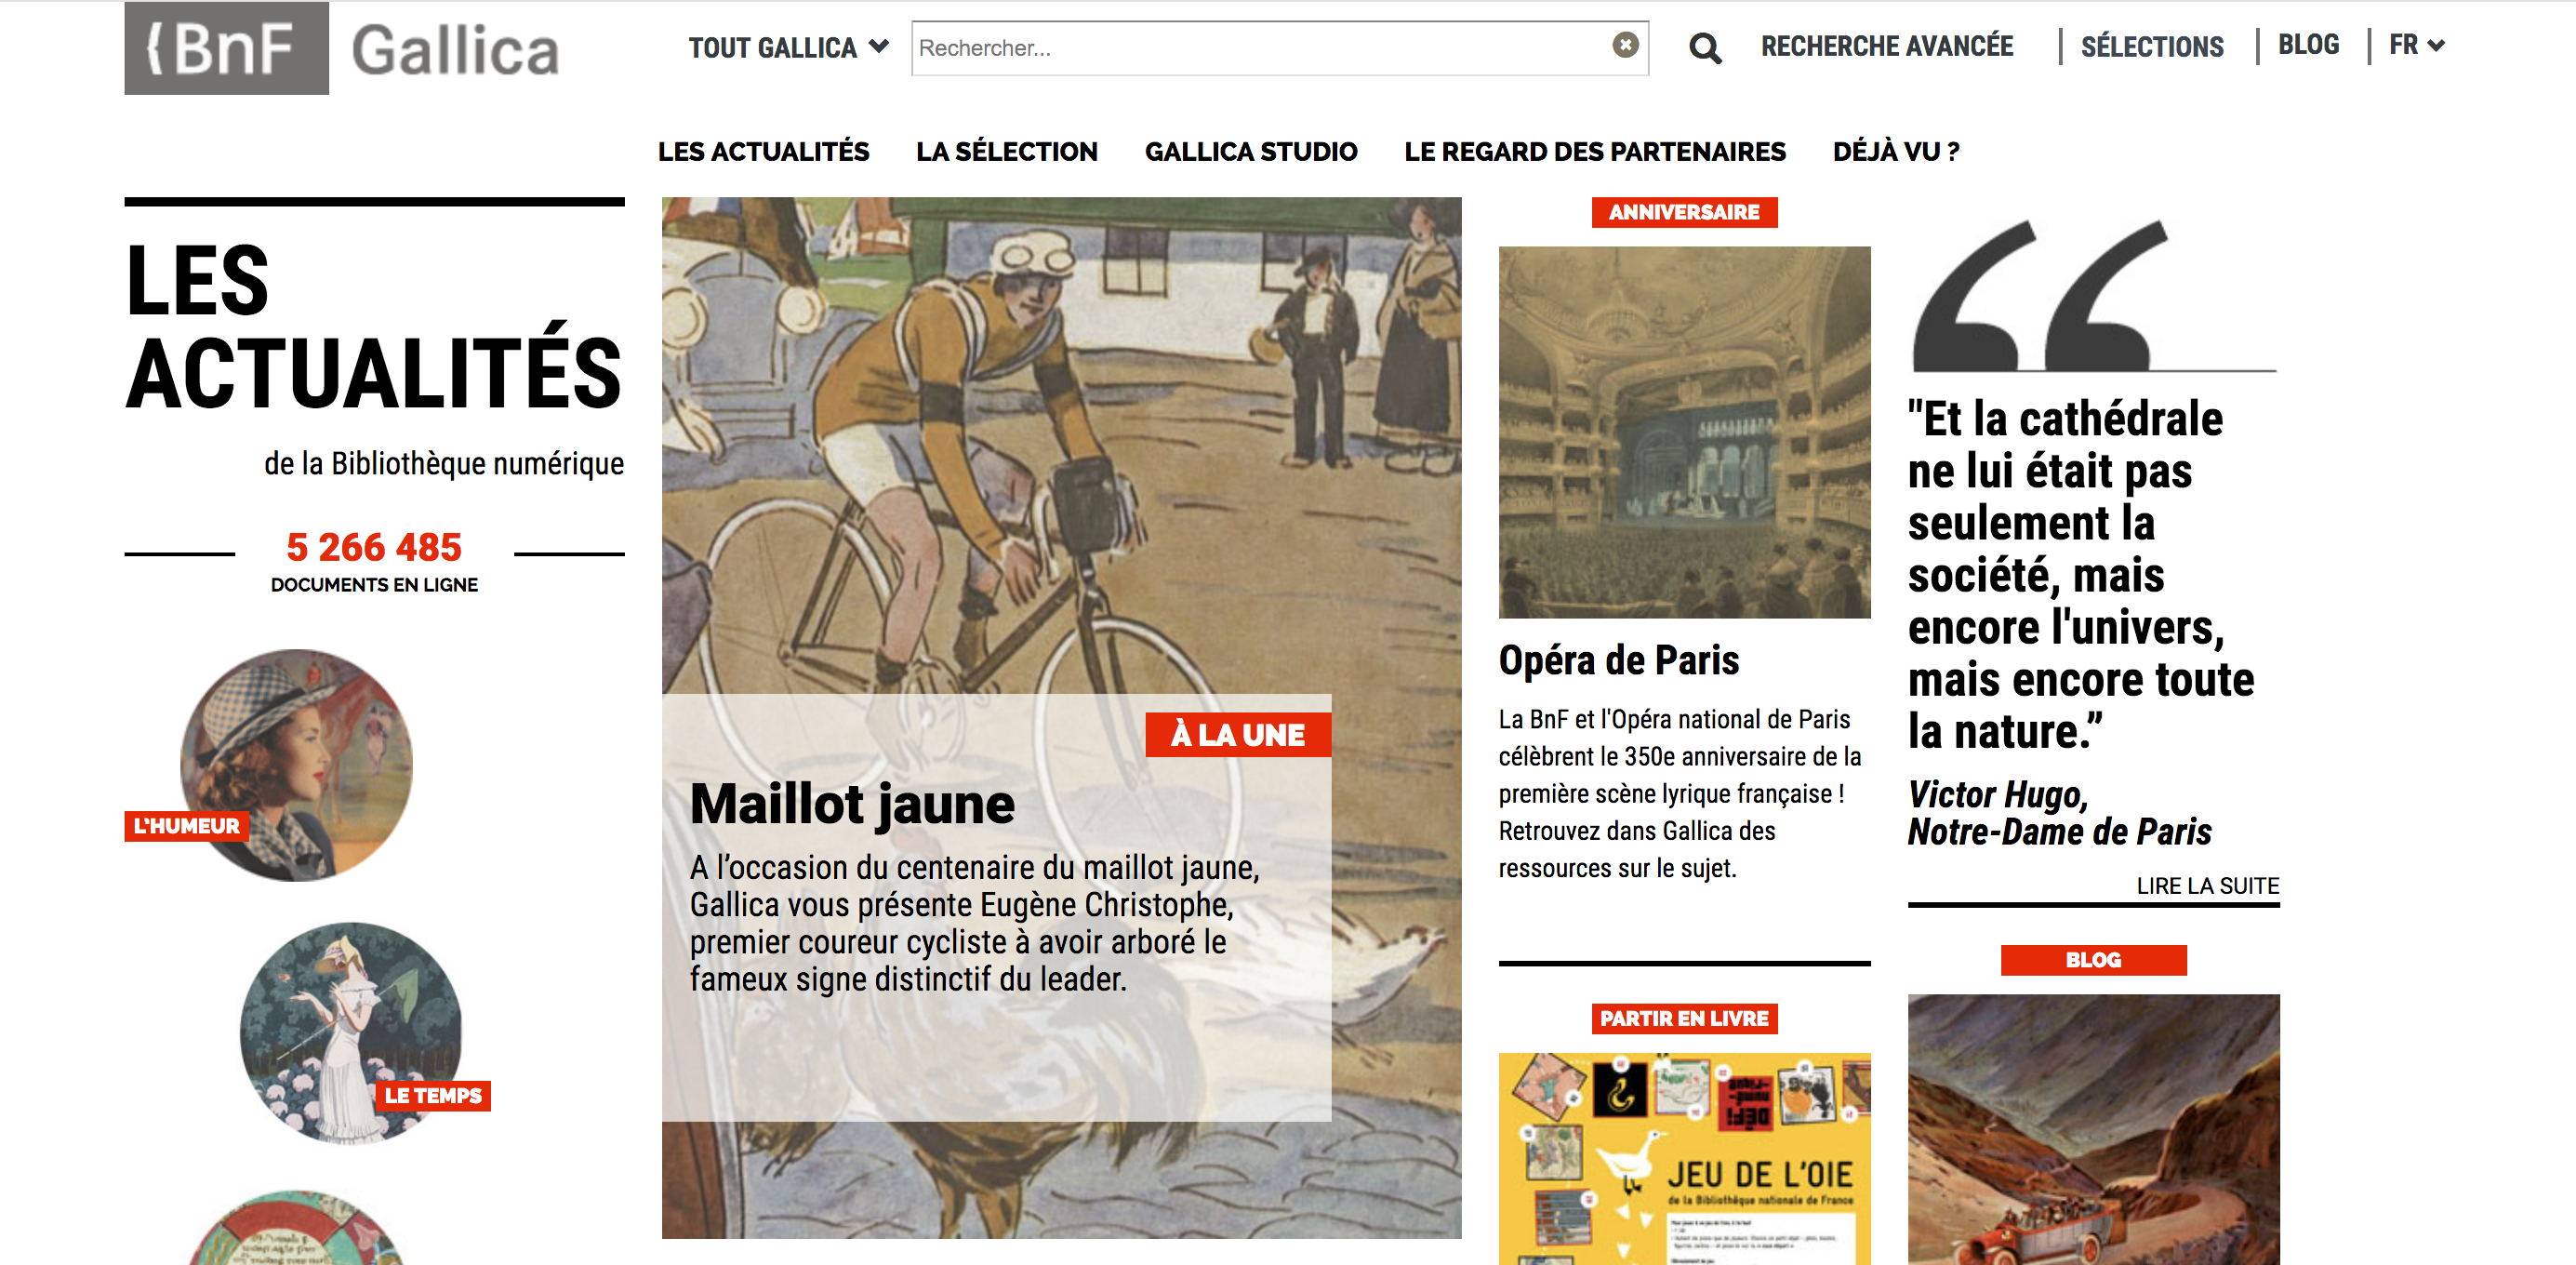
\includegraphics[width=15cm]{gallica}
\caption{Capture-d'écran de la plateforme du projet \textit{Gallica}.}
\end{figure}
L'\textit{Universal Digital Library} est initiée en 1995 par différents scientifiques en partenariat avec la Canergie Mellon Foundation (États-Unis). En 1998, ce projet est à l'origine du \textit{Thousand Book Project} qui sera finalement augmenté jusqu'à devenir le \textit{Million Book Project}, successivement terminé en 2007. Il se distingue des autres projets de numérisation de masse, en incluant dès le départ des institutions chinoises, indiennes ou égyptiennes. L'entreprise de numérisation s'est toutefois terminée en 2008\footnote{\cite[p.12]{thylstrup_politics_2018}}, et la plateforme du projet n'est pas parfaitement maintenue. Cet exemple, pourtant ambitieux, démontre que l'avenir réservé à de nombreux projets de numérisation est toujours bien incertain\footnote{\cite[p.12]{weiss_using_2014}}. Andrew Weiss appelle à une meilleure caractérisation des projets de numérisation de masse, afin d'en préserver l'accessibilité sur le long-terme et à sortir de tels projets des contraintes du marché économique : \inquote{\textit{However, in dealing with consortia of public and nonprofit educational institutions, market forces should not be the sole factor determining their overall sustainability, especially when the content is of significant cultural and social value\footnote{\cite[p.30]{weiss_using_2014}}.}}

\begin{figure}[H]% force à placer l'image au sein de notre balise figure
\centering
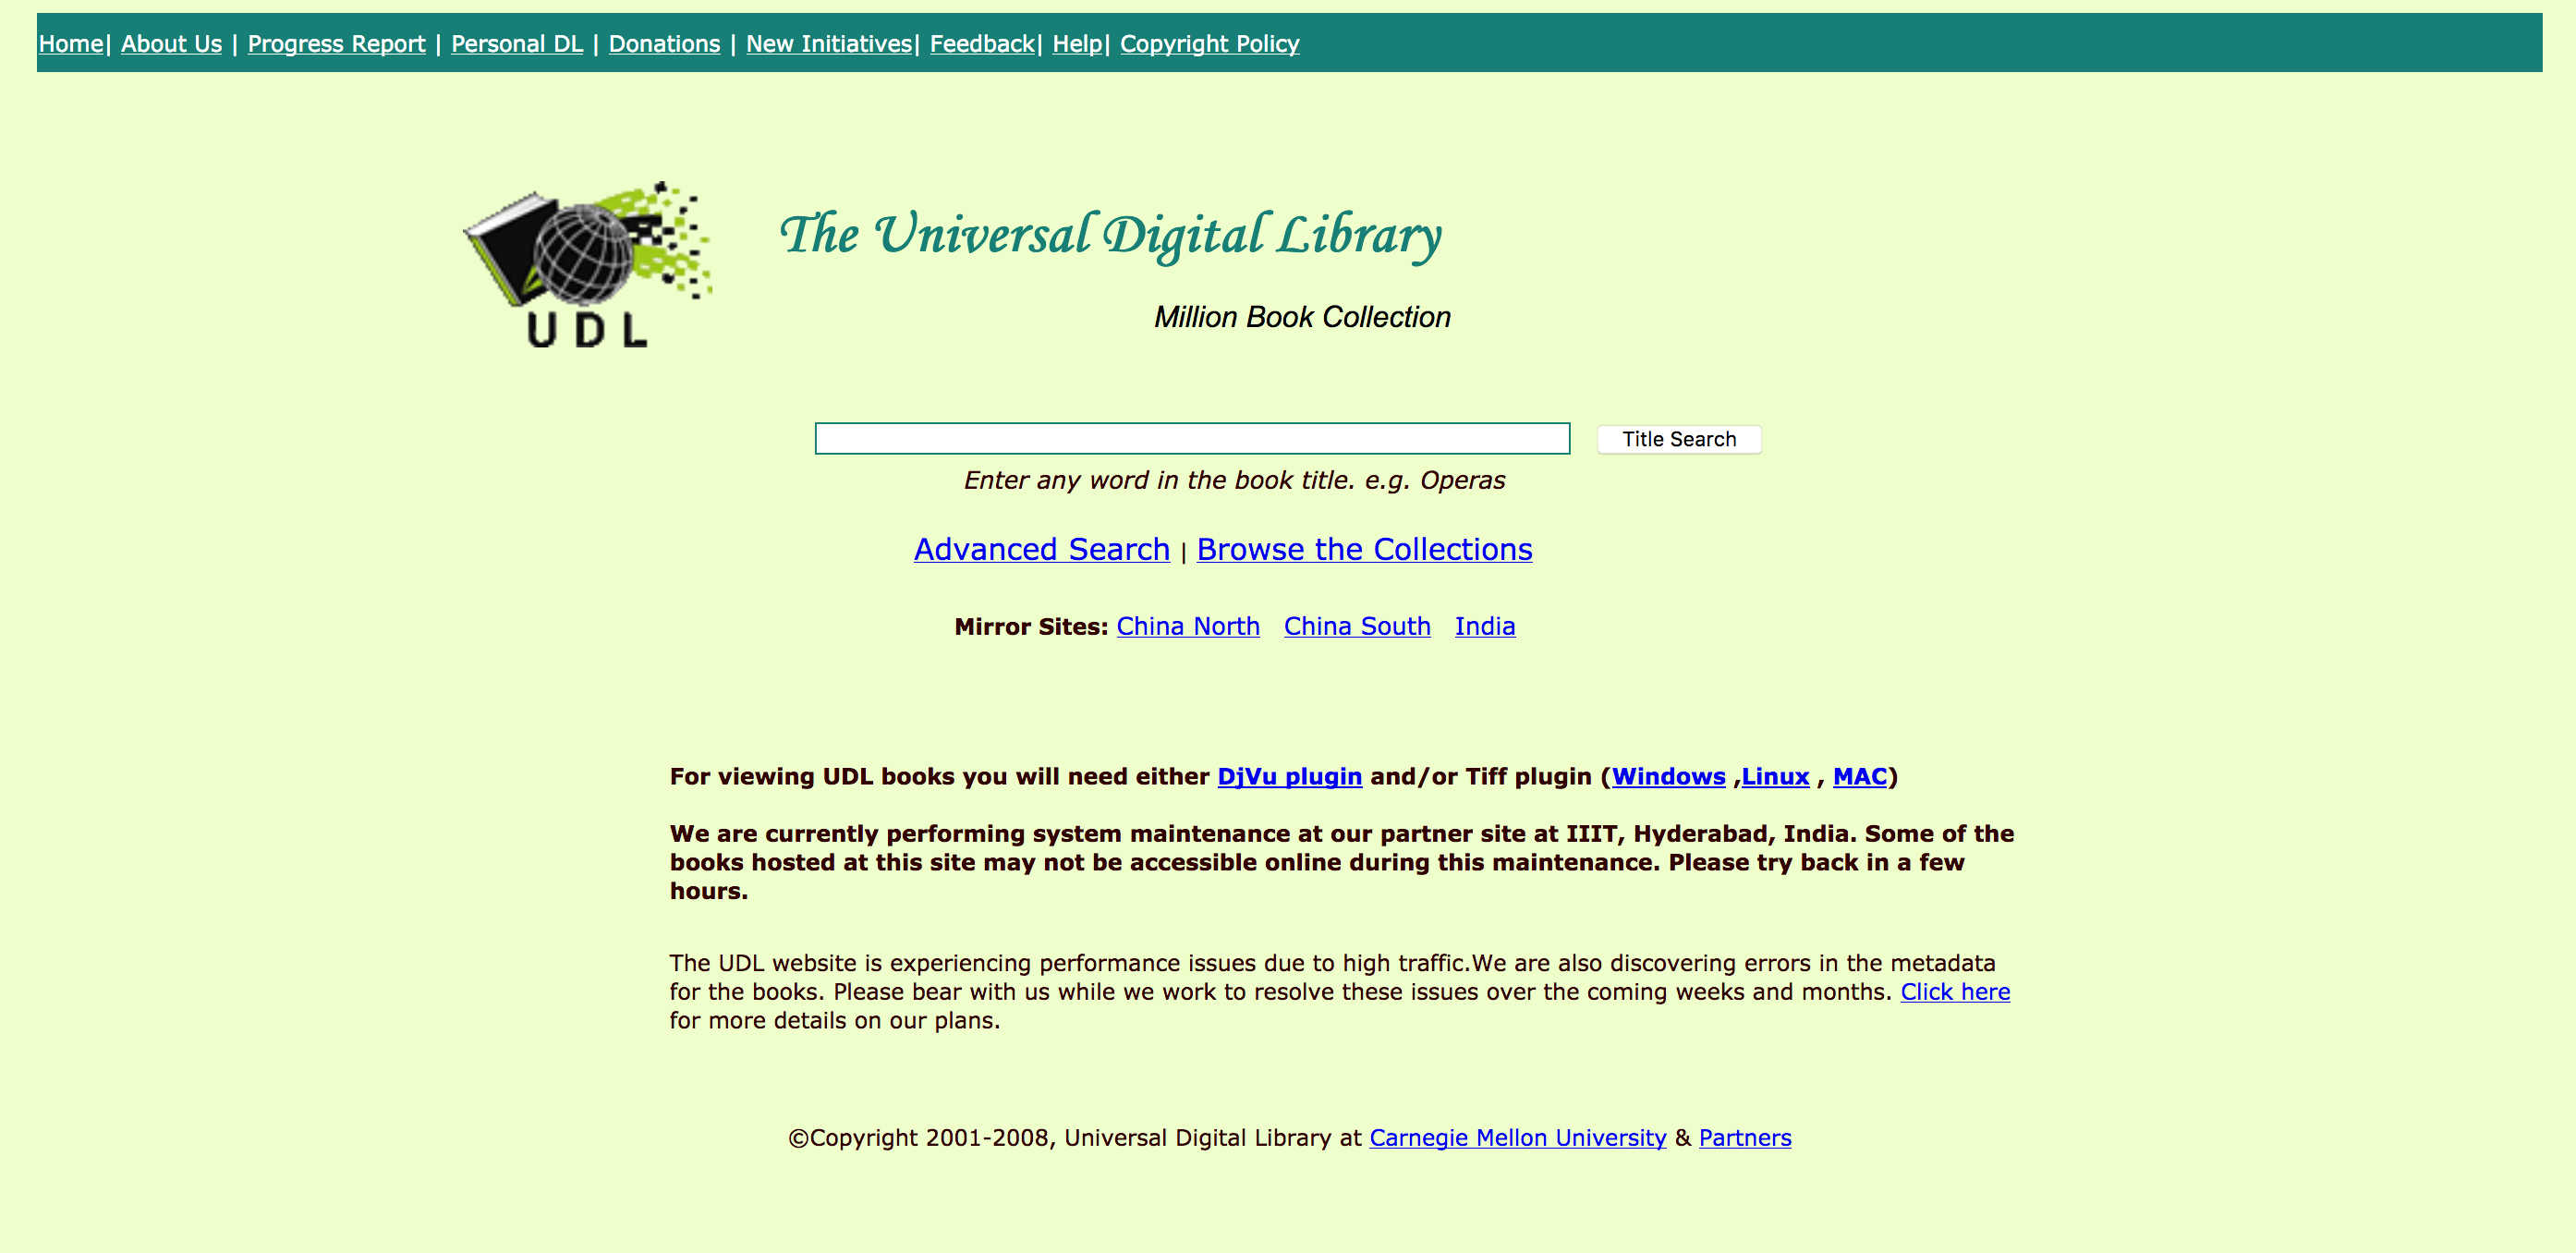
\includegraphics[width=15cm]{udl}
\caption{Capture-d'écran de la plateforme du projet \textit{Universal Digital Library}.}
\end{figure}

1996, marque également le lancement d'un projet se poursuivant aujourd'hui : \textit{The Internet Archive}. Fondé par l'activiste du \gls{oa} Brewster Kahle, avec pour objectif initial de préserver le matériel né numériquement (à l'instar des pages et des sites web). Le projet finira par numériser des livres dès 2005, avec l'aide d'une infrastructure regroupant de grandes institutions patrimoniales et acteurs privés, \textit{The Open Content Alliance}\footnote{\cite[p.12]{thylstrup_politics_2018}}.

Dans leur désir d'accessibilité, les projets de numérisation de masse ne tiennent d'abord pas compte des aspects légaux propres aux ouvrages numériques\footnote{\cite[p.251]{jones_public_2017}}, et se voient imposer un certain nombre de restrictions à ce désir d'ouverture. Toutefois l'ambition de construire une bibliothèque numérique universelle commence à se répandre, notamment au sein de l'entreprise Google\footnote{\cite{cook_googles_nodate}}. Il est important de spécifier qu'au début des années 2000 de nombreux standards et  bonnes pratiques ont été définis et ouvrent la voie aux futurs projets\footnote{\cite{dunning_digitising_2009}} : \inquote{\textit{The digital lifecycle is now well defined, moving from creation through curation, preservation, discovery and use to the creation of new knowledge and content\footnote{\cite[p.245]{jones_public_2017}}.}} Le mouvement des bibliothèques numériques va continuer de s'amplifier avec de nouveaux projets de numérisation de masse et l'apparition des dépôts de publication en \gls{oa}\footnote{\cite{xie_discover_2016}}\footnote{Comme notre mémoire porte sur les projets de numérisation de masse, nous n'aborderons la question du \gls{oa} qu'à travers certains développements du projet Time Machine.}. 

Les années 2000 marquent l'histoire des projets de numérisation par le séisme de \textit{Google Books} (2004) qui poussera les bibliothèques et leurs tutelles à revoir leurs stratégies de numérisation\footnote{\cite{dufrene_numerisation_2013}}, et sa réponse européenne \textit{Europeana} (2008). Le passage à l'échelle de ces initiatives est crucial dans l'industrialisation et la popularité du phénomène des \textit{\gls{bigd}}\footcite{thylstrup_politics_2018}\footnote{Nous ne parlerons pas en détail de l'histoire des big data dans le présent mémoire, mais pour l'anecdote, Time Machine n'est pas le premier projet à vouloir créer un big data du passé, le projet \textit{Collaborative for Historical Information and Analysis}, initié en 2011 par l'université de Pittsburgh poursuivait le même objectif. \cite{manning_big_2013}}.

Ces projets emblématiques des initiatives de numérisation de masse seront présentés en deuxième partie de ce mémoire, aux côtés d'autres initiatives similaires issues de ces dernières années.

L'apparition de projets de numérisation conduits par des entreprises à but lucratif semble marquer une séparation entre les initiatives issues du monde privé qui seraient par définition des \textit{massive digitisation projects} et celles du monde public des bibliothèques numériques, soit des \textit{massive digital libraries}\footnote{\cite[p.245]{jones_public_2017}}. Nous nous attacherons à déceler ces présupposées différences à travers l'analyse des réponses apportées par ces projets aux enjeux de la numérisation, qui sont souvent bien plus complexes.

%========POLITIQUE ET NUMERISATION EN EUROPE
\section{Politiques et numérisation}\label{politique}

L'histoire de la numérisation constitue également une histoire politique. L'\gls{ue} et \gls{unesco} témoignent toutes deux d'une certaine ambition.

En 2003, l'\gls{unesco} adopte la \textit{Charte sur le patrimoine numérique}, argumentant que le temps des solutions individuelles est révolu et que des solutions internationales doivent être mises en place pour faire face à la croissance des coûts liés à ces collections numérisées. L'article 11 appelle à une coopération de tous les acteurs :
\begin{quotation}
Vu la fracture numérique actuelle, il est nécessaire de renforcer la coopération et la solidarité internationales pour permettre à tous les pays d'assurer la création, la diffusion et la conservation de leur patrimoine numérique ainsi que la possibilité d'y accéder en permanence.
\end{quotation}
En 2009, le constat dressé par l'\gls{unesco} est amer, les recommandations non appliquées mettent l'humanité face au risque de perdre des pans entiers de son histoire\footnote{\cite{association_pour_le_patrimoine_naturel_et_culturel_du_canton_de_vaud_patrimoine_2012}}.

2009 est également l'année du lancement de la plateforme de la Bibliothèque numérique mondiale lancée par la Bibliothèque du Congrès sous l'égide de l'\gls{unesco} et visant à proposer une interface à large échelle aux collections patrimoniales numériques. Se sachant incapable de rivaliser avec d'autres grandes bibliothèques numériques, elle fait du multilinguisme et du choix sélectif des documents, ses principaux atouts\footnote{\cite{dufrene_numerisation_2013}}. 

\begin{figure}[H]% force à placer l'image au sein de notre balise figure
\centering
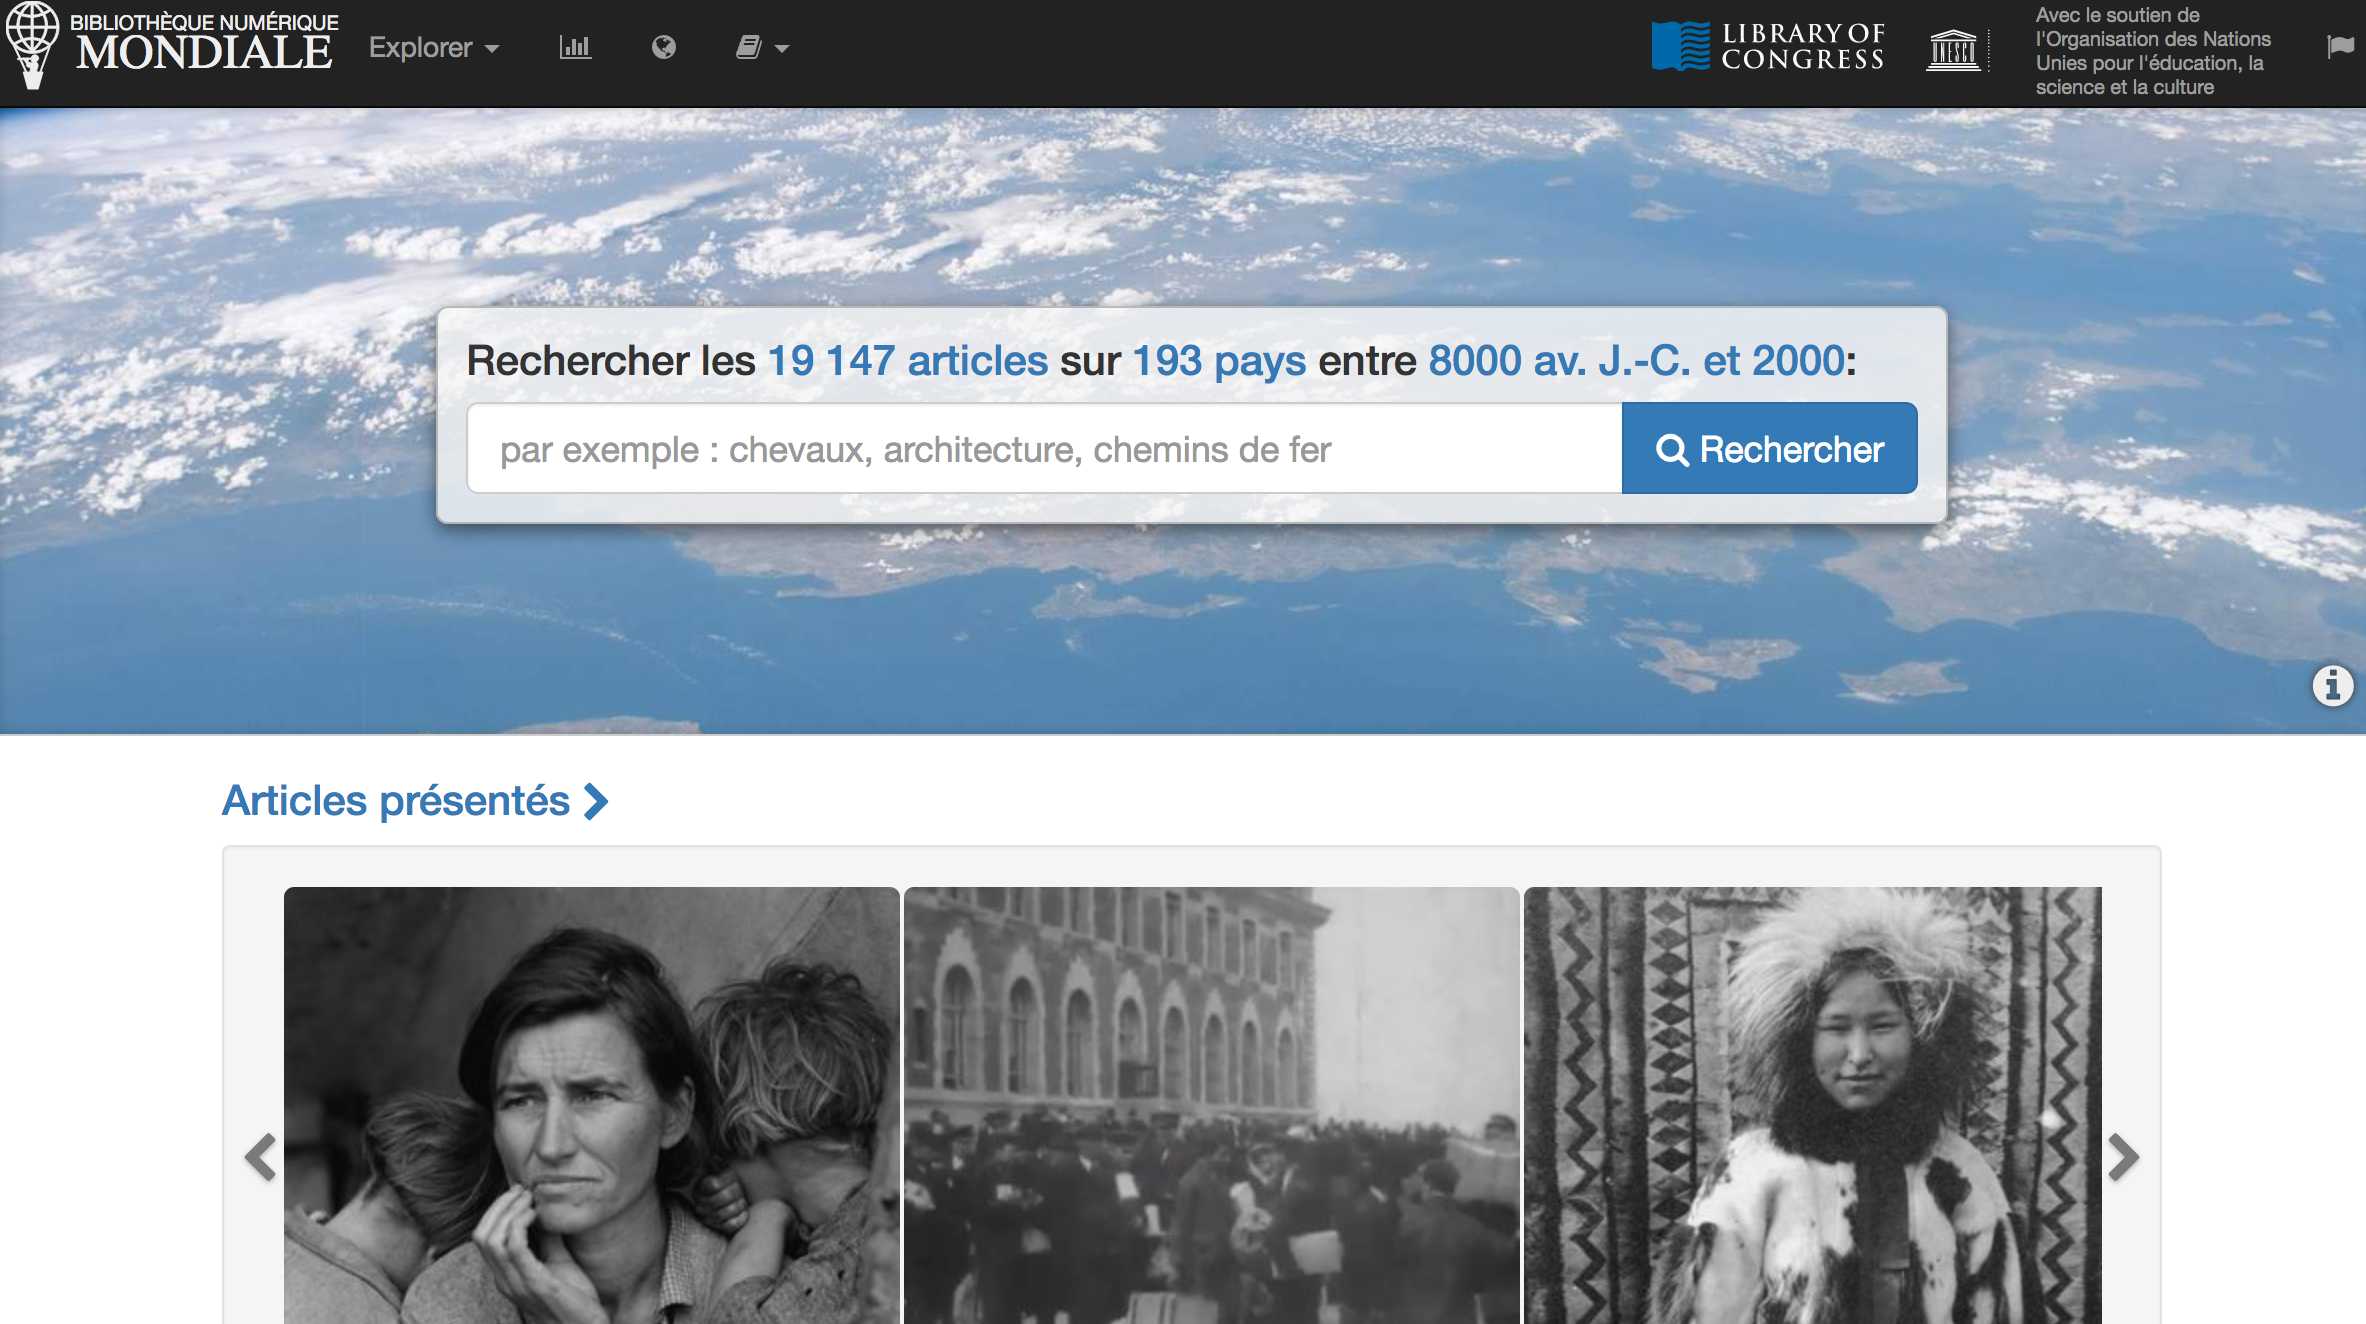
\includegraphics[width=15cm]{unesco}
\caption{Capture-d'écran de la plateforme du projet de Bibliothèque numérique mondiale.}
\end{figure}

La révolution numérique a fortement ébranlé l'\gls{ue} qui, par crainte de manquer ce tournant économique, énonce en 2010 diverses mesures dans son agenda Europe 2020, dont une spécifiquement consacrée à la numérisation du patrimoine culturel européen à travers Europeana\footnote{\cite{coutts_stepping_2017}}. Cet objectif, loin d'être nouveau, incarne l'évolution d'une volonté politique qui remonte à 2001. Retour sur l'histoire de ces principales actions politiques soutenant les entreprises de numérisation :

Les principes de Lund, définis en 2001, invitent les états membres à collaborer pour proposer un alignement de leurs programmes de numérisation, afin de favoriser la valorisation du patrimoine numérique et l'émergence d'une nouvelle forme d'économie\footnote{\cite{foulonneau_recherche_2003}}.

Consciente des nombreuses barrières technologiques à la mise en place d'une numérisation à l'échelle européenne et au développement d'un marché économique, l'\gls{ue} s'intéresse également à l'interopérabilité et publie en 2002 un rapport sur les bonnes pratiques, \textit{DigiCULT : paysages technologiques pour l'économie culturelle de demain, Faire connaître la valeur de l'héritage culturel}  \footcite{salzburg_research_forschungsgesellschaft_digicult_2002}\footcite{thylstrup_politics_2018}. 
 
Ces principes s'incarneront sous plusieurs formes : le programme MINERVA\footnote{MINERVA vise à mettre en place un réseau de soutien politique pour harmoniser les entreprises de numérisation visant à proposer notamment, des recommandations pour les métadonnées et l'interopérabilité des plateformes. \cite{claerr_manuel_2011}.} en 2003, \textit{The European Library}\footnote{Bibliothèque numérique servant de portail à différentes bibliothèques nationales et qui servira d'\gls{agr} de contenus pour la future Europeana, avant que le projet ne soit gelé en 2016.} en 2005 et Europeana en 2008\footnote{\cite{coutts_stepping_2017}}, et serviront de base pour définir le cadre politique et l'édition d'un certains nombres de recommandations\footnote{\cite{noauthor_commission_2011}}. Certains autres projets furent initiés par l'\gls{ue} durant ces mêmes années à l'instar de MICHAEL \textit{Multicultural Inventory of Cultural Heritage in Europe}, poursuivant des buts similaires et contribuant à rendre parfois trop touffu l'organigramme des initiatives\footnote{\cite{association_pour_le_patrimoine_naturel_et_culturel_du_canton_de_vaud_patrimoine_2012}}. Afin de clarifier les choses, l'\gls{ue} a choisi de concentrer ses forces dans la plateforme d'Europeana.

La Commission européenne publie en 2011 des \textit{COMMISSION RECOMMENDATION on the digitisation and online accessibility of cultural material and digital preservation}, qui précisent notamment que : 
\begin{itemize}
\item La numérisation du patrimoine culturel européen comprend les objets imprimés, les photographies, collections des musées, documents d'archives, sons, documents audiovisuels, monuments et sites archéologiques.
\item Pour couvrir les coûts élevés de la numérisation, des partenariats public-privé doivent être mis en place.
\item Numériser est une manne économique, puisque ces données permettront aux industries créatives et culturelles de proposer de nouvelles formes de services et les aideront dans cette phase de transition liée à la révolution numérique. Il est urgent d'agir sous peine de manquer cette transformation numérique des industries : \inquote{\textit{If Member States do not step up their investments in this area, there is a risk that the cultural and economic benefits of the digital shift will materialise in other continents and not in Europe}.\footnote{\cite{noauthor_commission_2011}}} 
\item Pour diminuer les coûts, il est important d'améliorer les infrastructures techniques existantes et de collaborer à l'échelle européenne pour la mise en place des meilleures solutions.
\item Certaines législations doivent être adaptées pour répondre aux besoins d'échanges et d'interopérabilité de ces initiatives. Lever ces barrières doit être fait sur le plan national et européen pour garantir un degré d'uniformisation. 
\item La conservation des données numérisées doit être faite sur le long-terme.
\item Mettre en place des bases de données favorisant l'identification des \oe{}uvres sous droit d'auteur et faciliter leurs numérisations.
\end{itemize}
Ces recommandations spécifient également que le projet Europeana doit parvenir à numériser 30 millions d'objets d'ici 2015, afin de parvenir à la numérisation de l'intégralité de l'héritage culturel d'ici à 2025\footnote{\cite{coutts_stepping_2017}}.

Faisant suite aux recommandations de la Commission, la directive sur certains usages des \oe{}uvres dites orphelines, datée d'octobre 2012\footnote{Les \oe{}uvres orphelines sont des \oe{}uvres protégées par le droit d'auteur, mais dont le détenteur des droits ne peut être identifié.}, vise à permettre la numérisation des \oe{}uvres sous droit, si certains conditions sont remplies. Une fois qu'une recherche sérieuse des détenteurs des droits a été menée, une base de donnée permet de les enregistrer avant de procéder à leurs numérisations\footnote{\cite{noauthor_orphan_nodate}} .

En 2015, l'\gls{ue}, consciente que la révolution numérique a rétabli des barrières que les politiques européennes s'étaient efforcées de réduire dans le monde physique, notamment concernant la libre circulation des données, inhérente à la réussite de tout projet de numérisation de masse, propose la mise en place d'un marché unique numérique\footnote{\cite{hoekstra_proposed_2019}}. L'idée est de pouvoir ainsi concurrencer les leaders mondiaux qui bénéficient eux-mêmes de vastes marchés économiques\footnote{\cite[p.3]{viola_vers_2017}} en se dotant des moyens pour moderniser et décloisonner cette présence numérique\footnote{\cite{viola_vers_2017}}. Pour pouvoir proposer un meilleur accès, sans frontières, aux commerces en ligne, il faut notamment lever le principe de géolocalisation et moderniser les lois sur le droit d'auteur\footnote{\cite{noauthor_eu_2015}}. Le marché unique numérique est pensé pour aider l'\gls{ue} à rattraper son retard économique.

\begin{quotation}
[\textit{Traduction}]
L'\gls{ue} est très en retard par rapport à d'autres pays et régions concernant les échanges commerciaux en ligne, les compétences numériques, la mise en place de règlements appropriés et l'investissement dans les infrastructures numériques. Cela est unanimement reconnu comme une conséquence d'un marché unique très fragmenté qui entrave les échanges commerciaux numériques entre pays européens et gêne le développement de jeunes plateformes européennes et start-ups.
\footnote{\inquote{\textit{The EU is still lagging far behind other countries and regions when it comes to digital cross-border trade, digital skills, innovative regulation and investment in digital infrastructure. It is widely acknowledge that this is to a large extent the result of a fragmented Single Market, which hinders digital trade between EU-countries and hampers the scaling of young European digital platforms and start-ups}}\cite{dittrich_balancing_2017}.}
\end{quotation}

Les résultats de la mise en place de ce marché tardent à se faire sentir et certains auteurs argumentent que plutôt que de libéraliser, les propositions sont venues ajouter une couche de régulation administrative supplémentaire aux initiatives numériques\footnote{\cite{noauthor_next_nodate}}. Certains s'accordent à dire que l'\gls{ue} s'est trompée de combat et plutôt que d'accroître la compétitivité par ce marché unique numérique, elle devrait s'attaquer aux véritables barrières qui se trouvent dans les lois sur le droit d'auteur, trop souvent envisagées uniquement du point de vue des créateurs de l'\oe{}uvre, voir plutôt de celui des détenteurs des licences\footnote{\cite{schroff_politics_2018}}.

Le nouvel agenda pour la culture, publié en mai 2018, est construit sur l'idée du marché numérique unique, et s'engage à mettre en place un réseau de centres de compétence à travers l'\gls{ue} afin de préserver le patrimoine bâti par le biais de la numérisation de masse, et renforcer la collaboration entre acteurs culturels, industries créatives, autorités locales, partenaires sociaux, instituts de recherche et d'éducation, autour des initiatives de numérisation\footnote{\cite{drennan_european_2018}}. 

L'\gls{ue} s'intéresse de près à l'évolution de ces entreprises de numérisation. La Commission européenne a publié en 2018 un rapport sur cette progression, \textit{European Commission report on Cultural Heritage: Digitisation, Online Accessibility and Digital Preservation}\footnote{\cite{noauthor_european_2019}}. Avec pour objectif d'évaluer les progrès réalisés concernant l'application des recommandations de 2011, il propose un état des lieux des entreprises de numérisation au sein des pays membres et établit certaines bonnes pratiques\footnote{\cite{noauthor_council_nodate}}. Parmi les faits à relever :  un tiers des états font usage de la numérisation et de la 3D pour la préservation du patrimoine, bien qu'il y ait encore un manque de connaissances pratiques constaté dans les milieux professionnels ; un accroissement des partenariats public-privé est observé, pour mieux faire face aux coûts élevés de ces entreprises ; il est complexe d'identifier les \oe{}uvres étant du domaine public ; les \oe{}uvres sous droit d'auteur sont très peu représentées au sein des collections et la directive concernant les \oe{}uvres orphelines est peu utilisée car trop chère à déployer\footnote{\cite{noauthor_european_2019}}\footnote{\cite{zeinstra_research:_2016}}.

Signée durant les \textit{Digital Days 2019}, une nouvelle déclaration européenne \textit{the Declaration of cooperation on advancing digitisation of cultural heritage} s'engage à favoriser la coopération pour faire avancer les entreprises de numérisation patrimoniale. Elle s'articule autour de trois axes\footnote{\cite{noauthor_eu_2019}}.
\begin{enumerate}
\item La mise en place d'une initiative européenne pour avancer la numérisation 3D des monuments, sites et artefacts culturels et patrimoniaux.
\item L'usage de ces ressources numériques pour développer l'engagement citoyen et favoriser l'émergence d'entreprises innovantes dans tous les secteurs.
\item Encourager les initiatives entre partenaires de secteurs et pays différents pour augmenter la capacité de développement de cette numérisation de masse de l'héritage culturel.
\end{enumerate}
Il est intéressant de spécifier que le projet Time Machine est cité par la déclaration comme projet répondant à ces objectifs.

Consciente que les enjeux sont du côté de la gestion des droits des \oe{}uvres numériques, l'\gls{ue} a adopté la \textit{Directive on open data and the re-use of public sector information} en avril 2019. Cette dernière spécifie que les \oe{}uvres libres de droit numérisées doivent demeurer libres de droit. Si un droit exclusif pour numériser ou reproduire une \oe{}uvre est imposé, il ne doit pas excéder une période de dix ans et être au maximum non contraignant. \inquote{\textit{Any licences for the re-use of public sector information should in any event place as few restrictions on re-use as possible, for example limiting them to an indication of source.}}

L'accélération du rythme de publication des recommandations et des directives, semble indiquer que l'\gls{ue} a de hautes attentes, concernant la numérisation de son patrimoine. L'incendie récent survenu à Notre-Dame de Paris est venu encore renforcer un débat déjà existant\footnote{\cite{noauthor_european_2019}}. Europeana ayant dépassé ses objectifs de quantité, l'\gls{ue} semble désormais choisir la voie du développement de la qualité (multilinguisme, plateforme, amélioration de la médiation du contenu etc.)\footnote{\cite{noauthor_european_2019}}.

\begin{figure}[H]% force à placer l'image au sein de notre balise figure
%\centering
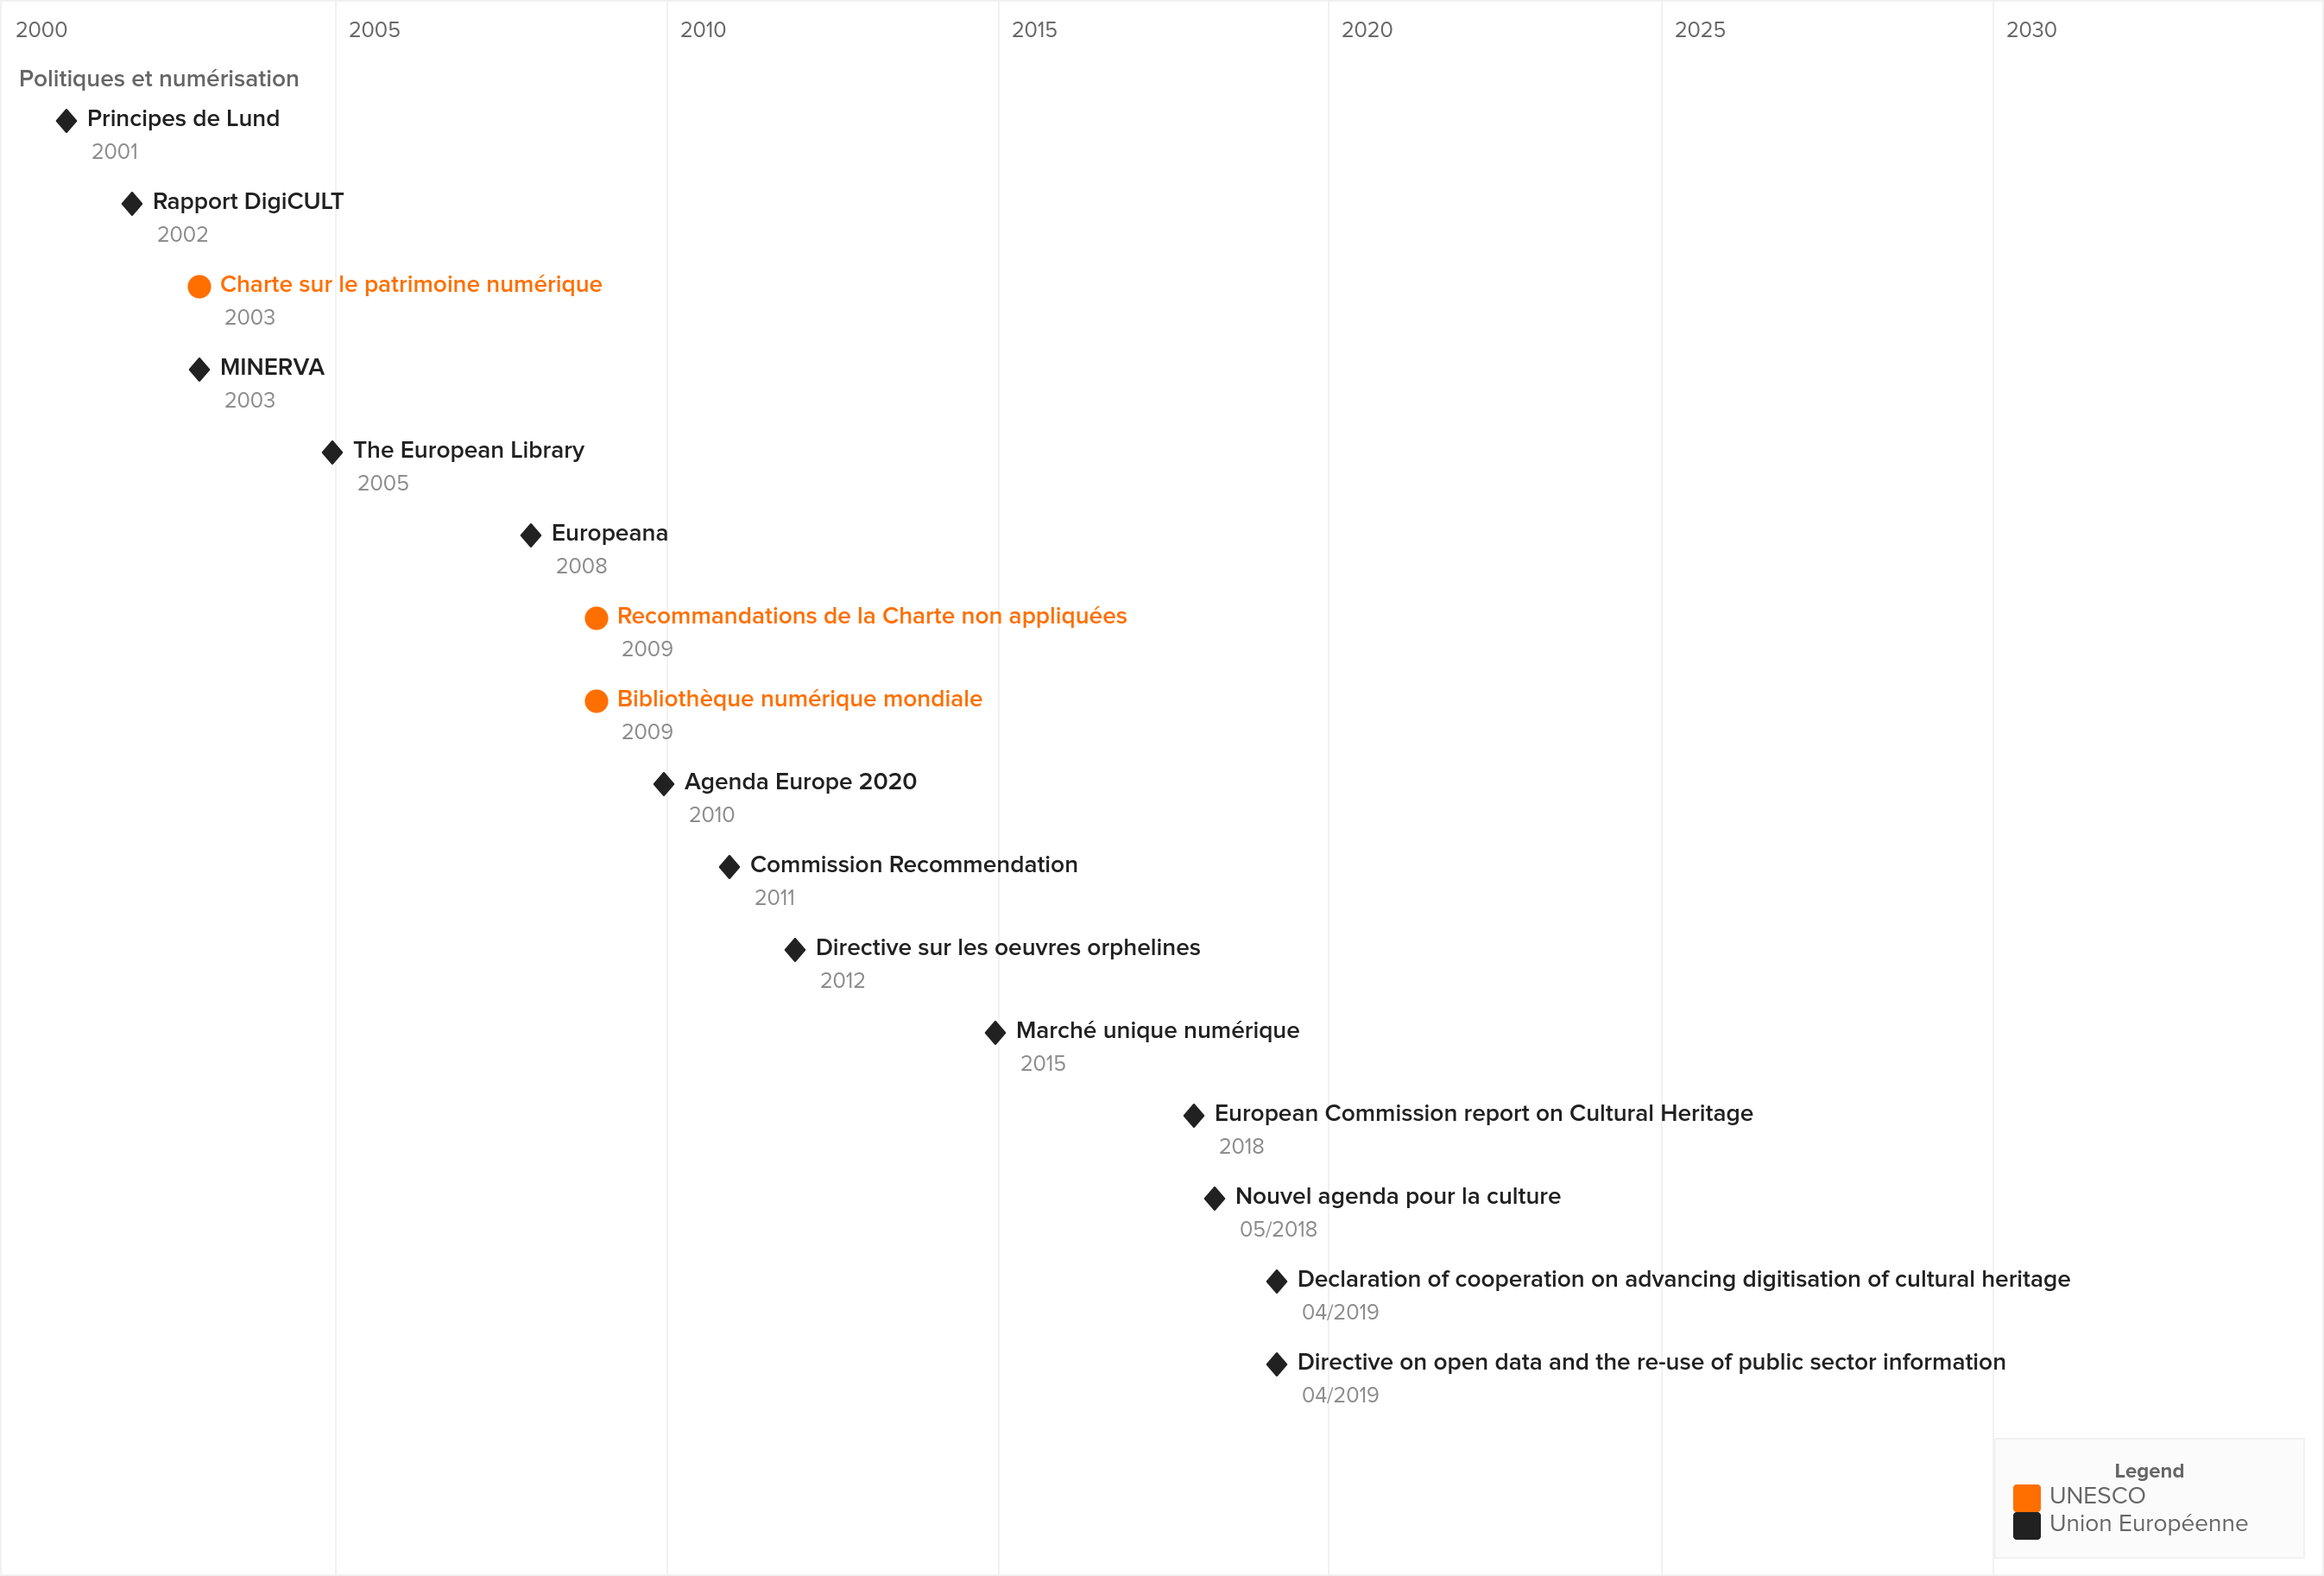
\includegraphics[angle=90, scale=0.27]{politiques_numerisation.png}
\caption{Frise temporelle, \textit{Politiques et numérisation}.}
\end{figure}
\newpage

%========TABLEAU LEçONS
\section{Leçons d'histoire pour Time Machine}

De cette revue du contexte historique, nous avons déduit certaines \inquote{leçons}. %éléments appelés à impacter le futur projet Time Machine. %Nous vous proposons à la page suivante un tableau résumant ces \inquote{leçons de l'histoire}.

\begin{table}[H]
\centering
%

\begin{tabular}{|l|l|lll}
\cline{1-2}
\cellcolor[HTML]{2E1A46}{\color[HTML]{FFFFFF} \textbf{\begin{tabular}[c]{@{}l@{}}Contexte \\ historique\end{tabular}}}    & \cellcolor[HTML]{2E1A46}{\color[HTML]{FFFFFF} \textbf{Points d'attention pour Time Machine}}                                                                                                                                                               &  &  &  \\ \cline{1-2}
{\color[HTML]{2E1A46} }                                                                                                   & Le projet de bibliothèque universelle n'est pas nouveau.                                                                                                                                                                                                   &  &  &  \\ \cline{2-2}
{\color[HTML]{2E1A46} }                                                                                                   & \begin{tabular}[c]{@{}l@{}}Les développements technologiques impactent la portée et le cadre \\ des projets.\end{tabular}                                                                                                                                  &  &  &  \\ \cline{2-2}
\multirow{-3}{*}{{\color[HTML]{2E1A46} \textbf{\begin{tabular}[c]{@{}l@{}}Prémisses \\de la \\numérisation\end{tabular}}}} & \begin{tabular}[c]{@{}l@{}}La version numérique n'est pas parfaitement identique à la version\\ physique du document.\end{tabular}                                                                                                                         &  &  &  \\ \cline{1-2}
{\color[HTML]{2E1A46} }                                                                                                   & Pas de définition figée pour les projets de numérisation de masse.                                                                                                                                                                                         &  &  &  \\ \cline{2-2}
{\color[HTML]{2E1A46} }                                                                                                   & \begin{tabular}[c]{@{}l@{}}Les collections numériques ne sont pas le reflet de la connaissance \\ universelle et portent des biais hérités des collections physiques et\\ motivés par leurs sources de financement.\end{tabular}                           &  &  &  \\ \cline{2-2}
{\color[HTML]{2E1A46} }                                                                                                   & \begin{tabular}[c]{@{}l@{}}Différents acteurs impliquent différents intérêts qui se mêlent au sein \\ d'un projet. Point de vue technologique, point de vue patrimonial, \\ point de vue du public ; partenaires publics, partenaires privés.\end{tabular} &  &  &  \\ \cline{2-2}
{\color[HTML]{2E1A46} }                                                                                                   & \begin{tabular}[c]{@{}l@{}}La construction d'une collection numérique peut être définie par des \\ choix politiques.\end{tabular}                                                                                                                          &  &  &  \\ \cline{2-2}
{\color[HTML]{2E1A46} }                                                                                                   & \begin{tabular}[c]{@{}l@{}}La taille du projet induit un besoin de standardisation et la mise en \\ place de bonnes pratiques.\end{tabular}                                                                                                               &  &  &  \\ \cline{2-2}
{\color[HTML]{2E1A46} }                                                                                                   & \begin{tabular}[c]{@{}l@{}}Ouverture et protection du droit d'auteur ne sont pas synonymes, et \\ les enjeux légaux réels.\end{tabular}                                                                                                                    &  &  &  \\ \cline{2-2}
\multirow{-7}{*}{{\color[HTML]{2E1A46} \textbf{\begin{tabular}[c]{@{}l@{}}Passage à \\ l'échelle\end{tabular}}}}          & \begin{tabular}[c]{@{}l@{}}Le projet se construit pour être au service de l'utilisateur final et \\peut être influencé par ce dernier.\end{tabular}                                                                                                       &  &  &  \\ \cline{1-2}
{\color[HTML]{2E1A46} }                                                                                                   & La numérisation est au programme des politiques européennes.                                                                                                                                                                                               &  &  &  \\ \cline{2-2}
{\color[HTML]{2E1A46} }                                                                                                   & Il y a une volonté d'aligner les initiatives.                                                                                                                                                                                                  &  &  &  \\ \cline{2-2}
{\color[HTML]{2E1A46} }                                                                                                   & Des partenariats public-privé servent à financer les projets.                                                                                                                                                                                            &  &  &  \\ \cline{2-2}
{\color[HTML]{2E1A46} }                                                                                                   & \begin{tabular}[c]{@{}l@{}}Les données numérisées permettent l'émergence d'un nouveau secteur \\ économique.\end{tabular}                                                                                                                                  &  &  &  \\ \cline{2-2}
{\color[HTML]{2E1A46} }                                                                                                   & \begin{tabular}[c]{@{}l@{}}Les législations concernant le droit d'auteur doivent être adaptées et \\ uniformisées.\end{tabular}                                                                                                                            &  &  &  \\ \cline{2-2}
{\color[HTML]{2E1A46} }                                                                                                   & Les données numérisées doivent être conservées sur le long-terme.                                                                                                                                                                                          &  &  &  \\ \cline{2-2}
{\color[HTML]{2E1A46} }                                                                                                   & \begin{tabular}[c]{@{}l@{}}Renforcer la coopération autour des entreprises numériques est dans\\ l'agenda européen.\end{tabular}                                                                                                                           &  &  &  \\ \cline{2-2}
{\color[HTML]{2E1A46} }                                                                                                   & Numériser inclut le patrimoine bâti, avec l'aide  de la 3D.                                                                                                                                                                                                &  &  &  \\ \cline{2-2}
\multirow{-9}{*}{{\color[HTML]{2E1A46} \textbf{\begin{tabular}[c]{@{}l@{}}Politiques et \\ numérisation\end{tabular}}}}   & Les œuvre libres de droit doivent le demeurer, une fois numérisées.                                                                                                                                                                                        &  &  &  \\ \cline{1-2}
\end{tabular}
\centering
\caption{Leçons d'histoire pour Time Machine}
\end{table}

%====================CHAPITRE 2 keyword : enjeux

\chapter{\textit{Comment} numériser en masse}

L'histoire des projets de numérisation a permis de mettre en lumière la complexité et la diversité de ces entreprises, s'inscrivant à la fois dans une forme de rupture et de continuité avec ce qui a précédemment été. Si de nombreux scientifiques s'intéressent au \textit{comment} (quelles réponses apporter aux défis techniques, légaux etc. ?) des projets de cette envergure, peu osent s'attaquer au \textit{pourquoi} (quelles formes de connaissance sont créées par ces projets, quels sont les impacts sur l'organisation des entreprises culturelles, de quel contexte politique sont-ils issus, etc. ?)\footnote{\cite{thylstrup_politics_2018}}. Les projets ne se laissent pourtant pas facilement restreindre à des aspects opérationnels et techniques, alors même que ces derniers sont déjà très nombreux et impliquent la définition de nombreuses typologies de standards : 

\begin{quotation}
[\textit{Traduction}]
Ces projets de numérisation de masse partagent de nombreuses caractéristiques. Ils impliquent le développement de standards pour une numérisation uniforme et pour les métadonnées techniques et descriptives ; la prise de décisions sur les droits d'utilisation ; le choix des logiciels de stockage, de l'environnement de mise à disposition des ressources et du matériel informatique.
\footnote{\inquote{\textit{These mass digitization projects have many similar characteristics. They require standards for uniform digitization, standards for descriptive and technical metadata, decision on rights and permissions, decisions on software for storage and end-user access, and decisions on hardware and operating environments}}\cite[p.11]{kowalczyk_digital_2018}.}
\end{quotation}

Nanna Bonde Thylstrup ose voir au-delà du \textit{comment}, en argumentant que ce changement de contenant (passage d'informations cloisonnées dans un objet physique à la création de jeux de données) induit la création de nouvelles voies de transmission de la connaissance et la redéfinition des aspects politiques, légaux, financiers associés. Ce qui aboutit à d'inévitables controverses découlant de tant d'intérêts mélangés.

\begin{quotation}
[\textit{Traduction}]
Les méthodes de numérisation de masse, créent de nouvelles formes de connaissances et de nouveaux moyens de la découvrir. Ce qui à première vue semble se limiter à un simple acte de numérisation (la transformation des limites physiques d'un livre, en un jeu de données libre), révèle, si nous le regardons de plus près, un processus complexe, foisonnant de diverses controverses politiques, légales et culturelles.
\footnote{\inquote{\textit{The practice of mass digitization is forming new excuses of knowledge, and new ways of engaging with that knowledge. What at first glance appears to be a simple act of digitization (the transformation of singular books from boundary objects to open sets of data), reveals on closer examination, a complex process teeming with diverse political, legal, and cultural investments and controversies}}\cite[p.1]{thylstrup_politics_2018}}
\end{quotation}

Pour mieux analyser ces projets et oser s'intéresser au \textit{pourquoi} (dans la troisième partie de ce mémoire), il nous faut d'abord présenter leur matière même, ce \textit{comment}. Nous vous présentons dans ce chapitre leurs principales caractéristiques puis certains enjeux qui en découlent\footnote{Ces derniers étant très nombreux et de nouveaux ne cessant d'apparaître, nous ne serions prétendre à une absolue exhaustivité.}. Bien que les projets de numérisation de masse ne se laissent que mal résumer tant leurs complexités et spécificités sont grandes, notre revue de la littérature et notre expérience de stagiaire nous ont permis de définir les problématiques minimales induites par ces initiatives. 

%======= CARACTERISTIQUES DES PROJETS DE NUMERISATION
\section{Caractéristiques des projets}\label{caracteristique}

Avant de tenter une caractérisation des projets de numérisation de masse, rappelons brièvement la signification du terme numérisation. Dans le monde du patrimoine, la numérisation implique traditionnellement\footnote{\cite[p.37]{dufrene_numerisation_2013}} : 

\begin{itemize}
\item La conversion d'un objet physique ou analogique (en général des images, fichiers audio ou vidéo ou du texte) en une suite de données interprétables par des machines.
\item La conversion des catalogues sur fiche des bibliothèques selon le même processus.
\end{itemize}

Le projet Time Machine y ajoute une troisième dimension puisqu'il désigne également : 
\begin{itemize}
\item La transformation du patrimoine bâti ou phénomène géographique en modèles 3D.
\end{itemize}

Dans le cadre de ce mémoire, la définition de la numérisation se veut la plus large possible et peut se résumer par la création d'un contenu, copie ou enregistrement numérique, d'une information analogique contenue par un document, artefact, son, performance, élément géographique ou phénomène naturel.

Au-delà de l'acte lui-même, numériser désigne une série de processus d'analyse intellectuelle et d'indexation visant à satisfaire les besoins des utilisateurs avec, pour double objectif, d'assurer la préservation du document au-delà de la durée de vie de son support et de pouvoir valoriser le document numérisé et son modèle original.\footnote{\cite{noauthor_numerisation_2013}}. Tout projet de numérisation pose une série de difficultés, liées aux coûts souvent élevés, au temps nécessaire pour la réalisation, à la qualité de l'indexation, à la conservation à long-terme des données, au coût induit par la maintenance des équipements informatiques et à la qualification des équipes chargées de gérer la masse des documents numérisés\footnote{\cite[p.37]{dufrene_numerisation_2013}}. 

Les objets choisis pour la numérisation ne sont pas systématiquement le fait de politiques de sélection mais découlent des ressources financières, du temps, de la qualité et des objectifs que l'on veut accomplir : \inquote{\textit{Therefore, looking to our traditional media, digitization is not a question of selection according to certain criteria, but according to financial resources, time line, priorities, quality and/or aims we want to reach.\footnote{\cite[p.19]{association_pour_le_patrimoine_naturel_et_culturel_du_canton_de_vaud_patrimoine_2012}}}}

Karen Coyle définit les projets de numérisation de masse comme la conversion de matériel à une échelle industrielle, sans véritable politique de sélection et utilisant les techniques de \gls{reo} pour permettre les recherches plein-texte : \inquote{\textit{ [...] mass digitization refers to converting materials on an industrial scale without curating specific materials for digitization. OCR is used to make the full text of digitized documents searchable}}\footnote{\cite{coyle_mass_2006}}. 

Iris Xie met en avant leurs plateformes d'accès, en les désignant comme les nouvelles générations de systèmes de découverte, offrant un accès centralisé vers une grande variété du patrimoine culturel et scientifique et caractérisés par plusieurs millions de titres, des formats divers, une politique de gestion du droit d'auteur, une politique de sélection, et des degrés d'accessibilité dérivés en fonction, ainsi que par la mise en place de standards techniques pour assurer l'interopérabilité\footnote{\cite[p.23]{xie_discover_2016}}.

Comme déjà mentionné\footnote{Pour plus de détails, référez-vous à la section \ref{echelle}.}, certains auteurs présentent\footnote{\cite{jones_public_2017}} ou osent une distinction entre les projets menés par des partenaires commerciaux et les projets issus des institutions publiques. Justifié par un enjeu plus grand mis sur l'accessibilité des données dans le premier cas, et par la prise en compte de modération humaine dans la gestion des collections, avec un accent plus développé sur les aspects liés à la préservation des données et la réutilisations des métadonnées existantes dans le deuxième cas. Les objectifs de création d'un moteur de recherche universel et le développement de nouveaux services basés sur l'indexation plein-texte d'immenses corpus de données aux formats divers et issus du domaine public restent communs aux deux types d'initiatives\footnote{\cite[p.47]{lampert_ramping_2018}}. 

Il est toutefois certain que la complexité de tels projets ne saurait faire l'objet d'une seule définition tant les intérêts qu'ils mêlent soulèvent de multiples questions, \inquote{\textit{Mass digitization brings together so many disparate interests and elements that any monotheoretical lens would fail to account for the numerous political issues arising within the framework of mass digitization\footnote{\cite[p.5]{thylstrup_politics_2018}}}}. 

La numérisation de masse semble surtout se distinguer des autres formes de numérisation par une contrainte moins importante sur la sélection des sources et par la vitesse des processus liée aux développements technologiques et à l'automatisation. Ces entreprises ne sont dès lors pas résumables en un tout ou par l'une de leurs parties, elles sont constituées de différents assemblages\footnote{\cite[p.26]{thylstrup_politics_2018}}. Si les projets sont difficiles à catégoriser, ils se regroupent derrière la mission de permettre un meilleur accès aux collections des institutions patrimoniales\footnote{\cite[p.58]{lampert_ramping_2018}}.

Avec l'avènement et la construction de notre société numérique, le développement d'une économie liée et l'arrivée de nouvelles générations, il y a désormais un sentiment d'urgence à numériser le savoir qui motive la poursuite de projets de grande ampleur. Celui-ci fait écho aux premières craintes des informaticiens qui prédisaient que les pratiques des utilisateurs seraient à l'avenir uniquement orientées en ligne.

\begin{quotation}
[\textit{Traduction}]
Dans un contexte d'accroissement de la dominance numérique et puisque la plupart des biens patrimoniaux et culturels existent incontestablement uniquement sous une forme physique, la numérisation demeure comme par le passé, un élément clé de tous futurs développements.
\footnote{\inquote{\textit{In the light of increasing digital dominance, however, and the incontrovertible fact that so much of the world's knowledge and cultural outputs still exist only in physical form, digitisation is as much a key element in future digital developments as it has been in the past}}\cite[p.4]{coutts_stepping_2017}}
\end{quotation}

\begin{quotation}
[\textit{Traduction}]
Il existe aujourd'hui des risques considérables à ne pas faire progresser les projets de numérisation. Les nombreux utilisateurs exclusivement numériques pourraient ignorer, voire ne jamais être informés de l'existence de contenus pertinents pour leurs besoins et intérêts. Une connaissance négligée à travers le temps, devient une connaissance perdue, au détriment de tous.
\footnote{\inquote{\textit{There are considerable risks in not advancing digitisation at this time. The numerous digital-only users may ignore or never know of key content which is relevant to their interests and needs. Neglected knowledge, over time, becomes lost knowledge, to the detriment of all}}.\cite[p.4]{coutts_stepping_2017}.}
\end{quotation}

Cette intensification des projets commence à ouvrir les débats autour des questions du \textit{pourquoi} de la numérisation, et certains auteurs s'attachent à proposer de nouveaux angles d'analyse, interrogeant la typologie des acteurs de la numérisation et les leçons à apprendre de ces initiatives\footcite[p.47]{lampert_ramping_2018}\footnote{\cite{thylstrup_politics_2018}}.

%======= ENJEUX DES PROJETS DE NUMERISATION
\section{Enjeux des projets}
Nous avons choisi de présenter les enjeux qui nous ont semblés incontournables pour toute entreprise de numérisation, cependant le développement rapide de ces initiatives et des technologies numériques, nous interdit de prétendre être exhaustive. Ces derniers se construisent autour des questions liées à la mise en place d'une collaboration effective entre différents partenaires, au coût, au droit d'auteur, à l'interopérabilité découlant de choix techniques ou de la construction des corpus, ainsi qu'à la préservation et au stockage de ces données. Ces différents axes interagissent les uns avec les autres au sein d'un même projet, et les décisions relatives peuvent influencer sa réussite finale. 
L'arrivée de \textit{Google Books} a fortement impacté les stratégies des projets de numérisation et semble être l'origine de la nouvelle complexité de ces enjeux\footcite{dufrene_numerisation_2013}.

Les réponses apportées par certaines initiatives et par Time Machine à ces enjeux du \textit{comment} seront examinées respectivement dans la deuxième et la troisième partie du mémoire.
%===COLLABORATION
\subsection{Amener différents acteurs à collaborer }
Les projets de numérisation de masse ont poussé les bibliothèques à sortir de leur isolement. Pour arriver à une meilleure efficacité et une meilleure \inquote{compétitivité}, il a fallu travailler à inscrire la numérisation du patrimoine dans les objectifs de politique publique, définir plus précisément la notion d'Europe culturelle déjà existante dans l'agenda européen\footnote{Pour plus de détail référez-vous à la section \ref{politique}.}, agrandir l'offre à d'autres objets que les livres et partager les infrastructures existantes. Ce qui a conduit les \gls{glam}s à vouloir davantage coopérer au sein d'un même projet\footcite{dufrene_numerisation_2013}. 

\begin{quotation}
[\textit{Traduction}]
Les bibliothèques et archives sont très conscientes des opportunités offertes par la collaboration en regard de ce qui pourrait être fait en travaillant seul. Nous constatons une grande volonté de leur part à développer de telles initiatives. Les bibliothèques publiques et les musées sont les premiers à viser l'amélioration de leurs services au public par le biais de la collaboration et de la mise en commun de collections et d'infrastructures.
\footnote{\inquote{\textit{There is also a strong emphasis on the opportunities to achieve more by working with others than can be achieved by working alone, and this is specified by the library and archives sectors in particular. The public libraries and museums are prominent among those targeting improved public services through collaboration, and in sharing collections and infrastructure}}\cite[p.23]{coutts_stepping_2017}.} 
\end{quotation}

S'inscrivant dans le contexte multilatéral et international de la mondialisation, les projets doivent  orchestrer le double retour du local et du national\footcite[p.175]{dufrene_numerisation_2013}.

La collaboration est également nécessaire pour définir les choix techniques inhérents à la mise en commun des collections de diverses institutions, que les frontières nationales soient dépassées ou non par le cadre du  projet\footcite{moatti_bibliotheque_2012}. 

L'accélération des processus induits par l'envergure du projet implique souvent l'externalisation à un prestataire de certains actes de numérisation et le transport des documents concernés. L'organisation du flux des documents entre l'institution détentrice et le prestataire doit être soigneusement planifiée\footcite{ministere_de_la_culture_et_de_la_communication_:_direction_des_archives_de_france_ecrire_nodate}.

De la qualité de la collaboration découlent la possibilité de coordonner différentes initiatives de numérisation et de proposer une vision globale. Cet aspect semble souvent faire défaut aux initiatives, alors même que la collaboration est susceptible d'impacter fortement tous les autres enjeux\footcite{coutts_stepping_2017}. Parvenir à faire collaborer un nombre croissants de partenaires induit la mise en place d'outils de gestion, la définition d'un cadre, et la prise en compte du multilinguisme, et représente de fait un investissement nécessaire pour la réussite du projet\footcite{eschenfelder_nine_2019}.

\begin{quotation}
[\textit{Traduction}]
Bien entendu, chaque organisation sera confrontée à ses propres limites, et certaines initiatives ne pourront être poursuivies faute d'une collaboration effective mise en place avec soin. Collaborer implique un environnement délicat et finement équilibré [...]. Collaborer signifie travailler avec un ensemble cohérent et complexe de partenaires régionaux, nationaux et internationaux.
\footnote{\inquote{\textit{Ultimately, however, there will be limits to every organisation's options, and there will be initiatives that cannot go forward because they lack the collaborative commitment that they require. Collaboration is a finely balanced and delicate environment [...]. Collaboration means working with a coherent and complex set of regional, national, and international partnerships}}\cite[p.26]{coutts_stepping_2017}.}
\end{quotation}

 %===FINANCEMENT
\subsection{Financement et partenariats public-privé}

Les coûts élevés de la numérisation de masse et les limitations posées par le système de numérisation à la demande\footcite{maurel_quel_2017}\footnote{En général, le premier utilisateur paie pour le processus, le fichier est ensuite publié si libre de droit, sur la plateforme de l'institution.}, ont poussé les initiatives à chercher des solutions du côté des partenaires privés (individus, banques, fondations, médias, industries du tourisme etc.)\footcite{lopatin_library_2006}\footcite{yeates_collaborative_2006}. En général, comme les coûts sont fortement imputés à l'infrastructure\footnote{De grands progrès ont toutefois été faits sur les couches technologiques, la montée des coûts serait due aux recherches pour les droits d'auteur. \cite{stobo_i_2018}.}, ce sont vers des entreprises spécialisées dans ces technologies (à l'instar de Google, Proquest, IBM, Kodak)\footcite{dufrene_numerisation_2013}, que se tournent les institutions culturelles et patrimoniales. On trouve toutefois des engagements avec des fondations telles que Wikimedia et le recours au financement participatif ou \textit{crowdfounding}\footcite{noauthor_european_2019}\footnote{Cette piste demeure ambiguë, car pose des problèmes de réutilisation commerciale des \oe{}uvre ainsi numérisées. \cite{maurel_quel_2017}.}. 

L'arrivée des ces partenariats privés a reçu un accueil au départ très mitigé par crainte d'un monopole et de la réappropriation des ouvrages libres de droit publiés sous licence\footnote{Voir aussi à ce propos dans la section \ref{politique} la récente directive de l'\gls{ue}, sur les ouvrages libres de droit.}\footcite{association_pour_le_patrimoine_naturel_et_culturel_du_canton_de_vaud_patrimoine_2012}. Ces partenariats financiers entre institutions publiques et prestataires privés posent également des problèmes liés à la réutilisation des données, puisque certains prestataires imposent des conditions d'exclusivité\footcite{dufrene_numerisation_2013}\footnote{Voir aussi à ce propos dans la section \ref{politique} la récente directive de l'\gls{ue}, visant à limiter la durée des périodes d'exclusivité.}. De récentes études montrent toutefois que l'exclusivité tend à ne plus porter directement sur l'utilisation des oeuvres numérisées mais se déplace vers la commercialisation de services\footcite{maurel_quel_2017}.

En dépit de la prolifération de ces partenariats, il manque un socle de règles communes visant à limiter les risques de monopole de certains acteurs privés et à fixer un cadre permettant d'harmoniser et légitimer ces pratiques\footcite{dufrene_numerisation_2013}, afin de trouver l'équilibre entre des financements gouvernementaux, locaux, privés et caritatifs\footcite{yeates_collaborative_2006}. La mise en place d'une politique active de numérisation dans chaque état pourrait également permettre de rééquilibrer la situation\footcite{maurel_quel_2017}\footnote{Les Pays-Bas ont par exemple mis en place une loterie nationale pour répondre aux besoins financiers des institutions culturelles.}.

Malgré la créativité déployée par les initiatives pour parvenir à couvrir leurs frais, un manque est constaté dans l'organisation des projets, qui ont tendance à négliger la perspective du long-terme. Les projets financés par des bourses locales, nationales ou européennes sont souvent les plus susceptibles de présenter un modèle financier lacunaire\footcite{lampert_ramping_2018}. Ceci conduit à une multiplicité de projets financés, mais plus accessibles car les contenus n'ont jamais été mis à jour et les plateformes datées\footcite{eschenfelder_nine_2019}. 

Très peu d'études s'attachent à analyser le rapport entre l'audience générée par les plateformes et leurs coûts de production, ce qui permettrait aux initiatives de justifier ou d'adapter leurs investissements\footcite{moatti_bibliotheque_2012}.
 %===DROIT D'AUTEUR
\subsection{Droit d'auteur}

Les projets de numérisation de masse suscitent une prise de conscience de l'urgence à ne pas limiter les collections aux ouvrages libres de droit\footcite{dufrene_numerisation_2013}. La question du droit d'auteur devient incontournable, les institutions ayant la responsabilité de déterminer si le droit d'auteur s'applique ou non aux \oe{}uvres qu'elles souhaitent numériser\footcite{lopatin_library_2006}. 

La problématique du droit d'auteur, dans tout projet de numérisation, intervient de différentes manières\footcite{dufrene_numerisation_2013} :
\begin{itemize}
\item Certaines \oe{}uvres sont libres de droits, car dans le domaine public.
\item Certaines \oe{}uvres sont couvertes par le droit d'auteur, mais dites orphelines\footnote{Pour rappel, les \oe{}uvres orphelines sont des \oe{}uvres soumises au droit d'auteur mais dont le détendeur est inconnu.}.
\item Certaines \oe{}uvres existent nativement sous forme numérique et sont couvertes par des licences numériques.
\end{itemize}

Les exceptions au droit d'auteur sont réglées par un certain nombre de régimes de droits nationaux et quelques directives européennes visant à faciliter leur gestion. Il n'existe pas, en Europe, de réel équivalent aux exceptions définies par le \textit{fair use}\footnote{Le \textit{fair use} autorise cinq exceptions au droit d'auteur : le droit à opérer une copie privée, le droit de citation, le droit au pastiche ou à la caricature, l'usage pour l'enseignement, l'usage pour la recherche.} états-unien, qui a notamment servi à justifier la pratique de \textit{Google Books}. L'\gls{ue} est toutefois consciente des enjeux liés au droit d'auteur et a mis en place un certain nombre de recommandations et de directives\footnote{Pour plus de détail, référez-vous à la section, \ref{politique}}.

La montée des coûts des entreprises de numérisation de masse se justifie de plus en plus par la recherche des auteurs des \oe{}uvres sous droit\footcite{stobo_i_2018}. En effet dans l'environnement numérique, les détenteurs des droits ont un contrôle presque absolu sur l'utilisation de l'\oe{}uvre originale\footcite{pavlovic_serpent_2011}. Les détenteurs de ces droits refusent souvent de libérer les \oe{}uvres et ont peu d'intérêt à réduire les coûts pour les initiatives de numérisation, car cela représente une perte financière\footcite{stobo_i_2018}. Les acteurs cherchent surtout à maintenir un équilibre économique, chèrement acquis par les industries créatives\footcite{stobo_i_2018}. \inquote{\textit{The commercial publishers representing the greatest copyright holders were the most reluctant to grant the permission, fearing loss of their profits\footcite[p.54]{george_testing_2005}.}}

Cette situation conduit à une sous-représentation des \oe{}uvres à partir du 20\up{e} siècle au profit des \oe{}uvres plus anciennes généralement libres de droit, phénomène connu sous le nom de \inquote{Trou noir} du 20\up{e} siècle\footcite{dufrene_numerisation_2013}, \textit{20th century black hole}\footcite{noauthor_european_2019} ou encore \textit{digital black hole}\footcite{association_pour_le_patrimoine_naturel_et_culturel_du_canton_de_vaud_patrimoine_2012}.

Dans le cas des \oe{}uvres dites orphelines, la directive européenne de 2012\footnote{Pour plus de détail, référez-vous à la section, \ref{politique}} permet aux institutions de les numériser, mais impose la poursuite de recherches diligentes et le respect de nombreuses règles (interdiction de les utiliser ensuite pour un usage commercial, etc.) avant le lancement des processus\footcite{stobo_i_2018}. Ce qui s'avère trop coûteux pour la plupart des projets\footcite{noauthor_european_2019}.

Pour les \oe{}uvres encore soumises au droit d'auteur, mais non trouvables dans le commerce, il n'existe aucune directive visant à faciliter la recherche des détenteurs de droit et à lever les coûts imposés par ces derniers\footcite{noauthor_european_2019}.

Il y a un grand besoin de rétablir l'équilibre entre la protection des droits d'auteur et du profit qu'il génère pour certains, et la protection des intérêts du grand public et de la société à utiliser ces \oe{}uvres\footcite{pavlovic_serpent_2011}. Le droit d'auteur doit être adapté aux nouveaux modes de production de la connaissance\footcite{dufrene_numerisation_2013}. 

\begin{quotation} 
[\textit{Traduction}]
Ces dernières années, le droit d'auteur semble avoir dérivé vers une protection des détenteurs du droit au détriment des bénéfices pour la société. Les délégués semblent incapables ou peu disposés à changer cet équilibre par de nouvelles législations. Puisque les règlements existants sont mal équipés pour faire face aux nouvelles technologiques, les riches détenteurs de droits ont prestement utilisé ces nouvelles technologies pour accroître la protection de leurs \oe{}uvres ou intimider les usagers. \footnote{\inquote{\textit{In recent years, the balance of copyright appears to have tipped more toward the rights of copyright owners over the benefits to society, with legislators unable or unwilling to change that balance through new legislation. Because existing statutory language is ill-equipped to handle new technologies, wealthy and powerful copyright holders have been quick to use technology to expand protection of their works or to intimidate users}}\cite[p.54]{xie_discover_2016}.}
\end{quotation}

Solution possible à cette situation paradoxale, le \gls{oa} et l'\gls{os} méritent d'être davantage développés. Les exceptions au droit d'auteur doivent également être davantage explorées par les projets de numérisation de masse dont les institutions craignent trop souvent les retombées légales, ce qui ajouterait la gestion des risques à la liste des enjeux identifiés\footcite[p.661]{stobo_i_2018}. \inquote{Cependant ni la capitulation devant le droit d'auteur ni la transgression provocatrice des règles fondamentales ne peuvent résoudre le problème à la longue\footcite{association_pour_le_patrimoine_naturel_et_culturel_du_canton_de_vaud_patrimoine_2012}.}

\begin{quotation}
[\textit{Traduction}]
Compte tenu des coûts trop élevés associés à la recherche des auteurs des \oe{}uvres orphelines dans le cas de collections de grandes tailles, et du manque d'alternatives législatives, nous proposons que les institutions culturelles et patrimoniales apprennent à vivre en acceptant une certaine forme d'incertitude. Elles doivent explorer les perspectives offertes par une gestion consciente des risques dans leurs stratégies de gestion et mettre à profit le large champ des exceptions prévues dans les législations sur le droit d'auteur.
\footnote{\inquote{\textit{Given the unmanageable transaction costs associated with these orphan works schemes when dealing with collections of any notable size, as well as the lack of other useful cognate legislative form, we argue that Cultural Heritage Institutions must learn to live with the uncertainty inherent in copyright law : that is, they must explore risk management strategies in more depth, and utilise the full scope of the exceptions already available within the copyright regime}}\cite[p.661]{stobo_i_2018}.}
\end{quotation}

 %===SORTIR DES SILOS
\subsection{Sortir des silos - la quête de l'interopérabilité}

Tout projet de numérisation de masse implique à un certain moment, en plus de la \gls{num}, la réunion de collections déjà numériques et la mise à disposition de l'ensemble de ces données à travers une plateforme commune en ligne\footcite{lampert_ramping_2018}. Rassembler ces différentes données, puis les rendre trouvables, est complexe. De trop nombreuses \gls{db} ont été déployées par les institutions, éparpillant les données à travers des systèmes différents et contribuant à les enfermer et les isoler les unes des autres, dans des \inquote{silos}\footcite{institut_national_dhistoire_de_lart_lundisnum_nodate}. 

L'interopérabilité est un argument pour beaucoup, pour l'\gls{ue} qui souhaite mettre en place des procédures communes favorisant l'économie de la connaissance, pour les professionnels des bibliothèques et archives souhaitant sortir de leurs logiques de \inquote{silos} et pour le mouvement de \textit{\gls{os}}. L'objectif de l'interopérabilité est de faciliter les échanges de données entre les différents systèmes des institutions culturelles et patrimoniales\footcite{lopatin_library_2006} et de proposer des services permettant d'accroître les interactions avec ces ressources au sein d'un même réseau\footcite{xie_discover_2016}.

\begin{quotation}
[...] l'interopérabilité est devenue un enjeu à un autre niveau que par le passé. Il ne s'agit plus seulement d'échanger des notices pour éviter la redondance dans l'effort de catalogage, mais de mutualiser les outils à travers des \inquote{portails} pour tenter d'accrocher un usager devenu insaisissable\footcite[p.21]{bermes_web_2013}.
\end{quotation}

Alors que les standards et les bonnes pratiques apportent de nouvelles réponses aux enjeux techniques posés par la numérisation, ces derniers ne semblent pas encore avoir trouvé leur forme finale. 

De plus, un autre écueil contribue à isoler les collections des institutions culturelles et patrimoniales : celui de la sélection du contenu intellectuel. Un manque de coordination et de vision globale sur la création de ces collections les rend fortement disparates et complique davantage leur réunification au sein d'une même plateforme\footcite{coutts_stepping_2017}, augmentant également la redondance des données numérisées\footcite{institut_national_dhistoire_de_lart_lundisnum_nodate}. 

De l'attention apportée aux enjeux  techniques et aux enjeux sur le contenu, découle d'une part la qualité et la richesse de l'expérience proposée ensuite pour utilisateur, et d'autre part la qualité de la conservation sur le long-terme\footcite{xie_discover_2016}. 

Nous n'avons pas pour objectif de définir quelle sont les meilleurs pratiques à adopter, puisque ces dernières sont propres au contexte de chaque projet et liées aux objectifs utilisateurs, mais nous vous proposons une introduction des différents éléments auxquels toute initiative sera amenée à se confronter.

Il n'existe pas encore de modèle de donnée européen ou universel propre à assurer l'interopérabilité. La coopération entre institutions culturelles, professionnels de l'information et utilisateurs est essentielle pour la définition et l'implémentation d'un tel modèle\footcite{rasmussen_pennington_connecting_2019} qui devra être à la foi souple, cohérent et garant de la provenance des données\footcite{institut_national_dhistoire_de_lart_lundisnum_nodate}. Une étude européenne datée de 2004 définit trois critères à la réussite de l'interopérabilité : organisationnel, technique et sémantique\footcite[p.565]{zharova_influence_2015}. 
%\addcontentsline{toc}{subsubsection}{Enjeux techniques}
\subsubsection{Enjeux techniques}

%=== NUMERISATION
Les enjeux techniques se découpent en deux grandes familles. La première est liée aux processus de \gls{num}, ses choix portent sur la qualité des productions numériques et les formats\footnote{Le format désigne la nature d'un document informatique et permet d'identifier le logiciel nécessaire à sa lecture. Chaque fichier porte une extension en trois lettres indiquant le format (par ex. pdf pour les documents)} des fichiers ensuite produits. De cette qualité dépendent surtout la découverte proposée aux utilisateurs\footnote{Par exemple, une image sera accessible en plus ou moins haute résolution, ce qui ralentira ou non le navigateur de l'usager} et la préservation sur le long-terme des données\footnote{Pour plus de détails, référez-vous à la section \ref{preservation}}. Les bonnes pratiques privilégient le choix de formats ouverts (par exemple .tiff ou .png pour les images)\footnote{Un format ouvert par opposition aux formats propriétaires est un un fichier dont le code est accessible et transparent et peut être lu par différents logiciels.}. 

Pour s'assurer de la conformité aux critères de qualité, un contrôle doit être mis en place, faisant partie intégrante du projet. Il ne peut se réduire à une simple étape du processus.\inquote{Suivant les moyens disponibles et le niveau de qualité souhaité, on procédera au contrôle à différents moments de la production}\footcite[p.271]{claerr_manuel_2011}.

Si la recherche de la qualité des produits de la \gls{num} a motivé les premières initiatives, il semble que les projets de numérisation de masse ont appelé à une redéfinition des priorités pour produire plus en allégeant les processus, ce qui ne se fait pas sans difficulté. \inquote{Ansi la non-qualité et la sur-qualité sont des extrêmes à éviter}\footcite[p.271]{claerr_manuel_2011}. La qualité minimale se fixant sur l'usage et non sur les conditions de préservation. Les entreprises de numérisation de masse sont ainsi appelées à faire preuve de flexibilité, en appliquant des critères de qualité différents en fonction des documents\footcite{xie_discover_2016}. 

\newpage
\begin{figure}[H]% force à placer l'image au sein de notre balise figure
\centering
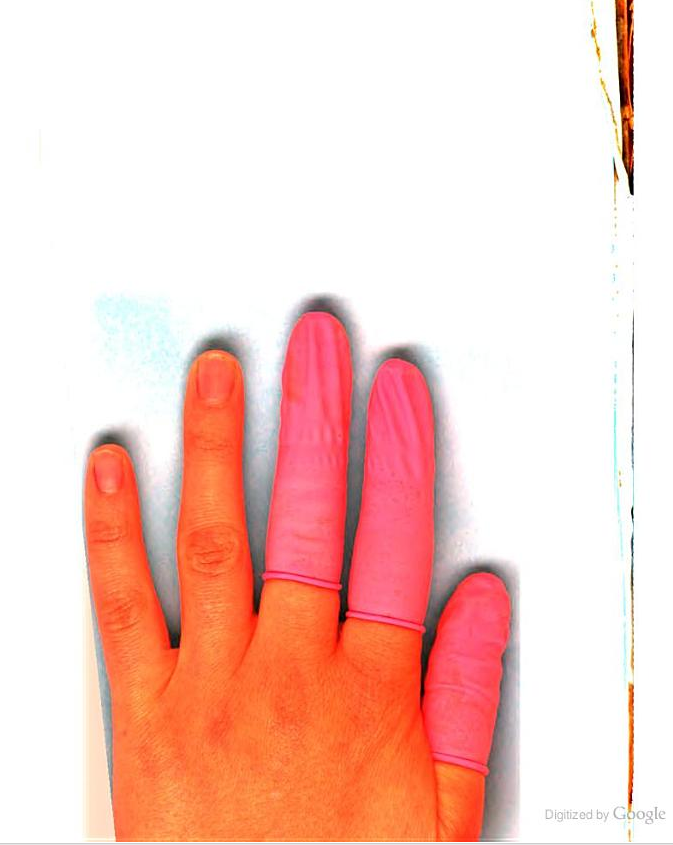
\includegraphics[scale=0.4]{qualite}
\caption{Image de mauvaise qualité, numérisée par Google ©\textit{Google Books}}
\end{figure}


%===METADONNEES

La deuxième famille des enjeux techniques est liée aux données servant à décrire les produits numérisés, soit les métadonnées. La quête de l'interopérabilité permettant de faire communiquer ces corpus de métadonnées décrivant les collections, indépendamment de l'environnement technique de leurs bases de données, est l'une des solutions pour la sortie des silos, ou c'est, en tous les cas, la présomption qui en est faite.

\inquote{\textit{It's a metadata's world, and you're just living in it\footcite[p.4]{pomerantz_metadata_2015}.}} Les métadonnées sont pleinement intégrées dans notre société et passent inaperçues. Nous n'avons pas toujours conscience que lorsque nous achetons un livre en librairie, c'est le titre, l'auteur ou la couverture qui auront motivés notre choix. Les informations servant à décrire le livre ont toujours été utilisées dans les bibliothèques, pour permettre de retrouver et classer les documents et sont à la base des catalogues. Les métadonnées nous servent à simplifier la réalité. Par exemple, \inquote{Camille} est mon prénom, mais ce n'est pas moi en tant que telle. 

Il existe plusieurs catégories de métadonnées, aux frontières parfois un peu floues : les métadonnées descriptives\footnote{Servant à simplifier l'objet ou l'information par le biais de mots-clés.}, les métadonnées administratives\footnote{Informations sur l'origine d'un document, par exemple une photographie numérisée avec tel scanner, telle résolution, sous telle licence}, les métadonnées structurelles\footnote{Informations sur l'organisation de l'objet, par exemple un livre se compose de chapitres.}, les métadonnées de préservation\footnote{Informations spécifiques à la préservation sur le long-terme.}, les métadonnées d'usage\footnote{Informations sur l'usage de l'objet, par exemple combien de fois un livre a-t-il été lu.}\footcite{pomerantz_metadata_2015}. Si les métadonnées descriptives ont été développées avec pour objectif d'améliorer la recherche sur internet, elles n'ont pas longtemps permis de le réaliser. Très vite, des entreprises ont tenté de tromper les moteurs en ajoutant de nouveaux mots-clés, et de fait, ce champ est souvent ignoré. Leur intérêt est néanmoins en train de se réveiller, mais plus pour améliorer l'affichage que pour influencer les résultats d'une recherche\footcite{pomerantz_metadata_2015}. 

La multiplicité des catégories de métadonnées implique la création d'un fichier capable de toutes les contenir : le registre de métadonnées.

L'écriture de ces métadonnées est définie par un certain nombre de règles spécifiant la description de l'élément, on parle alors de schéma de métadonnées. Les schémas sont structurés en triplets : objet (par ex. Camille Besse), prédicat (par ex. est l'auteure), sujet (par ex. du présent mémoire), les règles du schéma servent à spécifier quels prédicats peuvent être utilisés et quelles sortes de déclaration sujet-prédicat-objet sont possibles\footcite{pomerantz_metadata_2015}. La valeur prise par les différentes données du triplet est également normalisée, avec l'aide notamment de vocabulaires controlés\footnote{Lexique servant à organiser les connaissances pour favoriser la recherche d'information} et d'ontologies\footnote{\inquote{Une ontologie est une façon de modéliser un domaine en identifiant les concepts y afférent et en les organisant les uns par rapport aux autres }\cite{delestre_du_2017}.}. \inquote{\textit{If a metadata schema expert control over the kinds of statements that may be made, a controlled vocabulary expert control over the words and phrases that may be used in those statements}.\footcite[p.33]{pomerantz_metadata_2015}}

Bien que les métadonnées soient cruciales pour le succès des entreprises de numérisation de masse\footcite{pomerantz_metadata_2015}, elles ont souvent été développées sans souci d'uniformisation, rendant la situation actuelle très hétérogène\footcite{rasmussen_pennington_connecting_2019}. Les institutions culturelles ne traitent pas leurs métadonnées selon les mêmes schémas (différences notables entre les collections des bibliothèques, des archives, des musées)\footcite{bermes_web_2013}. Nous verrons, dans la deuxième partie de ce mémoire, les exemples d'Europeana et de \textit{The Digital Public Library of America} qui, dans leurs objectifs de rassembler différentes collections, ont créé leurs propres schémas de métadonnées\footcite{pomerantz_metadata_2015}.

Pour pallier à cette hétérogénéité des schémas de métadonnées, le \textit{Semantic Web Education and Outreach Interest Group}, créé en 2006 par le \gls{w3c}\footnote{Communauté internationale chargée de développer les standards du web afin de garantir sa longévité.} a proposé une nouvelle solution visant à faciliter l'échange de ces métadonnées, pour permettre aux machines de les interpréter et construire de nouvelles applications et de nouveaux services\footcite{bermes_web_2013}. S'exprimant à travers les technologies du web sémantique, le web de données est définit comme : 

\begin{quotation}
[...]un réseau où les données structurées qui se trouvent actuellement isolées dans les bases de données pourraient être exprimées sous une forme permettant aux machines de les interpréter et de construire de nouvelles applications et de nouveaux services. Pour cela, les données doivent être partagées dans un espace commun et reliées en utilisant des identifiants fiables et uniques\footcite{bermes_web_2013}.
\end{quotation}

Le web sémantique représente un ensemble de pratiques évolutives plus qu'une technologie spécifique. Il définit quatre principes\footcite{rasmussen_pennington_connecting_2019} : les ressources doivent être identifiées par des \gls{uri}s\footnote{Chaîne de caractère servant à désigner une ressource de manière non ambiguë.} ; ces \gls{uri}s doivent être formulés suivant le protocole \gls{http}\footnote{Protocole qui permet la transmission d'information sur le web.} ; lorsqu'on accède à une ressource via son \gls{uri}, il doit renvoyer des informations utiles et pertinentes standardisées ; les résultats doivent également contenir des liens vers d'autres \gls{uri}s pour favoriser la découverte de nouvelles collections\footcite{zengenene_global_2013}.

Il est intéressant de relever que parmi les critères de qualité évaluant la mise en place du web de données, il est également recommandé de privilégier des formats ouverts pour les documents\footcite{rasmussen_pennington_connecting_2019}.

Le \gls{rdf} constitue la grammaire ou la colonne vertébrale du web sémantique, c'est le standard qui permet de formater la réponse à une requête via l'\gls{uri} du document. \gls{rdf} est un langage d'encodage des métadonnées et permet la description de leurs relations\footcite{zengenene_global_2013}. Suivant les mêmes bonnes pratiques que les schémas de données, il permet en plus la création de liens. Les données sont structurées en triplets, reliés les uns aux autres pour former un graphe. Une entité peut être à la fois le sujet ou l'objet d'autres triplets, ce qui permet de créer des liens entre plusieurs collections. La normalisation des valeurs du triplet est d'autant plus nécessaire à la mise en place du web de données\footcite{pomerantz_metadata_2015}. \inquote{La navigation de lien en lien dans le web de données doit rendre possible l'exploitation conjointe de ressources décrites différemment, pourvu qu'elles aient un point de contact [...]\footcite[p.45]{bermes_web_2013}.}

 Europeana et  \textit{The Digital Public Library of America}, ont créé en plus de leurs schémas de métadonnées un modèle, permettant de définir la structure sémantique selon laquelle les métadonnées sont exprimées en classes et propriétés \gls{rdf}\footcite{bermes_web_2013}.

\begin{figure}[H]% force à placer l'image au sein de notre balise figure
\centering
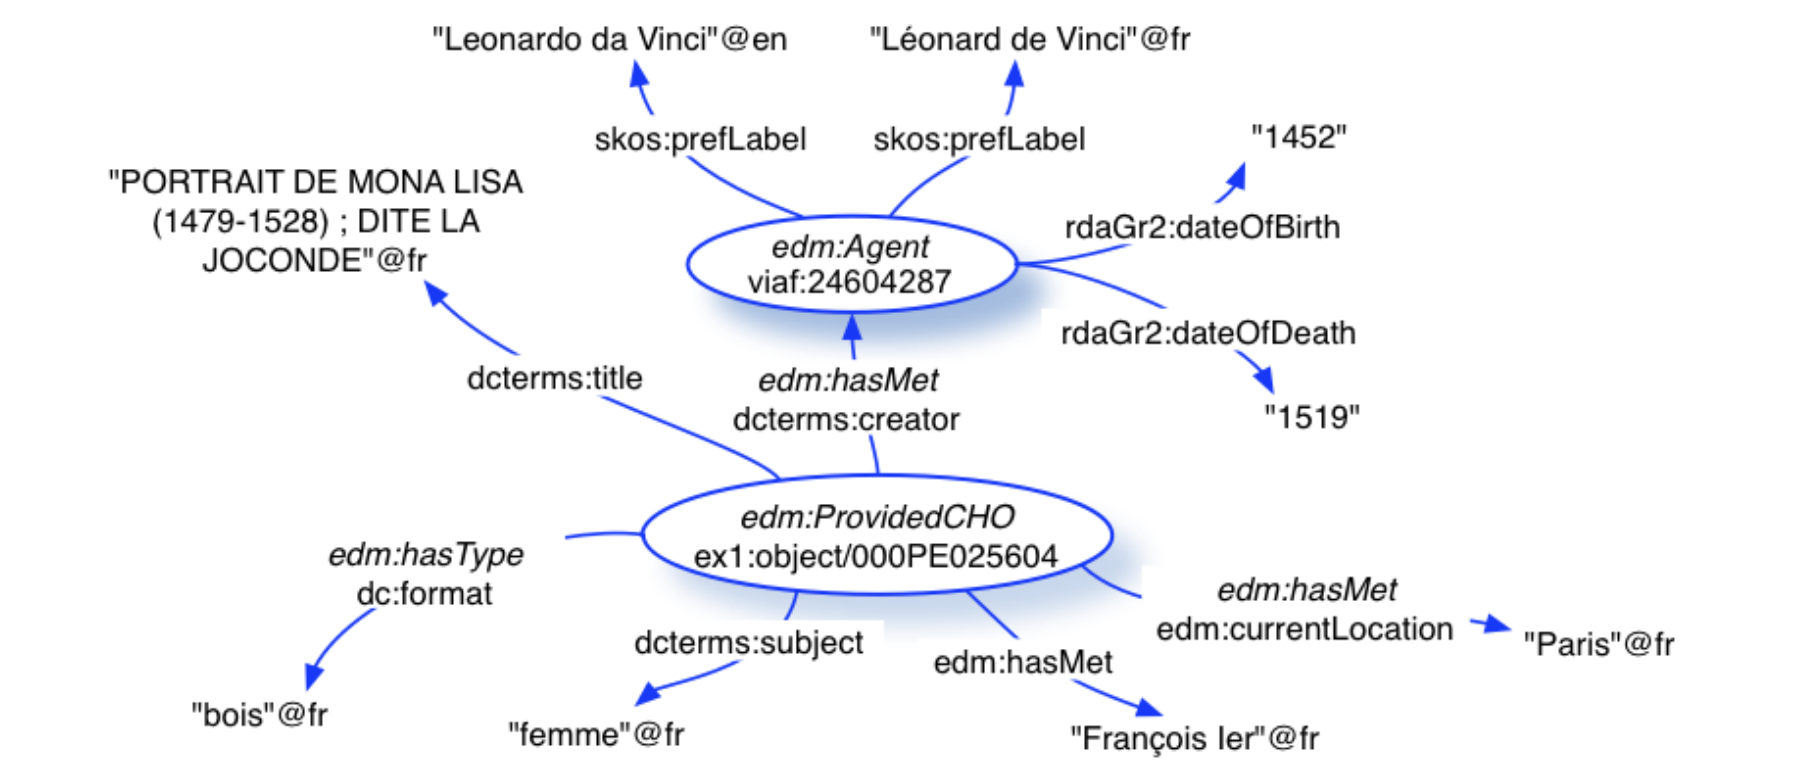
\includegraphics[width=15cm]{edm}
\caption{Extrait de \textit{Europeana Data Model Primer} ©Europeana.}
\end{figure}

Le web de données propose de nouvelles solutions, mais demeure une technologie avec certains défauts : il est très compliqué de faire face à un grand nombre de requêtes sur un corpus structuré selon le modèle RDF, et la création de liens entre les différents jeux de données est une pratique demandant beaucoup de temps pour son implémentation\footcite{rasmussen_pennington_connecting_2019}. Il faut plus que des données structurées en \gls{rdf} pour permettre un bon fonctionnement du web sémantique, la création de schémas de données de référence demeure un prérequis.
\begin{quotation}
[\textit{Traduction}]
Si chaque service web développe son propre schéma, cela équivaut à chaque ville et village développant leur propre borne d'incendie : il ne pourrait y avoir aucune collaboration entre les départements de pompiers, puisque les lances incendies ne fonctionneraient qu'avec leur borne locale. C'est seulement lorsque tous utiliseront les mêmes standards qu'une collaboration à grande échelle pourra être mise en place. \footnote{\textit{\inquote{If every web service developed its own schema for structuring its data, that would be the equivalent of every town and city developing its own type of fire hydrants : there could be no collaboration between fire departments because no department's hoses would fit any other department's hydrants. Only when everyone - or at least a significant portion of everyone - is using the same standards, is widespread collaboration possible}\cite[p.186]{pomerantz_metadata_2015}.}}
\end{quotation}

D'autres technologies travaillent à rendre interopérables les métadonnées des collections, à l'instar du protocole \gls{oai} ou des \gls{api}, qui permettent à des applications de communiquer entre elles\footcite{bermes_web_2013}. Les \gls{api}s sont des mécanismes très populaires pour accéder aux métadonnées sur les documents et aux documents eux-mêmes, elles sont dans la pratique presque davantage utilisées que les pages d'accueil des institutions\footcite{pomerantz_metadata_2015}. Les bibliothèques ont développé un standard très populaire spécifiquement dédié à l'interopérabilité des images, \gls{iiif}. Cette méthode de publication des données se base sur l'implémentation de différentes \gls{api}s et implique une structuration des métadonnées. Europeana a développé une extension de son modèle de métadonnées pour favoriser l'utilisation de \gls{iiif} par ses partenaires\footcite{iiif_consortium_home_nodate}.


%=====CONCLUSION TECHNIQUE

L'acquisition des compétences spécifiques pour les gestionnaires des collections numériques ne peut se limiter à la maîtrise d'une tâche, puisque la réussite du processus implique une vision d'ensemble et la prise de nombreuses décisions stratégiques (mise en place de standards de qualité pour la numérisation, définition des schémas de métadonnées, proposition d'un modèle, choix des outils pour favoriser l'interopérabilité etc.). \inquote{C'est tout une culture professionnelle du numérique qu'il faut élaborer et transmettre, de façon à permettre aux acteurs de s'inscrire dans un environnement global, de comprendre les implications de leurs choix et de leurs actions. \footcite[p.303]{claerr_manuel_2011}}. 

%=====ENJEU SUR LE CONTENU
\subsubsection{Enjeux sur le contenu}

Les collections numérisées sont disparates, proposant aux utilisateurs des ressources lacunaires ou contenant des doublons. Cela s'explique par des questions de financement, ou des questions de lois, de structures, de techniques\footcite{xie_discover_2016}\footcite{lopatin_library_2006}, mais également par le processus de sélection, du point de vue intellectuel, des ressources à numériser, et qui contribue à la problématique des silos. Les différentes stratégies de numérisation ont d'abord cohabité, développant pour chaque projet des critères propres, avant l'émergence des premières initiatives visant à les réunir. Bien que les critères de sélection intellectuels sont essentiels dans les entreprises de numérisation, ils n'ont jamais fait partie des contraintes de standardisation.\footcite{coutts_stepping_2017}.

Si les projets de numérisation de masse se sont construits dans la volonté de tout numériser et semblent à priori se passer de critères de sélection\footcite{lampert_ramping_2018}, la réalité est différente. Même si la sélection semble plus large, une prédominance des livres et des journaux dans les collections numérisées est à relever. De plus pour les \gls{agr}s que sont Europeana ou \textit{The Digital Public Library of America}, la sélection est fortement influencée par les collections et décisions des institutions partenaires, et par leurs positions géographiques. \footnote{La notion de \inquote{patrimoine européen} n'a pas attendu Europeana pour être diffusée à travers le monde. Le patrimoine des grandes bibliothèques américaines, numérisé par Google s'en est déjà chargé. C'est le patrimoine allemand, anglais, espagnol, français, italien de l'émigration européenne qui fonde les bases de celui des États-Unis. \cite{moatti_bibliotheque_2012}.} 

La vision de la bibliothèque universelle étant à priori issue du monde occidental et de la recherche, les plateformes d'accès aux produits de ces initiatives empêchent souvent leurs usages par des communautés ne partageant pas les mêmes normes\footcite{jones_public_2017}. Ce biais influence également la représentation des collections non occidentales dans les collections, qui suivent des formats de documents souvent mal pris en charge par les acteurs du marché\footcite{weiss_examining_2016}. 

Les projets de numérisation à plus petite échelle ne vont pas s'arrêter au profit des plus grands et l'intégration de ces collections signifie l'acceptation de leurs critères de sélection. \inquote{\textit{Digitisation work short of mass digitisation will continue, and selection criteria will be applied, whether in a structured or unstructured fashion\footcite[p.78]{coutts_stepping_2017}.}}

Le manque de normalisation pour la sélection peut sans doute être expliqué par le contexte et le développement rapide des projets de numérisation de masse, qui ont souvent \inquote{pallié au plus pressé} et se sont d'abord confrontés aux aspects techniques et légaux.

\begin{quotation}
[\textit{Traduction}] L'avancée de la numérisation a requis le développement et le renforcement de nombreux nouveaux éléments liés aux aspects techniques, structurels, légaux, financiers, au développement des interfaces de recherche. Ces aspects complexes évoluent de plus en plus rapidement, ce qui rend compréhensible le focus initial pour la création de standard et la coordination des pratiques associées. En conséquence, la mise en place de critères et d'aide à la sélection des ressources du point de vue de leurs contenus intellectuels a été négligé, alors même que ce champ d'étude était familier des acteurs de la culture et de l'information, habitués à les mettre en pratique dans la création de collections physiques.\footnote{\textit{\inquote{[...] the advent of digitisation required that many entirely new elements in the technical, infrastructural, discovery, preservation, legal and financial areas had to be developed, consolidated and matured. These were complex fields that changed rapidly. It is understandable that there was much emphasis on the creation of robusts standards and coordination of such practice; they were imperatives to apply the new technology effectively. As a consequence, guidance and criteria for the selection of content in terms of its intellectual value, a field that was already very familiar to information and heritage practitioners in relation to analogue materials, was somewhat overshadowed\cite[p.80]{coutts_stepping_2017}.}}}
\end{quotation}

Bien que les critères de sélection des objets à numériser se sont construits sans uniformisation, un groupe de critères communs émerge peu à peu. Margaret Coutts en propose huit, qui s'articulent en fonction du contexte des projets\footcite{coutts_stepping_2017}.
\begin{enumerate}
\item \textbf{L'accessibilité}

Les projets de numérisation se construisent autour de deux objectifs différents, celui de la préservation\footnote{Pour plus de détail, référez-vous à la section \ref{preservation}.}, et celui de l'accessibilité qui promet à la fois d'être élargie et enrichie par une publication en ligne. Ces deux notions font débat et dépendent fortement du contexte du projet.
\item \textbf{La notion de valeur}

Guidée par des critères intellectuels, historiques, physiques (format). Sélectionner en tenant compte de la valeur d'un document peut aussi être motivé par la notion de \inquote{valeur ajoutée}, découlant des nouveaux usages apportés par la version numérisée. La valeur est un choix subjectif qui dépend des intérêts des utilisateurs.

\item \textbf{La notion de rareté ou d'unicité}

Proposer pour la première fois la version numérisée. 

\item \textbf{La sélection thématique}

Une masse critique des documents numérisés est souvent atteinte par la mise en commun de plus petites entreprises, souvent articulées autour d'une thématique, d'un sujet particulier.

\item \textbf{Le format et le support}

Certains objets ont fait l'objet d'un numérisation plus rapide, à l'instar des livres, journaux, cartes et plans. 

\item \textbf{La cohérence}

Critère souvent utilisé lorsqu'il s'agit de mettre en commun différentes collections.

\item \textbf{La réunification virtuelle}

Permettant la réunification de ressources liées mais disséminées physiquement à travers différentes institutions.

\item \textbf{Le regroupement}

Propose un développement du critère précédent. Visant à réunir et enrichir des ressources déjà numérisées afin de développer de nouveaux services.

\end{enumerate}

Bernadette Dufrêne justifie la disparité des collections par leur développement initial autour de différents modèles, celui du musée où les pièces rares et trésors sont numérisés ; celui des archives où les documents sont numérisés selon une granularité d'ensembles thématiques liée à un fonds ; celui des bibliothèques, articulé souvent autour d'une charte documentaire détaillée visant à proposer la bibliothèque numérique idéale du chercheur et non élargir l'accès au patrimoine ; celui de Google, sans politique documentaire\footcite{dufrene_numerisation_2013}. Toutefois, l'absence de politique documentaire n'est pas forcément synonyme d'absence de critères de sélection comme nous l'avons vu plus haut.

Certains autres biais sont également listés, à l'instar des motivations des partenaires financiers qui peuvent venir imposer ou diriger certains choix, ou de la surreprésentation des collections des bibliothèques au détriment de celles des musées ou des archives, qui s'explique par un plus rapide développement de la numérisation dans ce secteur\footcite{coutts_stepping_2017}.

La croissance de la masse des données implique la mise en place de véritables directives dans la poursuite de la numérisation, afin de favoriser la réunification de ces données, d'éviter la redondance des collections et promouvoir la naissance de nouveaux usages\footnote{En Suède, un système de coordination a été mis en place par le bais de la Bibliothèque Nationale. \cite{dufrene_numerisation_2013}.}. 

 %===STOCKAGE
\subsection{Stockage sur le long-terme - préservation} \label{preservation}

Si la numérisation peut servir à préserver les objets physiques\footcite{xie_discover_2016}, la préservation signifie la maintenance sur le long-terme de l'accès aux objets numérisés ou à l'information contenue\footcite{coutts_stepping_2017}. Assurer cette longévité dépend de moyens techniques, économiques, légaux, organisationnels et structurels\footcite{xie_discover_2016}\footcite{georgetown_university_long_2009}. La prise en compte de cet enjeu est parfois laissée de côté dans les projets de numérisation de masse\footcite{lopatin_library_2006} alors que l'incertitude de pouvoir accéder sur la durée aux données a des impacts négatifs sur l'usage des plateformes et la conduite de projets de recherches dédiés\footcite{shankar_sustaining_2015}. 

Préserver implique souvent la copie de l'objet numérisé original, visant à la fois à servir de substitut et à proposer une version plus allégée pour les interfaces numériques\footcite{coutts_stepping_2017}. Les métadonnées de contexte sont importantes, puisque l'objet numérisé est souvent séparé de son format original dans le processus de numérisation\footcite{beaudoin_context_2012}.

Deux notions sont intrinsèques à la préservation, l'\inquote{intégrité} qui signifie que l'objet est le même que l'objet initialement numérisé, et l'\inquote{authenticité} qui consiste à s'assurer que l'objet est bien ce qu'il prétend être. La prise en compte de ces deux éléments doit assurer le long-terme de la compréhension et de l'usage de l'objet, alors même que les technologies seront modifiées\footcite{varniene-janssen_authenticity_2018}. 

En dehors de la question du stockage, on distingue trois technologies différentes pour la préservation des données\footcite{kowalczyk_digital_2018}. 
\begin{enumerate}
\item \textbf{La préservation des technologies de lecture}

Impliquant la conservation des anciens systèmes et des ordinateurs capables de les faire fonctionner.
\item \textbf{L'émulation}

Consiste à recréer un environnement technique capable d'exécuter les anciens programmes tout en fonctionnant avec une système moderne.

\item \textbf{La migration}

Passage d'un format de données vers un autre format. Souvent la méthode la moins coûteuse, mais implique certaines modifications de l'objet original, voir des pertes de données.

\end{enumerate}

Les technologies numériques présentent un paradoxe en terme de préservation. Ils multiplient les risques et les difficultés liés à la préservation sur le long-terme (dus à l'obsolescence des formats et programmes notamment) et proposent de nouvelles solutions et outils spécifiquement développés pour y pallier\footcite{xie_discover_2016}. 

Face aux difficultés posées par la préservation, de nouvelles pratiques voient le jour, visant à prendre en compte tous les aspects du cycle de vie des données (ajout de métadonnées standardisées, mise en place d'un plan de préservation, prise en compte des besoins des utilisateurs, valorisation et accessibilité) : la \gls{cur} de contenus numériques. Des infrastructures cross-institutions sont développées afin de partager les savoirs et les coûts\footcite{shankar_sustaining_2015}. Les bonnes pratiques développées pour le stockage des données ont conduits les dépôts institutionnels à devenir plus robustes, permettant à la fois l'ingestion de différents formats de données, leur organisation intuitive et proposant des fonctionnalités de recherche avancées\footnote{Le mouvement de l'\gls{os} a poussé les institutions a proposer des solutions efficaces pour les données de la recherche, qui peuvent être utilisées pour les projets de numérisation de masse. \cite{kowalczyk_digital_2018}.}. 

L'\gls{ue} a également financé des recherches visant à proposer des solutions de stockage sur le long-terme et des standards de métadonnées adaptés aux projets de numérisation de masse et leurs collections de données hétérogènes\footnote{Par exemple, le \textit{Scalable Preservation Environments} ou SCAPE projet, conclu en 2014.}\footcite{jurik_bridging_2015}.
\newpage
\subsection{Résumé des enjeux de la numérisation}
\begin{table}[H]
\centering
\begin{tabular}{|l|l|}
\hline
\rowcolor[HTML]{2E1A46} 
{\color[HTML]{FFFFFF} \textbf{Enjeux}}                                                                                   & {\color[HTML]{FFFFFF} \textbf{Résumé}}                                                                                                                                                                                                                                                                                                                                                                                                                                                                                                                                                                                                                                                                                                                                                                    \\ \hline
{\color[HTML]{2E1A46} \textbf{\begin{tabular}[c]{@{}l@{}}Amener différents\\ acteurs à collaborer\end{tabular}}}         & \begin{tabular}[c]{@{}l@{}}Susceptible d'impacter tous les autres enjeux, une collaboration \\ de qualité doit être mise en place entre les différents partenaires.\end{tabular}                                                                                                                                                                                                                                                                                                                                                                                                                                                                                                                                                                                                                          \\ \hline
{\color[HTML]{2E1A46} \textbf{\begin{tabular}[c]{@{}l@{}}Financement et \\ partenariats \\ public-privé\end{tabular}}} & \begin{tabular}[c]{@{}l@{}}Les coûts élevés impliquent des fonds privés. Ces partenariats \\ suscitent des craintes et manquent d'encadrement. Peu d'argent \\ est dédié à la préservation sur le long-terme.\end{tabular}                                                                                                                                                                                                                                                                                                                                                                                                                                                                                                                                                                                \\ \hline
{\color[HTML]{2E1A46} \textbf{Droit d'auteur}}                                                                           & \begin{tabular}[c]{@{}l@{}}Projets souvent limités aux \oe{}uvres libres de droit. Cela coûte cher\\ de rechercher les détenteurs de droits. Les \oe{}uvres du 20\up{e} siècle \\ sont sous-représentées. Pas de cadre légal européen, mais de \\ nombreux régimes nationaux. Réflexions autour de la directive sur \\ les \oe{}uvres orphelines et la prise de risques.\end{tabular}                                                                                                                                                                                                                                                                                                                                                                                                                                                          \\ \hline
{\color[HTML]{2E1A46} \textbf{\begin{tabular}[c]{@{}l@{}}Sortir des silos : \\ enjeux techniques\end{tabular}}}          & {\color[HTML]{333333} \begin{tabular}[c]{@{}l@{}}L'objectif est de rassembler des collections de provenances \\ différentes et permettre leurs interrogations en-dehors du silo de\\ leurs institutions.\\ Nécessité de fixer des standards pour la numérisation, et de définir \\ des critères de qualité.\\ Nécessité de fixer des standards pour les métadonnées, \\ présentation des différentes typologies, du rôle du schéma et de la\\ place des vocabulaires contrôlés.\\ Présentation des quatre principes du web sémantique et usages du \\ RDF, introduction d'autres outils favorisant l'interopérabilité \\ (OAI-PMH, APIs, IIIF).\\ Face à ces enjeux techniques en constante évolution, il est \\ nécessaire de développer la formation des gestionnaires de \\ collections.\end{tabular}} \\ \hline
{\color[HTML]{2E1A46} \textbf{\begin{tabular}[c]{@{}l@{}}Sortir des silos : \\ enjeux sur le \\ contenu\end{tabular}}}   & \begin{tabular}[c]{@{}l@{}}Un processus de sélection intellectuel non coordonné, qui \\ contribue à la création de collections disparates et redondantes\\ et ne favorise pas la mise en commun des collections. Nécessité\\ de mettre en place des directives et de prendre conscience des \\ typologies derrière ces critères de sélection (valeur, format, \\ unicité, accessibilité, thématique, cohérence, réunification \\ virtuelle, regroupement).\end{tabular}                                                                                                                                                                                                                                                                                                                                   \\ \hline
{\color[HTML]{2E1A46} \textbf{\begin{tabular}[c]{@{}l@{}}Stockage sur le \\ long-terme - \\ préservation\end{tabular}}}  & \begin{tabular}[c]{@{}l@{}}Préserver l'accessibilité sur le long-terme des données \\ numérisées afin d'en favoriser l'usage. Différentes méthodes \\ (émulation, préservation des technologies, migration) et systèmes\\ permettent la mise en place de cette préservation. Le coût reste\\ élevé, et les projets sont souvent construits sans plan de \\ préservation.\end{tabular}                                                                                                                                                                                                                                                                                                                                                                                                                     \\ \hline
\end{tabular}
\caption{Résumé des enjeux de la numérisation}
\end{table}   
\newpage

%====================CHAPITRE 3 (keyword context)
\chapter{Contexte du projet Time Machine}

Pour comprendre l'articulation du projet Time Machine au sein de l'histoire des projets de numérisation de masse et les réponses apportées aux enjeux liés à l'envergure de ces initiatives, il nous faut premièrement introduire le contexte du projet. Nous tenterons de définir dans le troisième temps de ce mémoire, si ses objectifs et solutions l'inscrivent dans une démarche de continuité ou contribuent à positionner les entreprises de numérisation de masse en tant que nouvel acteur de l'information. 

Cette présentation du cadre décrit d'abord le contexte académique de l'\gls{epfl} et de la recherche en humanités numériques qui l'ont vu naître, puis le projet \textit{Venice Time Machine} et les diverses activités du \gls{dhlab}, racines des développements futurs.

Nous terminons ce chapitre par une présentation de Time Machine, ses objectifs et  son organisation au moment de commencer notre stage.

Nous décrirons plus précisément notre mission de stagiaire et la réponse apportée par Time Machine aux enjeux de la numérisation dans la troisième partie de ce mémoire.

\section{La recherche en humanités numériques} 
%(keyword digitalhumanities)
\inquote{Nouveau} domaine d'étude, dont l'appellation est apparue au tournant des années 2000, les \textit{digital humanities (DH)}, humanités digitales ou humanités numériques pour les chercheurs francophones \footnote{Nous privilégions l'emploi du terme humanités numériques dans ce mémoire, qui est l'appellation utilisée en France, lieu de notre soutenance.}, proposent des programmes de recherche en cooccurrence avec les technologies informatiques et les différentes disciplines des sciences humaines.\footnote{\cite[p. 2]{meunier_paradoxe_2019}} Si les tentatives de définition abondent et demeurent volontairement larges, c'est aussi par refus d'établir \og une définition qui préexisterait à l'usage\fg{}\footnote{\cite[p. 2]{caraco_les_2012}}. 

Notre stage se déroulant au sein d'un laboratoire d'humanités numériques, il nous semble pertinent d'introduire quelques fondamentaux du domaine, pour mieux comprendre les origines académiques du projet Time Machine. Les débats étant à ce jour vifs parmi les communautés de chercheurs, dont les historiens, \og les réunions DH créent de nouveaux temps d'échange qui dépassent les thématiques et les périodes historiques, pour mettre en dialogue antiquisants, médiévistes, modernistes et contemporanéistes\fg{}\footnote{\cite[p. 5]{clavert_les_2019}}, nous ne prétendrons pas être exhaustif. 

Les humanités numériques constituent des zones d'échange, de projets à la frontière entre plusieurs disciplines, créant dans leurs pratiques de nouveaux espaces d'expression et leurs organisations associées, à l'instar d'Humanistica :  \textit{Association francophone des humanités numériques}, \footnote{\cite{association_francophone_des_humanites_numeriques_humanistica_nodate}} des conférences \gls{dh} Benelux \textit{\og an initiative that aims to further the collaboration between Digital Humanities activities in Belgium, The Netherlands, and Luxembourg \fg}{}\footnote{\cite{dhbenelux_2019_dhbenelux_nodate}}, des THATCamp \textit{\og The Humanities and Technology Camp \fg}{}\footnote{\cite{thatcamp_humanities_nodate}}, de Dariah en Europe \textit{\inquote{a pan-european infrastructure for arts and humanities scholars working with computational methods}}\footnote{\cite{dariah_digital_nodate}}, ou encore des conférence DH organisées par l'\textit{\og Alliance of Digital Humanities Organizations\fg}{}\footnote{\cite{alliance_of_digital_humanities_organizations_about_nodate}}.

La variété des approches est grande et diffère en fonction des rôles spécifiques attribués à l'expert des humanités ou à l'expert de l'informatique. Dans le premier type d'approche, les humanités numériques sont la suite des études menées en humanités, le numérique étant alors un outil aux services de \textit{\inquote{what is important today is not that we are doing work with computers, but rather that we are doing the work of the humanities, in digital form.}}\footnote{\cite[p.17]{schreibman_new_2016}}. Dans le deuxième type d'approche, l'informaticien est expert, et les données une fois générées sont offertes aux interprétations des chercheurs en humanités \footnote{\cite{meunier_paradoxe_2019}}. Cette situation a été identifiée par Jean-Guy Meunier comme le paradoxe des humanités numériques, lorsque les experts techniques estiment que \inquote{les traitement interprétatifs manquent de rigueur et de scientificité}\footnote{\cite[p.6]{meunier_paradoxe_2019}} et que les experts en humanités considèrent toute formalisation comme trop réductrice et peu capable de \inquote{rendre compte adéquatement de la complexité des objets traités} \footnote{\cite[p.6]{meunier_paradoxe_2019}}. La recherche en humanités numériques est dès lors une démarche complexifiée par les questions de compréhension et d'interprétation posées par ses objets d'étude, \inquote{d’autant qu’il n’y a pas une, mais des communautés \gls{dh}, qui distinguent notamment des approches anglo-saxonnes et européennes}\footnote{\cite[p.41]{clavert_les_2019}}. Pour le Professeur Willard McCarthy \footnote{Professeur au sein du département des humanités numériques du King's College de Londres.}, ce n'est pas uniquement le champ qui doit être interdisciplinaire, mais les personnes qui le pratiquent qui devraient tendre à l'être, se tenir informées de ce qui se fait ailleurs pour enrichir leurs expériences de recherche\footnote{\cite{schreibman_new_2016}}. Certains experts proposent une cartographie des champs de recherche : 

\begin{quotation}La variété des approches en \gls{dh} peut répondre à des interrogations en termes à la fois de recueils et gestion des sources de données, d'analyse et de représentation via des outils numériques - comme l'usage ou la constitution de bases de données, de cartographie de liens, d'étude sémantique ou lexicale etc. - ou encore de valorisation, notamment dans le cadre de l'histoire numérique publique.\footnote{\cite[p.35-36]{clavert_les_2019}}\end{quotation}

Si les démarches en humanités numériques sont multiformes et se distinguent de \inquote{tout un champ d'expérimentation croisant SHS et informatique (\textit{literary / linguistic / humanities computing}}\footnote{\cite{mounier_lou_nodate}}, les ancêtres de la discipline semblent communément acceptés, à l'instar du père Roberto Busa, jésuite pionnier de la numérisation et de l'analyse de corpus et de Franco Moretti, auteur de \textit{Graphes, cartes et arbres. Modèles abstraits pour une autre histoire de la littérature, 2008}, qui reste une référence pour son concept de lecture distante.\footnote{\cite{gefen_humanites_2017}} La \textit{Text Encoding Initiative (TEI)}, créée en 1987, figure aussi en bonne position puisqu'elle place les données au centre de son étude et s'adapte aux évolutions des outils informatiques.\footnote{\cite{clavert_les_2019}}. D'autres précurseurs communs aux projets de numérisation de masse pourraient figurer dans ce palmarès, notamment Paul Otlet, et Ted Nelson l'inventeur de la notion d'hypertexte.\footnote{\cite{clavert_les_2019}} Les projets en humanités numériques s'offrent à la fois comme outil et objet d'étude, tant leurs histoires s'écrivent au présent. 

\begin{quotation} [...] les humanités numériques ont permis l'émergence d’un vaste et riche patrimoine numérique, sources primaires de leur propre histoire que les historiens pourront très clairement exploiter, par l’hybridation de leurs outils maîtrisés de longue date (la lecture proche) avec ceux des \textit{digital humanities}, au premier rang desquels la lecture distante jouera un grand rôle.\footnote{\cite[p.43]{clavert_les_2019}}\end{quotation}

Time Machine fait de la question de la \gls{num} de masse l'un de ces enjeux. C\oe{}ur de nombreux projets en humanités numériques, l'acte de numérisation articule plusieurs moments (choix de la collection, conversion des documents papiers en versions électroniques, traduction du format électronique en format binaire, reconstruction de la structure du document, identification des caractères etc.)\footnote{\cite{meunier_paradoxe_2019}} et dans une même entreprise voient se confronter les différents rôles attribués à l'expert des humanités ou à l'expert de l'informatique. 

\begin{quotation}Ainsi, pour un expert des humanités, la constitution d’un corpus apparaîtra avant tout comme une activité de type herméneutique et l’ordinateur ne sera qu’un assistant, à l’inverse pour un expert de l’informatique, la numérisation apparaîtra avant tout comme l’application de technologies computationnelles d’une grande complexité.\footnote{\cite[p. 29]{meunier_paradoxe_2019}}\end{quotation}

Tout en s'inscrivant dans les démarches historiques des humanités numériques, Time Machine semble incarner les différents paradoxes de cette pensée académique au sein d'un même projet et promet de devenir à son tour objet d'étude de cette histoire.

\begin{quotation}Ainsi, au contact des humanités numériques, les historiens sont amenés à revisiter plusieurs aspects de la fabrique d’une histoire qui aujourd’hui articule productions individuelles et collectives, sous l’effet certes du numérique, mais aussi d’une culture du projet, qui innerve toutes les disciplines [...].\footnote{\cite[p. 42-43]{clavert_les_2019}}\end{quotation}

%-------------------------------------------------------------------------- keyword context
\section{Le Laboratoire d'humanités numériques de l'EPFL}
L'\gls{epfl} ouvre ses portes en 1853 sous le nom de l'École Spéciale de Lausanne. Au fil des années, l'école grandit, voyant de nouvelles spécialisations s'intégrer à son cursus (électricité, physique, architecture etc.), et d'une académie, devient université. Elle prend son nom actuel en 1969, année qui coïncide avec le début de son établissement sur le campus d'Écublens-Dorigny (Suisse). Réputés sélectifs, les cursus ne désemplissent pas et l'offre continue de croître. Dès 1991, la construction d'un parc scientifique hébergeant une dizaine de compagnies favorise le développement des activités de recherche. En 2003, année de son 150\up{ème} anniversaire, l'école compte plus de 6000 étudiants. 2014 marque la création de deux nouveaux campus en Suisse avec l'ouverture de l'\gls{epfl} Valais\footnote{\cite{epfl_epfl_nodate-1}} (dix laboratoires actifs dans les domaines de l'énergie, de l'environnement et de la santé) et de l'\gls{epfl} Fribourg\footnote{\cite{epfl_epfl_nodate}} (\textit{\og smart living lab \fg{}}  dédié aux recherches en technologies de la construction, bien-être et comportements, interaction et processus de conception, et systèmes énergétiques). En 2015, le nombre d'étudiants franchit la barre des 10'000\footnote{\cite {epfl_history_nodate}}.

En 2019, l'\gls{epfl} compte cinq facultés, trois collèges, plus de 11'000 étudiants, et quelques 210 compagnies constituent son parc scientifique\footnote{\cite {epfl_innovation_nodate}}. Son rayonnement s'étend à l'international, l'\gls{epfl} est en bonne position dans les classements universitaires européens et mondiaux.

Fondé en 2002, le Collège des Humanités (CDH) est un  un \og lieu de convergence des sciences humaines et sociales au coeur de l'\gls{epfl}, basé sur le concept de \gls{poly}, reflétant la nécessité pour les futurs ingénieurs et scientifiques d'adopter une perspective pluraliste face aux enjeux auxquels ils sont confrontés\fg{}\footnote{\cite {epfl_vision_nodate}}. Les perspectives s'organisent autour de quatre grandes thématiques : l'interdisciplinarité, la conscience globale (comprendre l'histoire des technologies pour mieux les faire évoluer), la citoyenneté et la créativité (engagement à travers l'art et la production artistique). La recherche au sein du CDH se compose de deux instituts, le \textit{Digital Humanities Institute (DHI)} et l'\textit{Institute for Area and Global Studies (IAGS)}, et d'un pôle soutenant des projets transdisciplinaires entre l'Université de Lausanne (UNIL) et l'\gls{epfl} : le \textit{Collaborative Research on Science and Society (CROSS)}\footnote{\cite {epfl_cross_nodate}}. Le CDH coordonne également le programme d'enseignement en sciences humaines et sociales pour tous les étudiants de l'\gls{epfl} et le DHI propose un master en humanités digitales et est lié au programme doctoral en humanités digitales \footnote{\cite {noauthor_formations_nodate}}.

Le \gls{dhlab} dans lequel nous avons effectué notre stage, constitue l'un des trois laboratoires du DHI, aux côtés du \textit{Digital and Cognitive Musicology Laboratory (DCML)} et du \textit{Laboratory for Experimental Museology (eM+)} et de plusieurs groupes thématiques de recherche (\textit{Social Computing Group},\textit{ Social Media}).\footnote{\cite {epfl.dhlab_dh_nodate}} 

Le \gls{dhlab} est fondé en 2012 par le Professeur Frédéric Kaplan avec pour objectif de développer de nouvelles approches informatiques pour l'étude du passé et la découverte du futur. Le Professeur Kaplan est également le créateur du Master en humanités digitales du DHI et co-organisateur de la \textit{Digital Humanities 2014}, conférence internationale de l'\textit{Alliance of Digital Humanities Organizations (ADHO)}\footnote{\cite {epfl.dhlab_dh_2019}} à Lausanne, qui demeure l'un des plus grands rassemblements scientifiques du domaine. 

\begin{figure}[H]% force à placer l'image au sein de notre balise figure
\centering
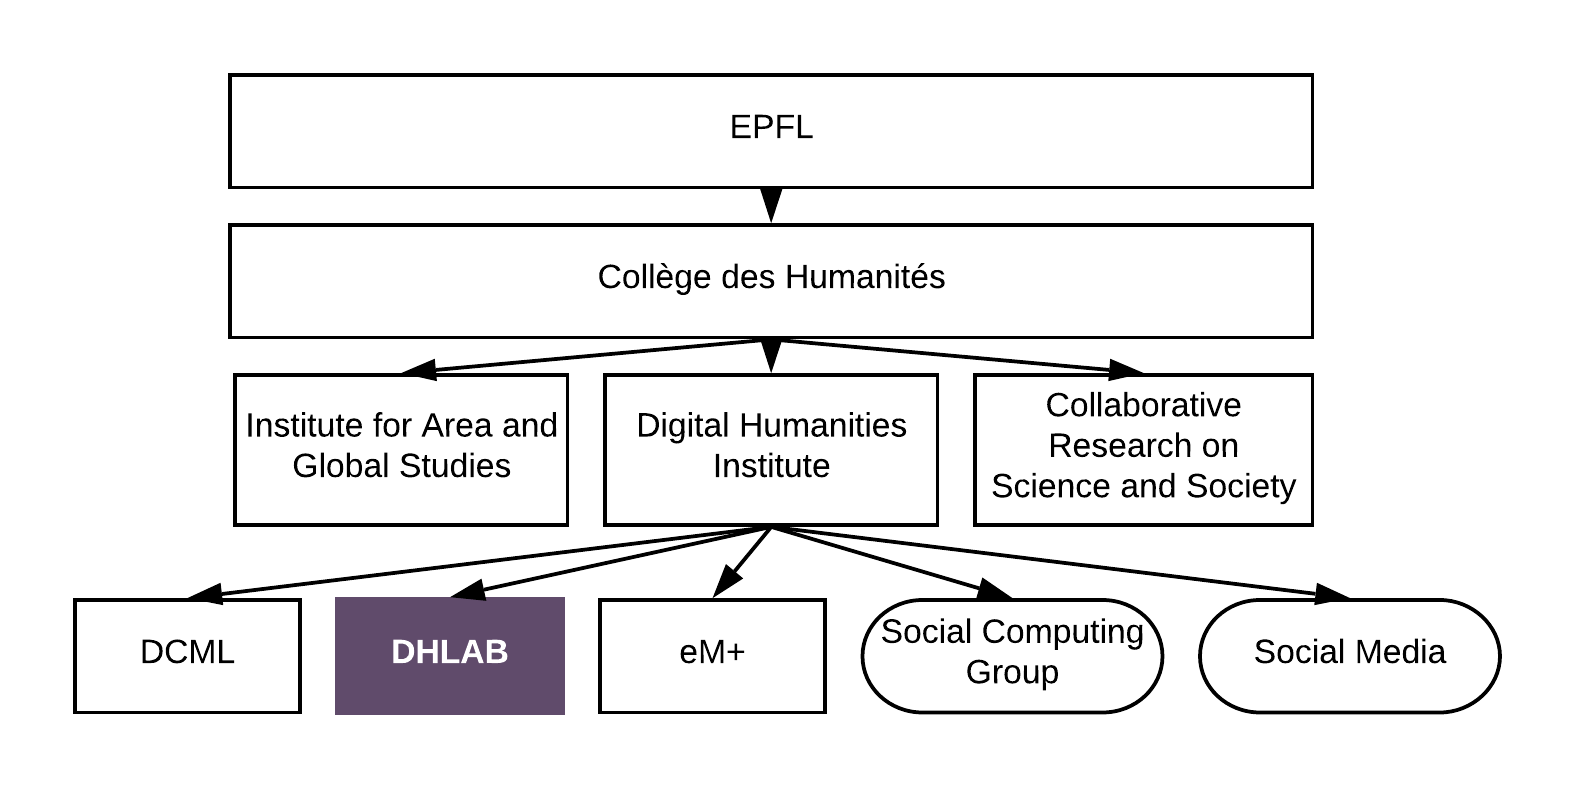
\includegraphics[width=15cm]{dhlab.png}
\caption{Le \gls{dhlab} au sein de l'\gls{epfl}}
\end{figure}

\section{Venice Time Machine}
Né de la crainte de voir les informations non digitales tomber dans \inquote{les oubliettes de l'histoire}\footnote{\cite{dubuc_venice_2017}}, initié en 2012 par l'\gls{epfl} et l'université Ca'Foscari de Venise, le projet vise à construire un modèle multidimensionnel de Venise et de ses évolutions, sur une période de 1000 ans : une machine à remonter le temps. Conscients dès le départ que les enjeux du projets nécessitent bien plus que de la puissance de calcul informatique, les initiateurs s'allient le secours d'historiens et d'archivistes pour mettre en place les processus de \gls{num}\footnote{\cite{abbott_time_2017}}. La transformation des 80 kilomètres d'archives vénitiennes en un système d'informations nécessite en plus un grand travail d'indexation et de cartographie pour aboutir à ce qui se veut une version augmentée de \textit{Google Maps}, offrant en plus un ancrage temporel\footnote{\cite{world.minds_frederic_nodate}} : un croisement entre histoire et \textit{\gls{bigd}}\footnote{\cite{rts_remonter_nodate}}. 

Les archives numérisées par le projet proviennent de deux sources différentes\footnote{\cite{evangelista_time_2018}} : 
\begin{itemize}
\item \textbf{Les Archives d'Etat de Venise} : en 2018, 190'000 documents avaient été numérisés
\item \textbf{La Fondation Cini} : la Fondation possède un million de photos d'art, en 2018 quelques 720'000 documents photographiques avaient été numérisés
\end{itemize}
Face à d'immenses corpus souvent manuscrits, les outils permettant la lecture automatique sont cruciaux. L'EPFL rejoint le projet européen \textit{Recognition and Enrichment of Archival Documents (READ)}\footnote{\cite{noauthor_recognition_nodate}} poursuivant des objectifs similaires, et emploie une partie de ses équipes à développer des solutions d'\gls{appauto}\footnote{\cite{nature_video_virtual_nodate}}. 

Avec le projet vénitien, l'\gls{epfl} souhaite développer, tester et démontrer l'efficacité d'une méthode appelée à se déployer avec Time Machine à travers l'\gls{ue}\footnote{\cite{arte_venice_nodate}}. Sans le succès du Venise Time Machine, il n'y a pas de Time Machine\footnote{\cite{kaplan_cartographie_2018}}. 

\subsection{Développements technologiques}
Le projet se poursuivant actuellement, de nombreux outils, techniques, méthodologies ont été spécialement dédiés à son avènement. En plus de la \gls{num}, il a fallu apprendre aux ordinateurs à automatiquement extraire certains types d'information, ce qui a impliqué un grand travail d'indexation manuelle. Tous ces éléments viendront enrichir la future interface de Time Machine et contribueront à la création de ce \textit{\gls{bigd}} du passé. L'envergure de ce projet étant trop vaste pour en lister tous les composants, voici un aperçu de leurs variétés :

\begin{itemize}
\item \textbf{The Replica Scanner} : numériser massivement a induit à  la création de divers scanners. Celui-ci, développé avec Adam Lowe de Factum Arte\footnote{\cite{s.l_factum_nodate}} est capable de numériser un document photographique recto verso toutes les quatre secondes.
\item \textbf{DhCanvas} : moteur de recherche associé aux documents numérisés, permettant la recherche dans le document original et son contenu,  fonctionnant comme un outil participatif de transcription. Les utilisateurs autorisés peuvent corriger les erreurs d'extraction\footnote{\cite{evangelista_time_2018}}.
\item \textbf{Replica} : une interface de recherche spécialement dédiée aux fonds des images numérisées de la Fondation Cini, proposant une recherche visuelle (par motifs, position des personnages etc.) et textuelle des documents et permettant d'établir des connections entre des images\footnote{\cite{evangelista_time_2018}}.
\item \textbf{Venice Scholar} : travail consacré aux ouvrages et journaux scientifiques vénitiens numérisés et dont les citations ont été automatiquement extraites, pour pouvoir étudier l'historiographie vénitienne\footnote{\cite{evangelista_time_2018}}.
\item \textbf{DhSegment} : confronté à l'enjeu de traiter l'immense masse des images numérisées, ce système se base sur les \gls{reneu} pour en extraire automatiquement certaines parties (lignes, encadrés, zone de texte etc.)\footnote{\cite{epfl.dhlab_introduction_nodate}}.
\end{itemize}

\begin{figure}[H]% force à placer l'image au sein de notre balise figure
\centering
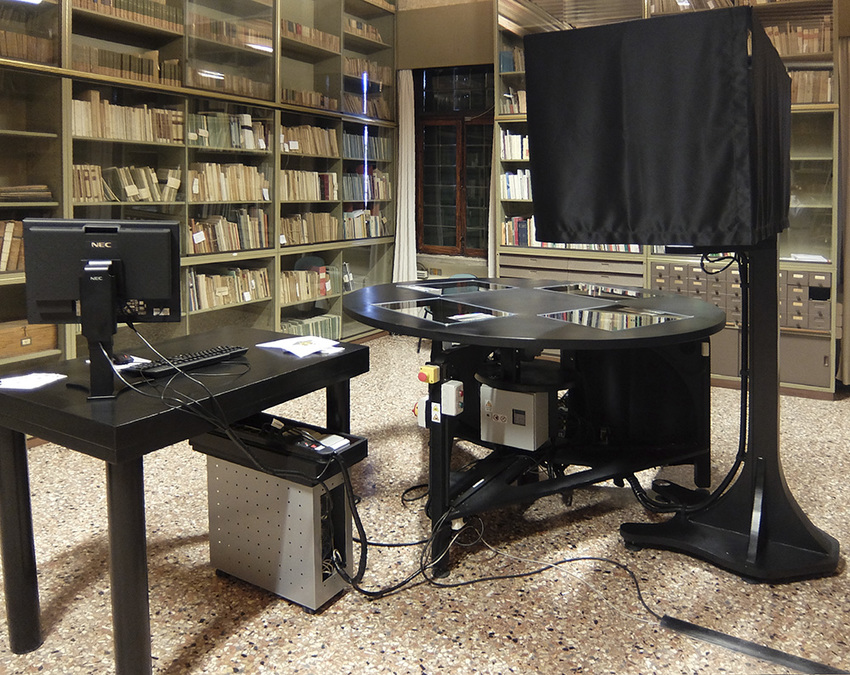
\includegraphics[width=15cm]{replica_scanner.jpg}
\caption{Le scanner Replica à la Fondation Cini, \textit{© Copyright 2019 Factum Foundation}}
\end{figure}

\section{Le projet Time Machine}

Le 14 décembre 2016, Frédéric Kaplan, Professeur et occupant de la chaire d'humanités digitales de l'\gls{epfl}, publie dans le journal suisse \textit{Le Temps}, le \href{https://www.letemps.ch/opinions/leurope-construire-premiere-time-machine}{manifeste} du projet Time Machine. L'intérêt du public et des institutions patrimoniales pour le projet Time Machine s'éveille et l'aventure est officiellement lancée ; Time Machine peut se lancer à la conquête de l'Europe et créer sa \inquote{machine à remonter le temps}. 

\begin{quotation}
L’Europe a inventé le web. Le web est devenu la matrice d’un monde nouveau. Les acteurs qui, les premiers, en comprirent la logique, dominent aujourd’hui notre monde. Une trentaine d’années plus tard, le virage spatio-temporel de l’Internet, en plongeant l’information numérique dans un espace bien plus large, redéfinit les règles du jeu.

Le projet Time Machine peut donner à l’Europe la technologie de son renouveau: une occasion unique pour construire notre futur à partir de notre patrimoine commun, une occasion unique pour nous retrouver\footnote{\cite{noauthor_leurope_2016}}.
\end {quotation}

\begin{figure}[H]% force à placer l'image au sein de notre balise figure
\centering
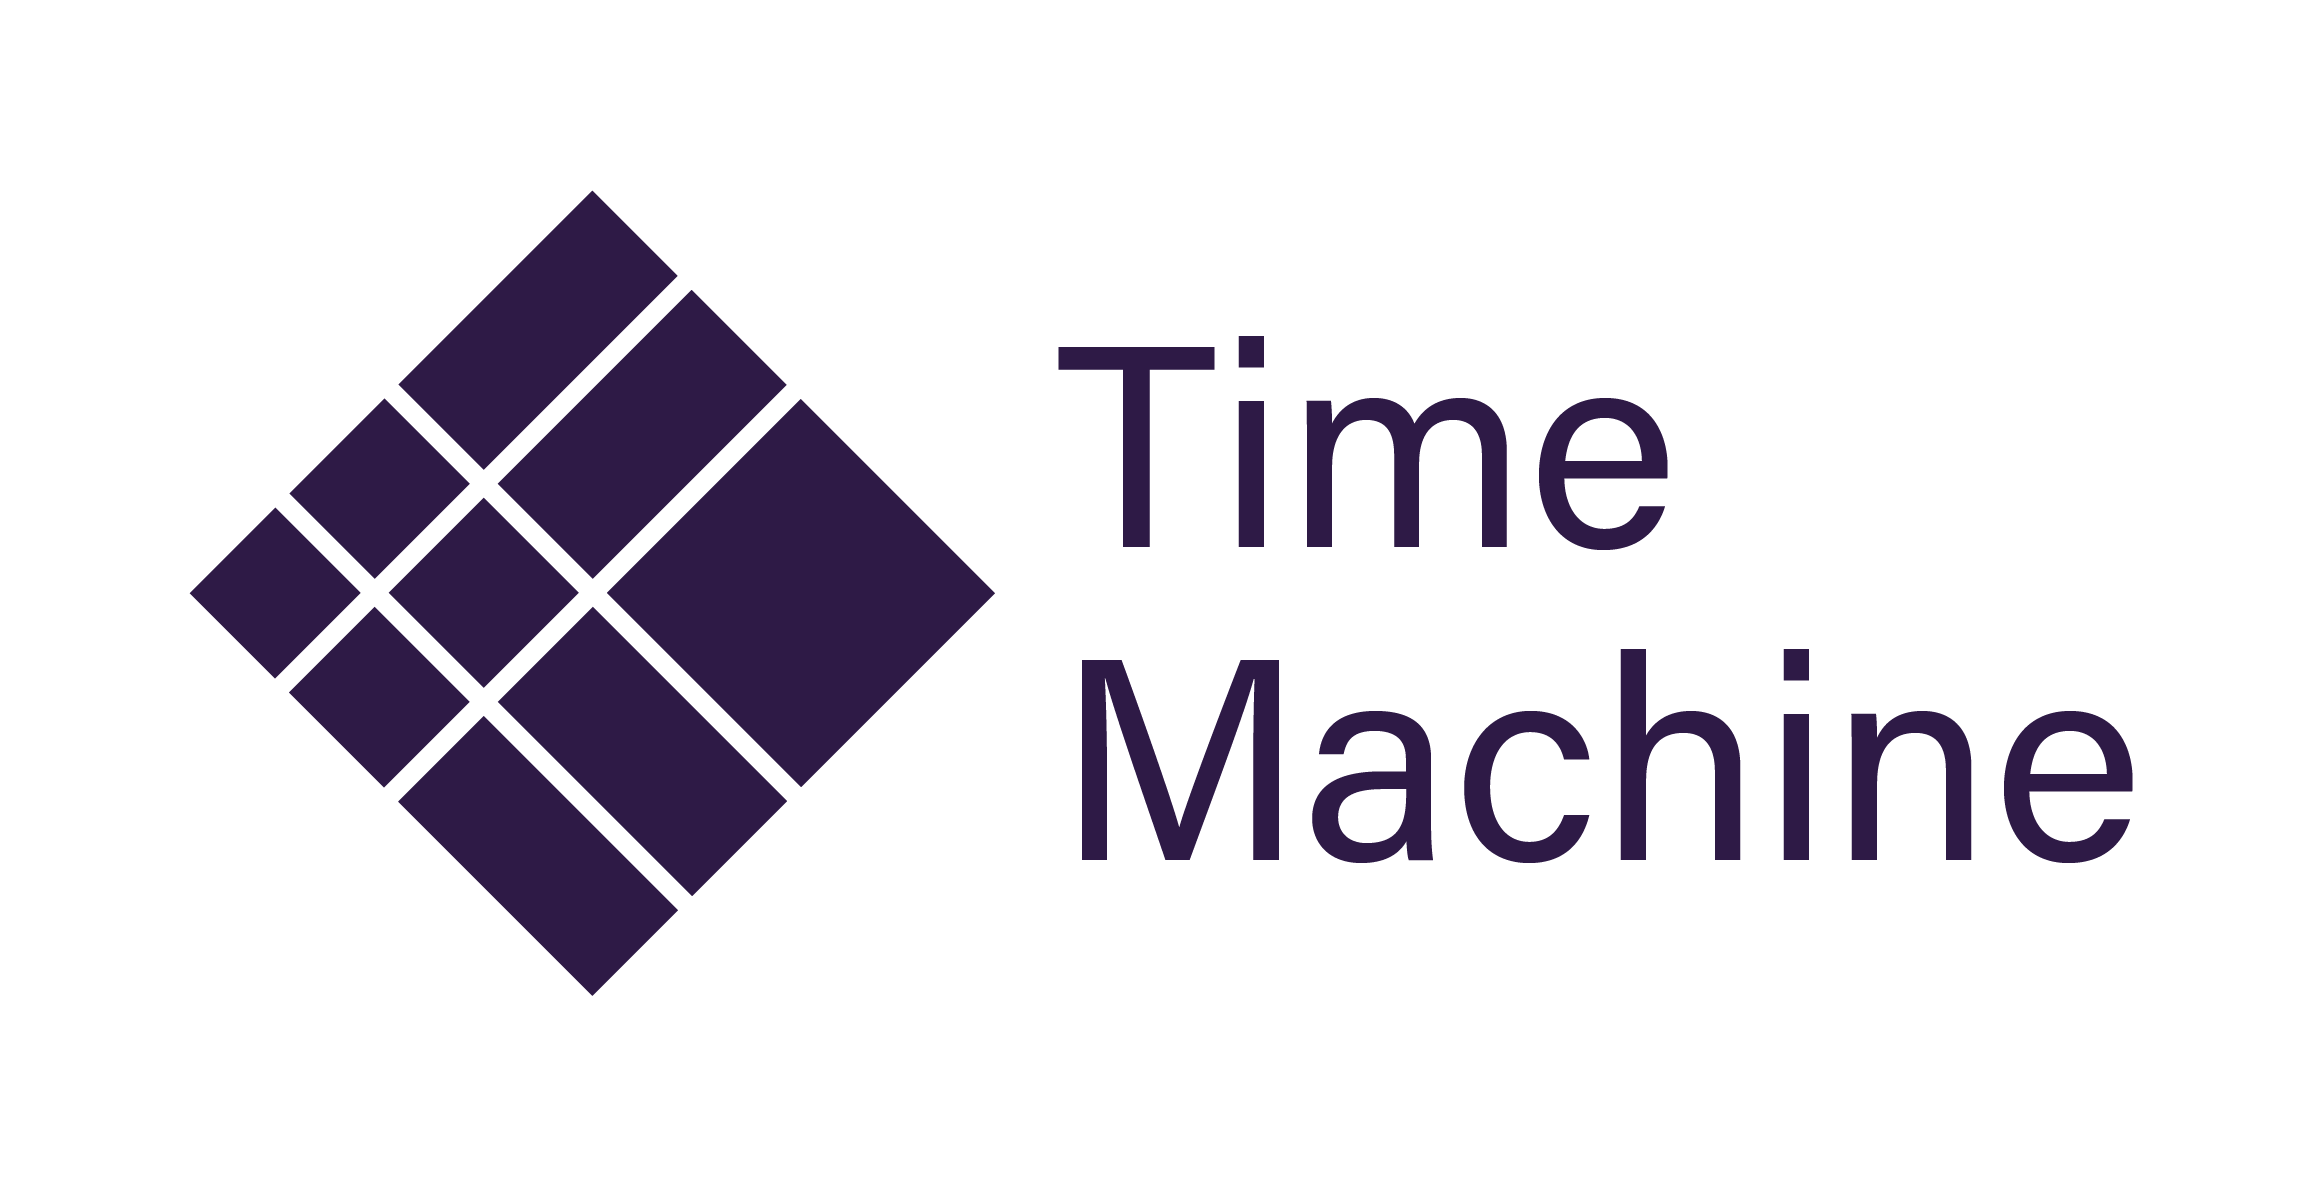
\includegraphics[width=15cm]{TM_logo.png}
\caption{Time Machine, logo \textit{© Copyright 2019 Time Machine}}
\end{figure}

\subsection{FET Flagships ou la recherche de financement}\label{fet}
A travers l'initiative des \textit{FET Flagships} ou \inquote{Initiatives-phare des technologies Futures et Emergentes}, la Commission européenne mettait au concours un soutien financier d'un milliard d'euros réparti sur dix ans. Les projets éligibles se devaient d'être visionnaires, de proposer des solutions scientifiques et technologiques innovantes et de réunir sur le long-terme autour d'un objectif commun et d'une feuille de route aux solutions ambitieuses, des équipes de recherche interdisciplinaires\footnote{L'\gls{epfl} pilote déjà un projet doté d'un tel financement, le \inquote{Human Brain Project}.}\footnote{\cite{moriscl_fet_2013}}. 

L'ambition de Time Machine s'accordant avec les objectifs fixés par la Commission, ses initiateurs (\textit{l'\gls{epfl} s'est alliée le concours de 32 partenaires pour développer et financer la proposition du projet, dont l'École Nationale des Chartes}) se sont lancés dans la course. L'histoire ne s'est pas faite sans embûches, Time Machine s'inscrivant sous le sigle de la culture, il fallut d'abord faire modifier les critères de sélection définis par l'\gls{ue} qui s'opposaient aux candidatures issues du milieu \footnote{\cite{rts_invite_nodate}}. En 2016, Time Machine est officiellement retenu comme candidat et en février 2019, le projet est classé premier parmi les six finalistes en lice pour la dernière ligne droite, avec cette fois une enveloppe d'un million d'euros et une année (à compter du 1er mars 2019) pour démontrer de l'organisation et de la faisabilité du projet.

Cette première victoire est nuancée, puisque coïncidant avec une année de votation, le programme de recherche européen \textit{Horizon Europe}, doté d'une enveloppe de quelque cent milliards d'euros pour la période 2021-2027, peine à se stabiliser \footnote{\cite{noauthor_crise_nodate}}. Le projet des FET Flagships est abandonné par la Commission européenne sans que pour l'heure une solution concrète ait été proposée aux six projets concurrents \footnote{\cite{rts_coup_2019}}. 

Nous avons commencé notre stage en cette période d'incertitude financière, étant à la fois contraints par l'\gls{ue} de planifier la mise en route du projet puisque le million a été perçu, mais sans certitude quant à l'ampleur finale du budget alloué.

\subsection{Time Machine, quels objectifs ?}

Dès 2014, le Professeur Frédéric Kaplan propose un modèle en forme de \inquote{champignon} pour expliciter l'ampleur des informations dont l'humain dispose pour évaluer une période donnée\footnote{\cite{ted_frederic_nodate}}. L'image est porteuse, plus l'on se rapproche du présent, plus le cône s'élargit. Face à une société désormais digitale, le risque est grand de perdre pour toujours l'accès aux informations contenues uniquement sous formes physiques, les enjeux liés à la conservation de ces documents sont réels, mais comment parvenir à rétablir un équilibre entre l'information du passé et l'information du présent\footnote{La \textit{factsheet} du projet, donnée en annexe \ref{factsheet}, offre une synthèse plus visuelle.} ? 

\begin{figure}[H]% force à placer l'image au sein de notre balise figure
\centering
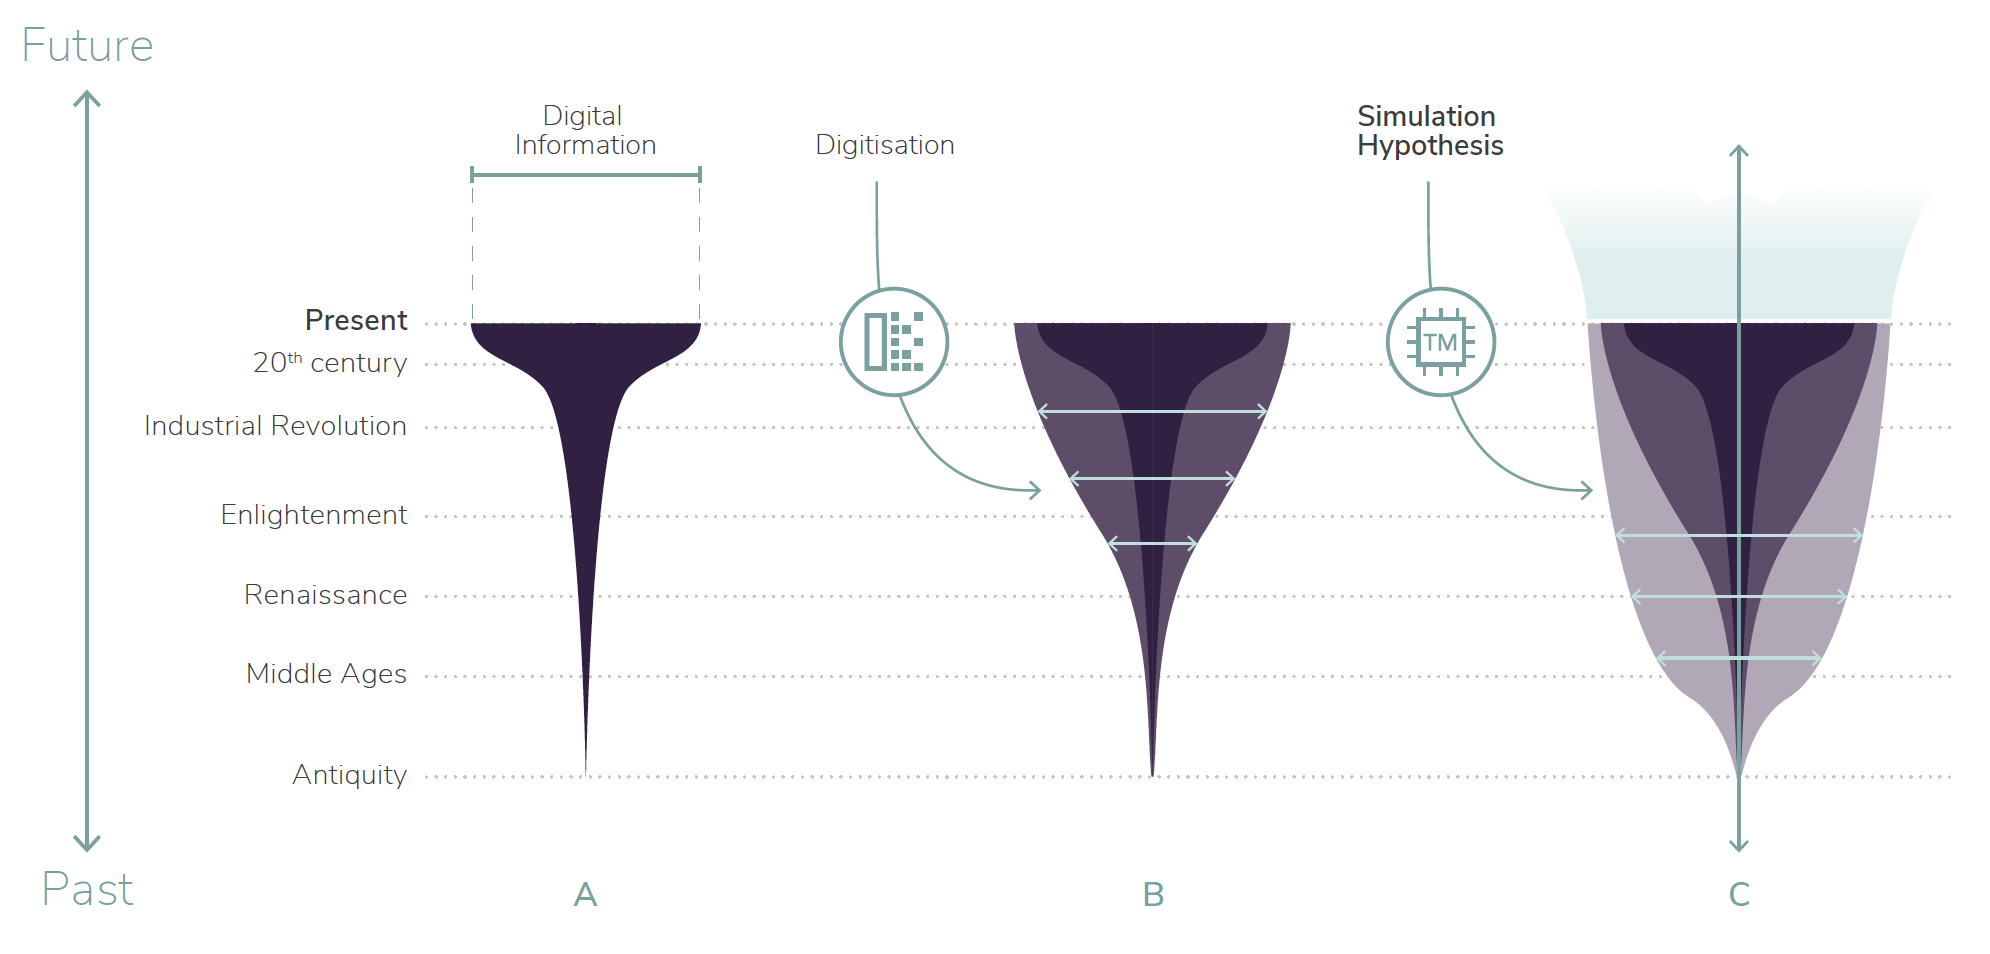
\includegraphics[width=17cm]{champ_info.png}
\caption{Time Machine, Information's Mushroom \textit{© Copyright 2019 Time Machine}}
\end{figure}

En visant comme résultat la création d'un \gls{graph} de données du passé, le \textit{\gls{bigd} of the past}, impliquant le développement de processus, technologies et innovations nécessaires à sa réalisation, Time Machine poursuit différents objectifs\footnote{Time Machine Manifesto, 2019 URL : https://documents.icar-us.eu/documents/2019/05/time-machine-manifesto.pdf} :

\begin{itemize}
\item Révolutionner les connaissances en \gls{ia} et dans le domaine des sciences de l'information et de la communication, positionnant l'Europe comme meneur sur le marché de l'extraction et de l'analyse d'énormes jeux de données hétérogènes et complexes, induits par les activités et réalisation passées et présentes du genre humain.
\item Offrir de nouvelles perspectives aux chercheurs en humanités et sciences sociales, leur permettant de positionner leurs objets d'étude à l'échelle plus large de l'histoire et de la culture européenne.
\item Devenir moteur et acteur de l'\textit{\gls{os}} et mettre à disposition les données du projet dans des dépôts ouverts et publics.
\item Offrir un flux de connaissances à l'enseignement, encourageant les réflexions sur le long-terme et l'apprentissage de la pensée critique.
\item Devenir un nouvel acteur économique, par la création d'emplois, services et produits appelés à influencer les secteurs clés de l'économie européenne.
\end{itemize}

\subsection{Quelle(s) méthode(s) pour Time Machine ?}

Créer un système d'information d'ampleur européenne basé sur un \gls{graph} de données du passé implique le déroulement de plusieurs étapes\footnote{\cite{ted_frederic_nodate}}\footnote{\cite{kaplan_cartographie_2018}} et le déploiement de technologies nécessaires à leurs succès. Se basant sur les innovations et méthodologies du projet vénitien, des projets menés en parallèle par l'équipe du \gls{dhlab}, et de ceux conduits par les partenaires du futur réseau, Time Machine entend mener ses révolutions technologiques à différents niveaux\footnote{Les partenaires étant actuellement plus de 300, il est impossible de rendre justice dans le cadre de ce travail à la multitude des projets en cours appelés à contribuer à la mise au point de Time Machine.} : 

\begin{enumerate}
%==========Première technologie ==================
\item \textbf{Numérisation massive des documents - archives - patrimoine bâti} 

Poursuivre le développement des outils de numérisation pour les documents (2D) et bâtiments (3D). 

Depuis 2018, l'\gls{epfl} conjointement avec la fondation Cini et Factum Arte\footnote{\cite{s.l_factum_nodate}} a créé un centre d'expérimentation et de formation aux techniques de numérisation à Venise : \textit{ARCHiVe, Analysis and Recording of Cultural Heritage in Venice}\footnote{\cite{noauthor_archive_nodate}}, diverses études sont en cours pour créer des scanners de nouvelles générations, mais également des programmes facilitant le suivi et l'automatisation des processus (traitement automatique de la post-production, ajout de métadonnées, indexation du texte). Les technologies d'\gls{appauto} sont utilisées par souci d'automatisation et de gain de temps. 

Les innovations apportées par ce \inquote{modèle} vénitien seront amenées par Time Machine, avec l'aide des acteurs locaux du marché de la numérisation, à se répandre et se développer à travers l'Europe, créant un réseau Time Machine de centres de numérisation européen. Cette uniformisation des processus permettra l'harmonisation des coûts et la garantie de la qualité des données. 

Une fois les données numérisées, leur stockage doit être assurés en vue de leur valorisation. Si un grand nombre d'institutions patrimoniales disposent de leurs propres serveurs, ce n'est pas forcément le cas des plus petites et ce n'était pas celui des archives vénitiennes. Une \textit{Time Machine Box}\footnote{\cite{epfl.dhlab_home_nodate}} a été développée, visant à accompagner les partenaires dans leurs démarches de numérisation et leur offrir une alternative de stockage en local.

La numérisation du patrimoine bâti implique l'utilisation des techniques de la \gls{photo} et l'alignement de différents nuages de points. L'ambition de Time Machine étant à l'échelle de villes, les technologies actuelles devront être améliorées. Le projet \textit{ScanVan (2016-2020)}, conduit par le \gls{dhlab}, a pour objectif le développement d'un véhicule capable de numériser les villes et de créer automatiquement des modèles 3D de ces territoires\footnote{\cite{epfl.dhlab_2016_nodate}}. 
\begin{figure}[H]% force à placer l'image au sein de notre balise figure
\centering
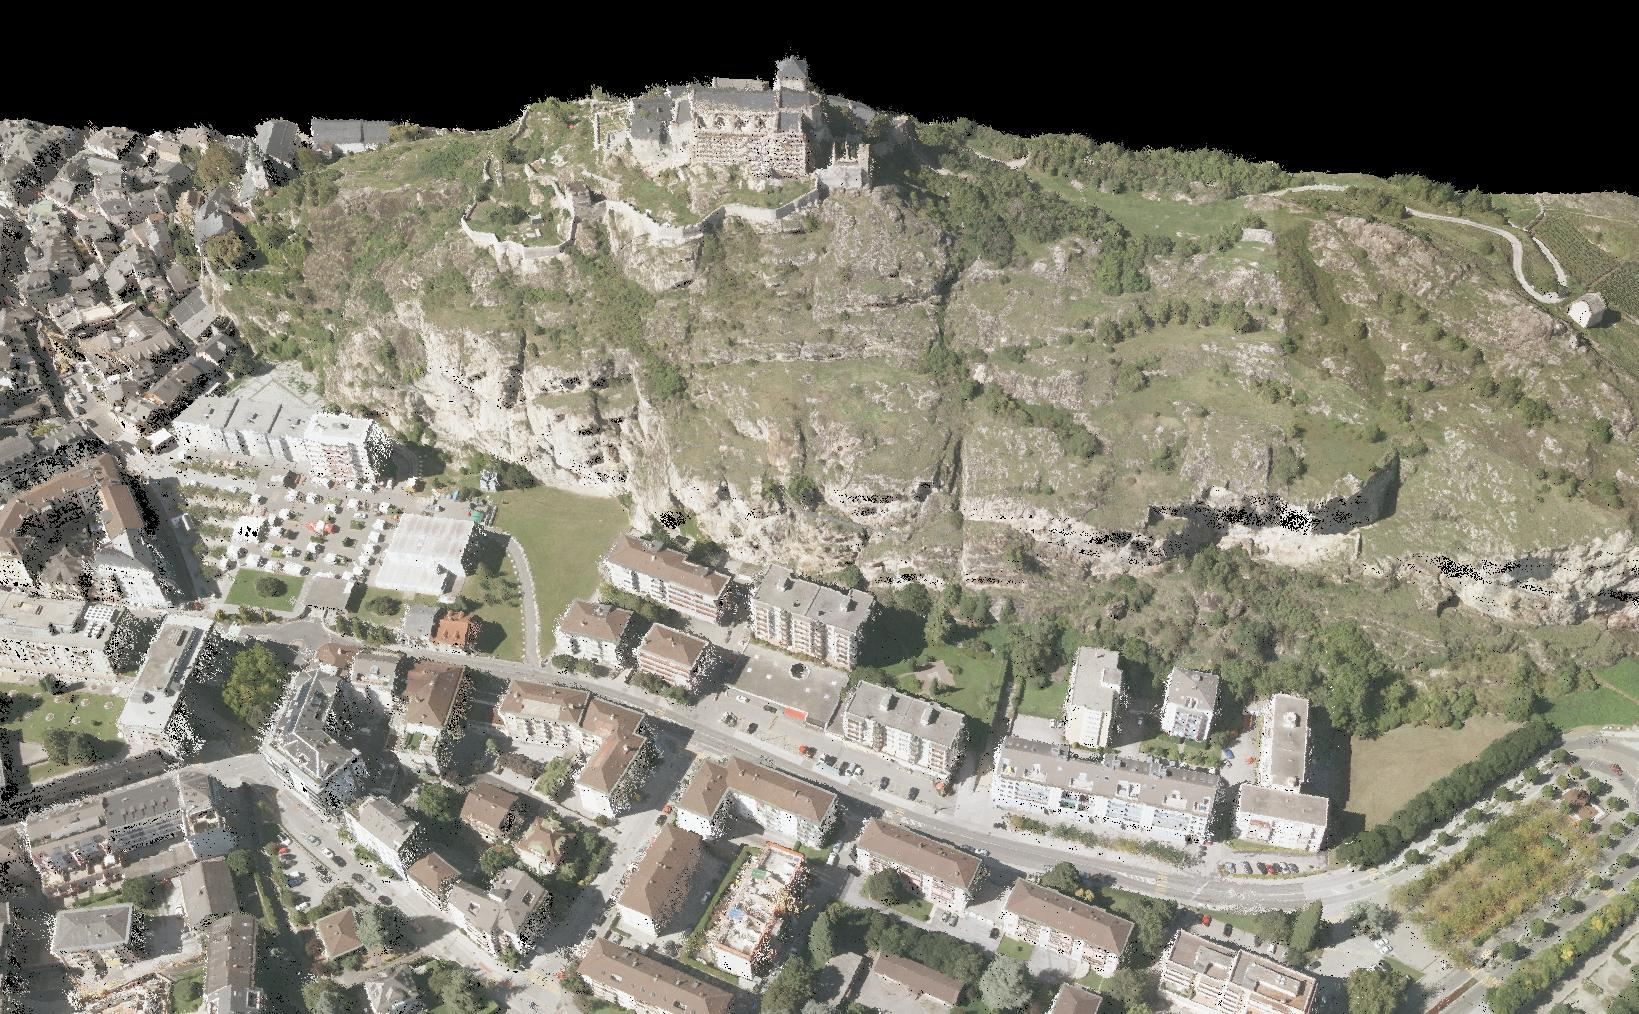
\includegraphics[width=15cm]{ScanVan.jpg}
\caption{Ville de Sion, compilée par ScanVan \textit{© Copyright EPFL DHLAB}}
\end{figure}
Iconem\footnote{\cite{iconem_iconem_nodate}}, start-up partenaire du projet, s'est spécialisée dans la numérisation de sites patrimoniaux en danger, grâce à des drones et à des processus de \gls{photo}. Par la mise en commun de ces développements technologiques, Time Machine vise à la création et à l'implémentation d'un système des plus efficients.
%==========Deuxième technologie ==================
\item \textbf{Extraction et indexation des informations contenues} 

On peut déterminer différentes étapes dans les traitements d'un document après sa numérisation et la liste tend à s'agrandir. On parle notamment : de l'automatisation des processus de repérages du texte ou des motifs au sein d'une image, de la compréhension de l'architecture du document par le biais des technologies du \gls{tal}, de la \gls{ree}, ou encore des technologies liées à la \gls{reo}.

 La plupart des projets du \gls{dhlab} conduisent des recherches dans ces domaines, c'est le cas notamment de \textit{DHSegment}\footnote{\cite{epfl.dhlab_introduction_nodate}} cité pour le projet vénitien ou du projet \textit{Impresso - Media monitoring of the past (2017-2020)}\footnote{\cite{epfl.dhlab_2017-2020_nodate}}, visant à automatiser l'extraction des informations de 200 ans d'archives de journaux afin d'en faciliter la recherche et la découverte. 

Les différentes technologies déployées dans le cadre de ces deux projets seront amenées à enrichir les futurs composants de la Time Machine. Il n'existe actuellement qu'un nombre limité d'applications d'\gls{appr} pour le traitement des données culturelles et patrimoniales. Time Machine entend développer un réseau de chercheurs et de projets visant à améliorer cet existant\footnote{Dans le cadre du stage, nous avons produit différents états de l'art sur les technologies déployées dans Time Machine, ces informations sont contenues dans la feuille de route, figurant sur la clé USB accompagnant ce mémoire.}.
\begin{figure}[H]% force à placer l'image au sein de notre balise figure
\centering
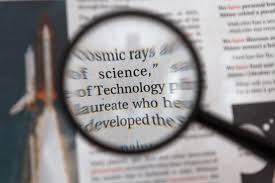
\includegraphics[width=15cm]{impresso.jpg}
\caption{Impresso, visuel \textit{© Copyright 2019 EPFL, DHLAB}}
\end{figure}
%==========Troisième technologie ==================
\item \textbf{Extrapolation - simulation des données depuis d'autres sources} 

L'une des dimensions caractéristique des \textit{\gls{bigd}}, est celle dite paradigmatique. Le nombre de données permettent elles-mêmes de déduire de nouvelles formes de sciences et de faire des découvertes\footcite{kaplan_big_2017}. Ce processus s'apparente à celui mis en place par les moines copistes ou historiens confrontés à devoir \inquote{combler les trous} de l'histoire et faire communiquer entre elles des sources différentes. Ce travail suscite depuis longtemps de nombreux débats sans qu'il existe de normes sur la manière de procéder. Time Machine soutient à priori qu'il faut veiller à précisément documenter ces techniques et les moyens déployés pour parvenir à cette \inquote{redocumentation} du passé\footcite{kaplan_big_2017}. Face aux immenses jeux de données que sont les \textit{\gls{bigd}}, les machines ont un rôle important à jouer dans la détermination du plus petit dénominateur commun capable de réunir différentes interprétations de l'histoire\footcite{kaplan_big_2017}.

Basé sur les méthodologies de l'\gls{ia}, trois moteurs de simulation, dont un moteur d'inférence permettront à Time Machine de déduire de nouvelles informations des données numérisées.

Les moteurs d'inférence ou \textit{Inference Engine} étaient un champ d'étude en \gls{ia} très populaire ; les technologies liées à l'\gls{appr} ont quelque peu réduit l'intérêt des chercheurs en la matière\footnote{Dans le cadre du stage, nous avons produit différents états de l'art sur les technologies déployées dans Time Machine, ces informations sont contenues dans la feuille de route, donnée en annexe sur la clé USB accompagnant le présent mémoire}. Time Machine entend relancer cette recherche et utiliser les données produites pour accroître son \gls{graph} de données du passé.
%==========Quatrième technologie ==================
\item \textbf{Valorisation des données afin de transformer le patrimoine en un atout pour les industries et l'économie européenne}

Afin de faciliter la découverte des données assemblées par Time Machine, une seule interface sera utilisée pour leurs valorisations, rassemblant en back-office tous les processus développés pour le projet\footnote{\cite{epfl.dhlab_dh_2019}}. 

Une première version de la future interface existe et est en cours de développement au sein du \gls{dhlab}. Cette dernière sera amenée à changer énormément au fil des avancées du projet afin de devenir un moteur de recherche diachronique : Diamond\footnote{\cite{time_machine_diamond_nodate}}.
Inclure la temporalité au sein du futur moteur de recherche implique pour Time Machine de favoriser les recherches menées sur la création de modèle 4D, actuellement dévouées à de petites échelles sans faire l'objet de standardisation\footnote{Dans le cadre du stage, nous avons produit différents états de l'art sur les technologies déployées dans Time Machine, ces informations sont contenues dans la feuille de route, figurant sur la clé USB accompagnant ce mémoire.}.
\end{enumerate}
\newpage
\begin{figure}[H]% force à placer l'image au sein de notre balise figure
\centering
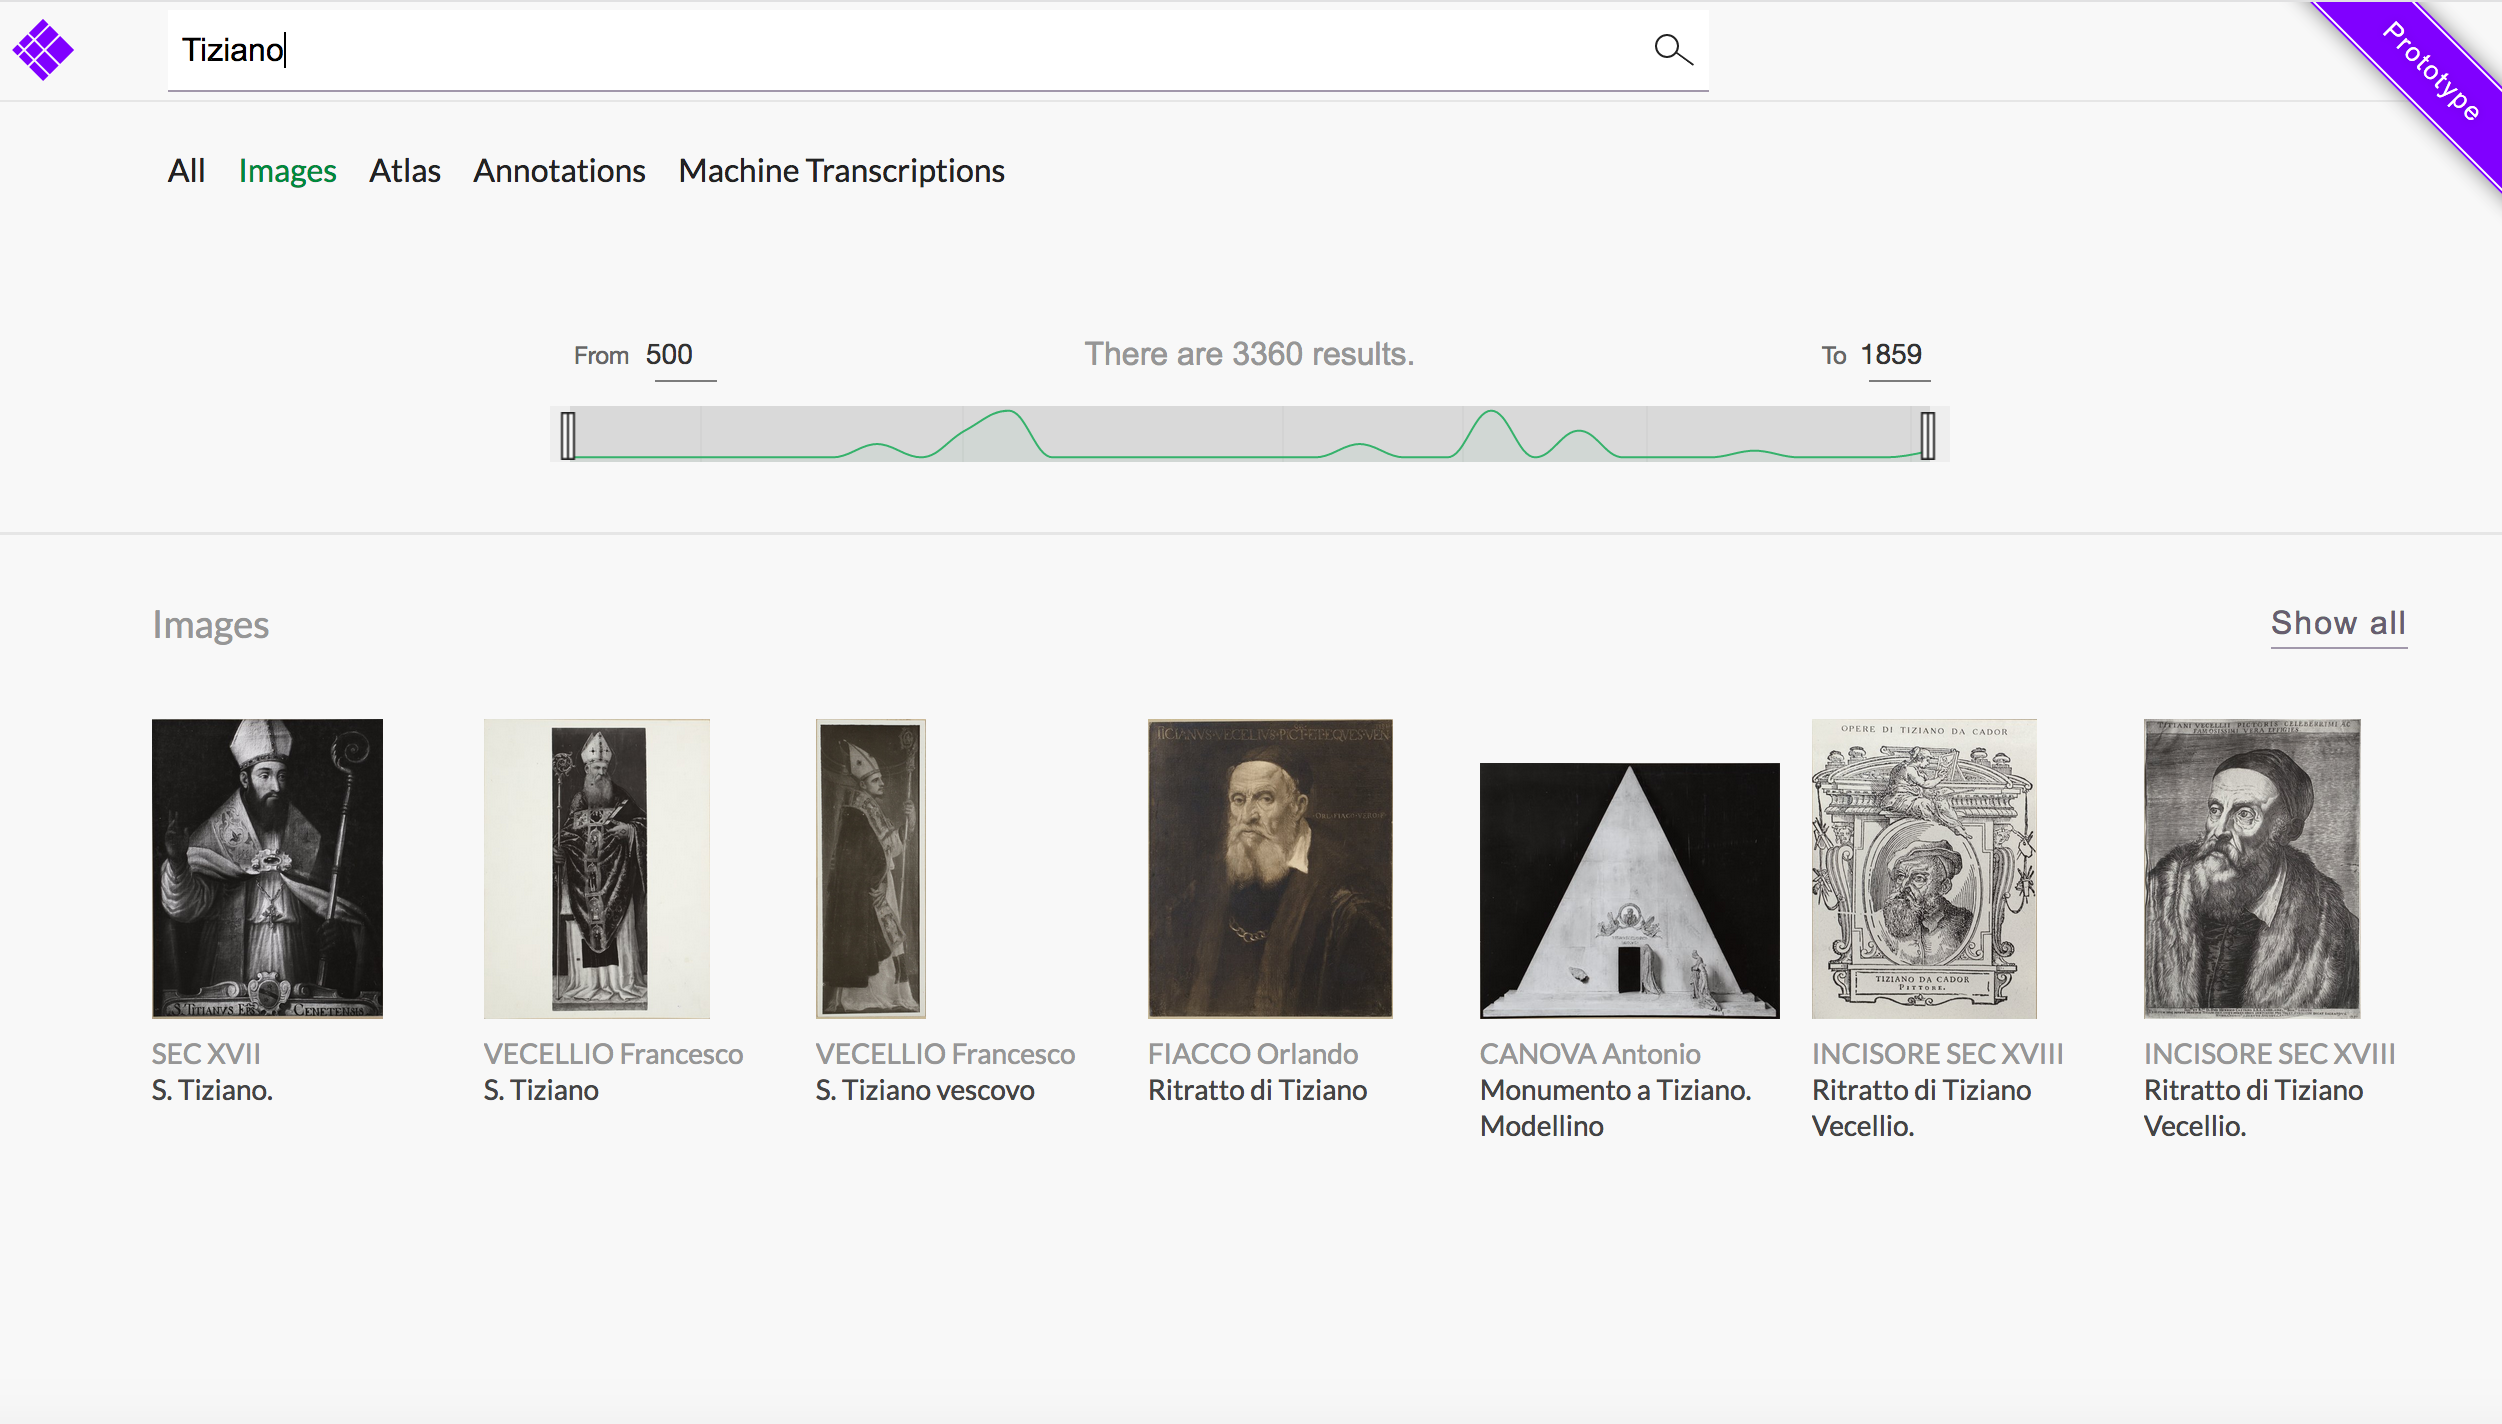
\includegraphics[width=14cm]{diamond.png}
\caption{Interface de Diamond, capture d'écran \textit{© Copyright 2019 Time Machine}}
\end{figure}

\begin{figure}[H]% force à placer l'image au sein de notre balise figure
\centering
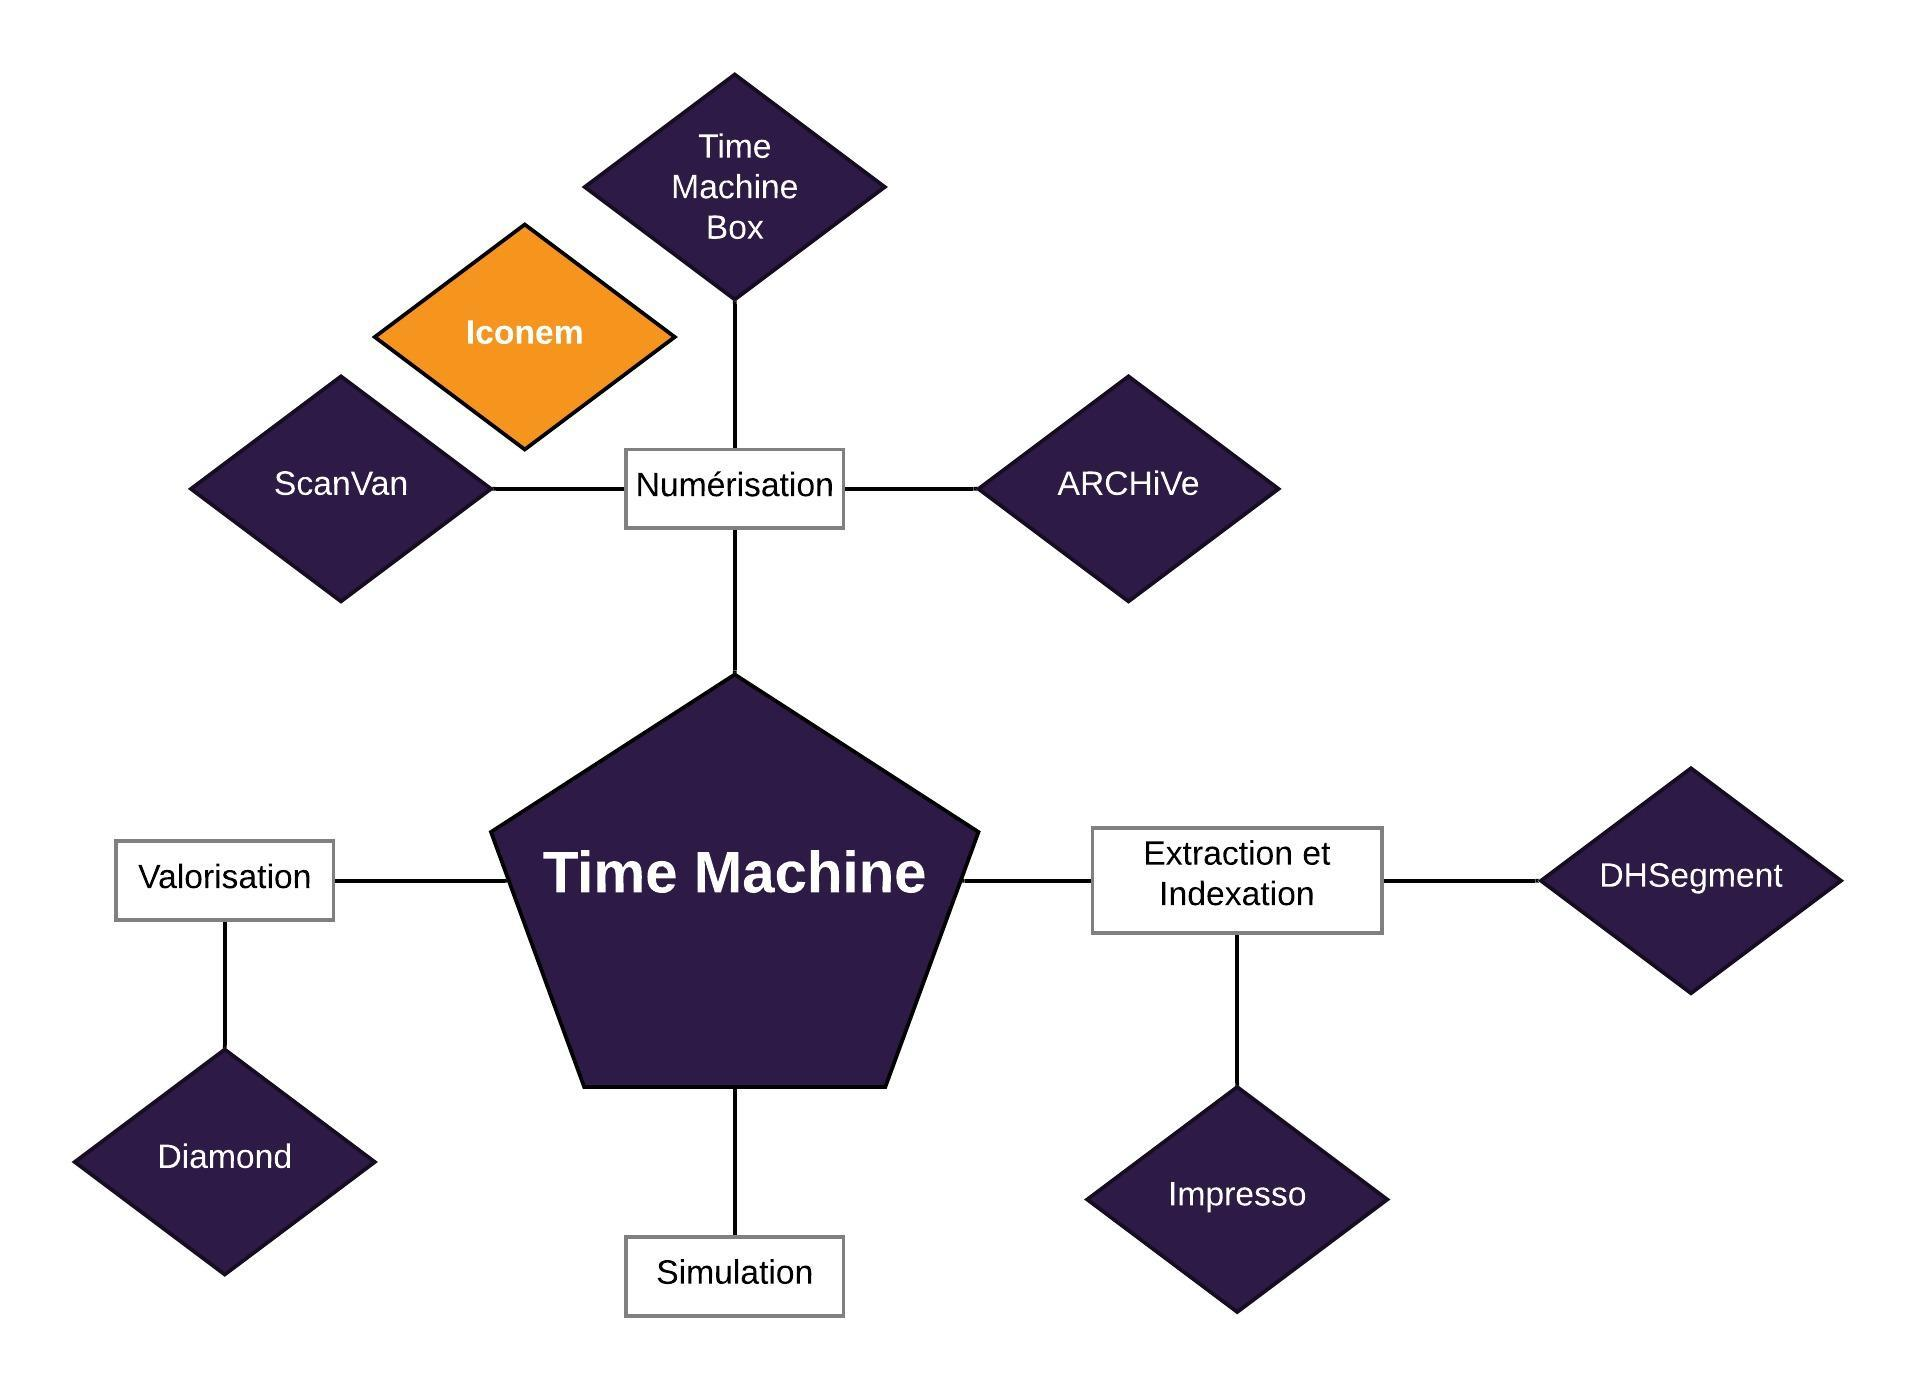
\includegraphics[scale=1.05]{technos.jpeg}
\caption{Résumé visuel des projets et technologies évoqués}
\end{figure}

\subsection{Collaboration public-privé de partenaires européens}
Des 32 partenaires initialement impliqués dans Time Machine, le consortium s'est désormais agrandi à plus de 300 institutions réparties dans 34 pays et les chiffres continuent de croître. Notre stage nous a amené à en côtoyer un grand nombre\footnote{Notamment lors de la conférence à Amsterdam, d'un séjour à Venise pour découvrir les coulisses du projet vénitien et des contacts nécessaires à la création de la feuille de route.} et offert la possibilité de questionner leurs motivations de manière informelle. De nos observations sur le terrain et de part nos activités de stagiaire, nous proposons d'établir certaines typologies, afin de mieux appréhender la multiplicité des profils et des attentes à l'encontre du projet. N'ayant pu mener de réelle étude quantitative, nous ne prétendrons pas être exhaustif : \footnote{\cite{time_machine_introduction_nodate}}. 
\begin{itemize}
\item \textbf{Les institutions culturelles et patrimoniales}

Composées de représentants des \gls{glam}, ces dernières sont à la fois intéressées par les traitements de numérisation appliqués à leurs données et par l'exploitation des résultats pour leurs propres besoins de valorisation auprès de leurs publics-cibles.
\item \textbf{Les réseaux ou consortiums}

Composés d'associations d'envergure actives dans le milieu du patrimoine, à l'instar d'Europeana\footnote{\cite{noauthor_europeana_nodate}} ou d'Icarus\footnote{\cite{icarus_icarus_nodate}}, ces dernières sont intéressées à intégrer un réseau qui leur permet à la fois de transcender leurs domaines d'activités, de rendre visibles leurs actions, d'accroître leurs membres et de participer au déploiement d'innovations technologiques applicables au sein de leurs communautés.
\item \textbf{Les laboratoires de recherche ou universités}

Composés de représentants des sciences humaines et sociales aussi bien que des sciences dures, ces centres de recherches sont motivés à l'idée de prendre une part active dans les processus d'élaboration des différents composants techniques et de traitement de ce \textit{\gls{bigd}} du passé. Ils sont également intéressés à déployer les résultats dans leurs missions d'enseignement.
\item \textbf{Les start-ups et entreprises privées}

Actives dans les domaines innovants impliqués dans Time Machine, ces dernières sont intéressées à développer de nouveaux services et modèles d'entraînement grâce aux données du \gls{graph} du passé et à valoriser ou accroître leurs compétences au sein d'un réseau de grande envergure.
\item \textbf{Les futurs exploitants}

Le \gls{graph} une fois constitué laissera la possibilité à un grand nombre d'acteurs de créer leurs propres plateformes ou services basés sur ce \textit{\gls{bigd}} du passé. Nous retrouvons ici, aux côtés des villes et des représentants des régions (le \textit{\gls{bigd}} faisant écho au mouvement des \textit{smart cities\footnote{Une ville intelligente utilise les données collectées sur internet pour mieux gérer et planifier l'utilisation de ses ressources.}}), les industries culturelles et créatives, à l'instar du fabriquant de jeu vidéo Ubisoft\footnote{\cite{ubisoft_welcome_nodate}}, les industries du tourisme, de la recherche et de l'éducation, tous intrigués par la perspective de construire de nouveaux lendemains grâce à ces données du passé.
\end{itemize}

\subsection{Un réseau de Time Machines locales}
A l'instar de Venise, d'autres villes n'ont pas attendu la fin du processus de financement pour se lancer dans la construction de leurs propres Time Machines locales. Poursuivant des objectifs divers en fonction de leurs particularités régionales et de la temporalité de leurs archives, ces initiatives sont amenées à constituer le centre du futur réseau Time Machine, qui se veut un réseau de Time Machines locales (appelées à jouer un rôle similaire à celui des \gls{agr}s),  composées de divers projets aux spécificités régionales, sous la gouvernance de la future \textit{Time Machine Organisation}. Dans un contexte au financement incertain, elles montrent également que des solutions financières locales et régionales peuvent être trouvées\footnote{\cite{rts_coup_2019}}, dont le futur réseau Time Machine\footnote{\cite{time_machine_local_nodate}}\footnote{La \textit{factsheet} du projet, donnée en annexe \ref{factsheet}, présente une liste des Times Machines locales} n'a pas encore fini d'explorer toutes les possibilités. Nous citerons ici quelques exemples parmi d'autres : 
\begin{enumerate}
\item Antwerp Time Machine (1500 - 2000)\footnote{\cite{university_of_antwerp_antwerp_nodate}}
\item Amsterdam Time Machine (1550 - 2000)\footnote{\cite{amsterdam_time_machine_amsterdam_nodate}}
\item Budapest Time Machine (1680-1990)\footnote{\cite{hungaricana_budapest_nodate}}
\item Dresden Time Machine (1200 - 2000)\footnote{\cite{noauthor_dresden_nodate}}
\item Paris Time Machine (1000 - 2000)\footnote{L'École Nationale des Chartes est membre du projet.}
\end{enumerate}

\begin{figure}[H]% force à placer l'image au sein de notre balise figure
\centering
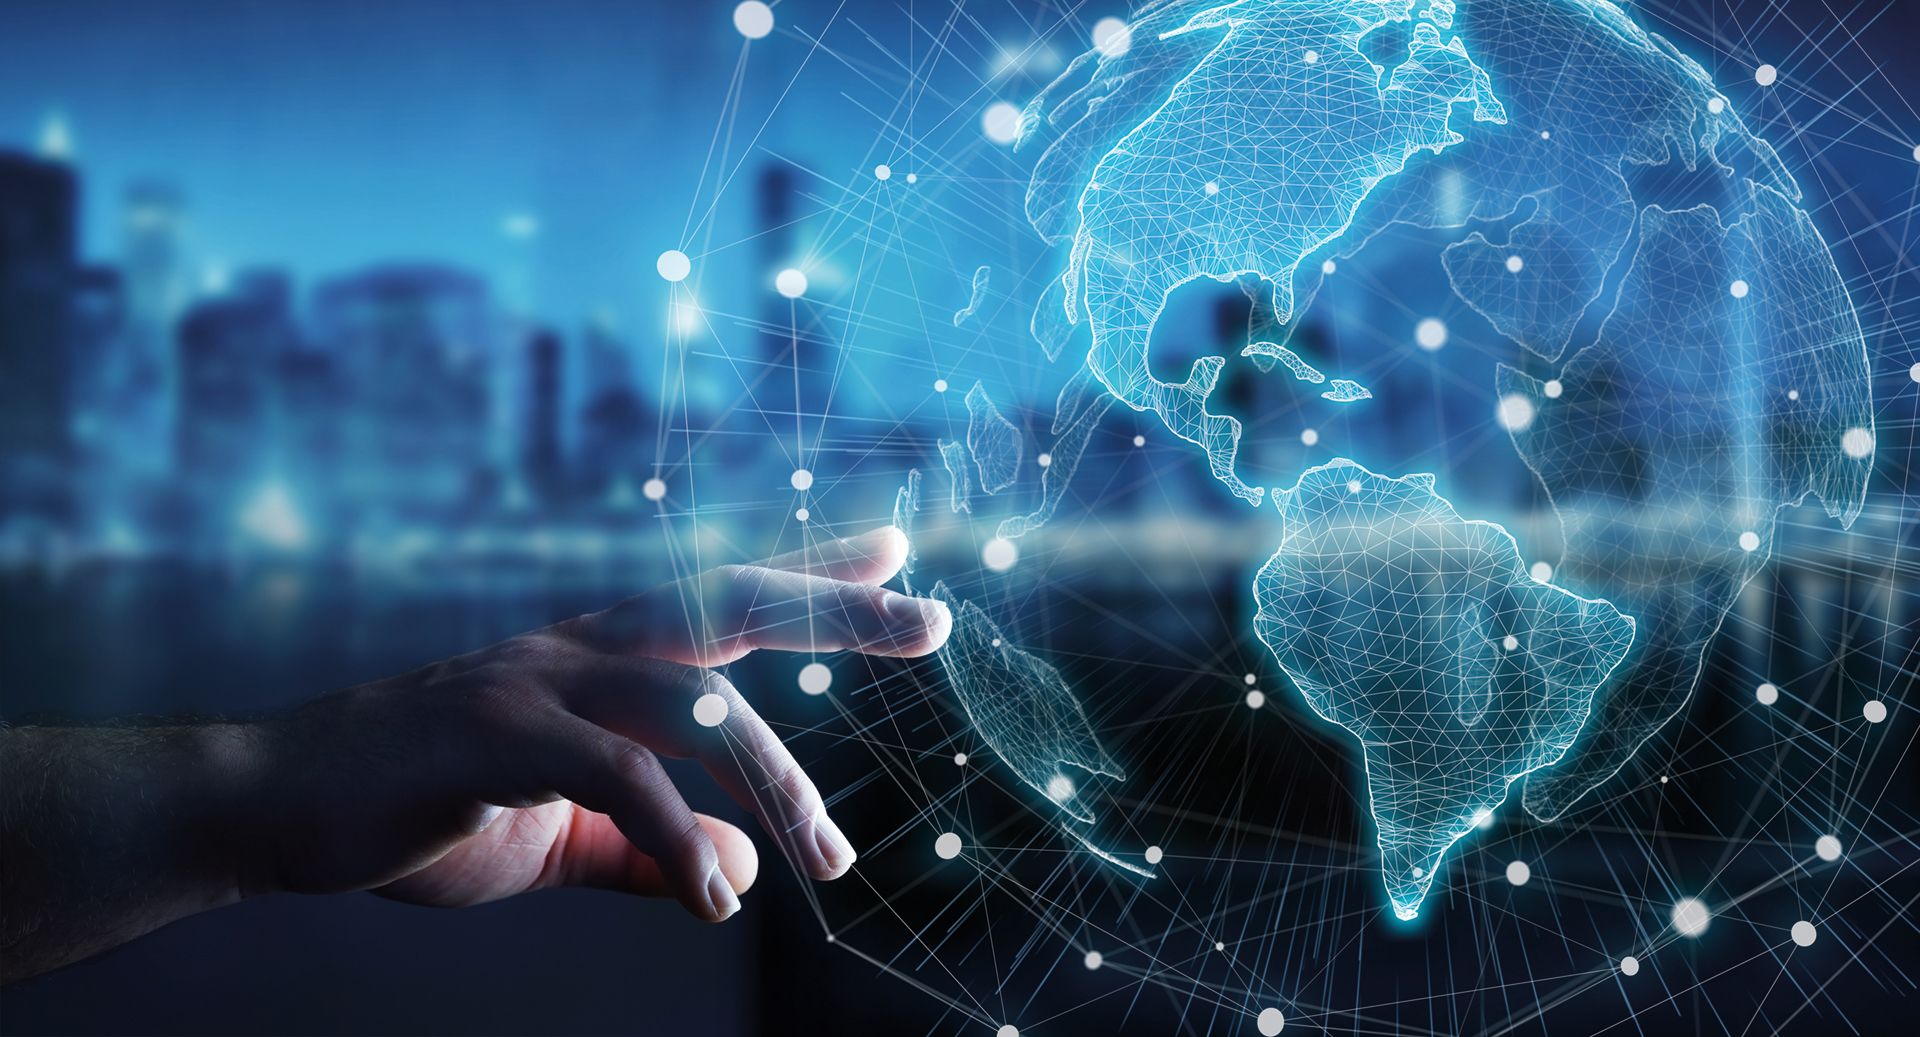
\includegraphics[width=15cm]{data_tm.jpg}
\caption{Time Machine, visualisation du réseau \textit{© Copyright 2019 Time Machine}}
\end{figure}

